% Options for packages loaded elsewhere
\PassOptionsToPackage{unicode}{hyperref}
\PassOptionsToPackage{hyphens}{url}
%
\documentclass[
]{article}
\usepackage{amsmath,amssymb}
\usepackage{iftex}
\ifPDFTeX
  \usepackage[T1]{fontenc}
  \usepackage[utf8]{inputenc}
  \usepackage{textcomp} % provide euro and other symbols
\else % if luatex or xetex
  \usepackage{unicode-math} % this also loads fontspec
  \defaultfontfeatures{Scale=MatchLowercase}
  \defaultfontfeatures[\rmfamily]{Ligatures=TeX,Scale=1}
\fi
\usepackage{lmodern}
\ifPDFTeX\else
  % xetex/luatex font selection
\fi
% Use upquote if available, for straight quotes in verbatim environments
\IfFileExists{upquote.sty}{\usepackage{upquote}}{}
\IfFileExists{microtype.sty}{% use microtype if available
  \usepackage[]{microtype}
  \UseMicrotypeSet[protrusion]{basicmath} % disable protrusion for tt fonts
}{}
\makeatletter
\@ifundefined{KOMAClassName}{% if non-KOMA class
  \IfFileExists{parskip.sty}{%
    \usepackage{parskip}
  }{% else
    \setlength{\parindent}{0pt}
    \setlength{\parskip}{6pt plus 2pt minus 1pt}}
}{% if KOMA class
  \KOMAoptions{parskip=half}}
\makeatother
\usepackage{xcolor}
\usepackage[left=1cm,right=1cm,top=2cm,bottom=2cm]{geometry}
\usepackage{color}
\usepackage{fancyvrb}
\newcommand{\VerbBar}{|}
\newcommand{\VERB}{\Verb[commandchars=\\\{\}]}
\DefineVerbatimEnvironment{Highlighting}{Verbatim}{commandchars=\\\{\}}
% Add ',fontsize=\small' for more characters per line
\usepackage{framed}
\definecolor{shadecolor}{RGB}{248,248,248}
\newenvironment{Shaded}{\begin{snugshade}}{\end{snugshade}}
\newcommand{\AlertTok}[1]{\textcolor[rgb]{0.94,0.16,0.16}{#1}}
\newcommand{\AnnotationTok}[1]{\textcolor[rgb]{0.56,0.35,0.01}{\textbf{\textit{#1}}}}
\newcommand{\AttributeTok}[1]{\textcolor[rgb]{0.13,0.29,0.53}{#1}}
\newcommand{\BaseNTok}[1]{\textcolor[rgb]{0.00,0.00,0.81}{#1}}
\newcommand{\BuiltInTok}[1]{#1}
\newcommand{\CharTok}[1]{\textcolor[rgb]{0.31,0.60,0.02}{#1}}
\newcommand{\CommentTok}[1]{\textcolor[rgb]{0.56,0.35,0.01}{\textit{#1}}}
\newcommand{\CommentVarTok}[1]{\textcolor[rgb]{0.56,0.35,0.01}{\textbf{\textit{#1}}}}
\newcommand{\ConstantTok}[1]{\textcolor[rgb]{0.56,0.35,0.01}{#1}}
\newcommand{\ControlFlowTok}[1]{\textcolor[rgb]{0.13,0.29,0.53}{\textbf{#1}}}
\newcommand{\DataTypeTok}[1]{\textcolor[rgb]{0.13,0.29,0.53}{#1}}
\newcommand{\DecValTok}[1]{\textcolor[rgb]{0.00,0.00,0.81}{#1}}
\newcommand{\DocumentationTok}[1]{\textcolor[rgb]{0.56,0.35,0.01}{\textbf{\textit{#1}}}}
\newcommand{\ErrorTok}[1]{\textcolor[rgb]{0.64,0.00,0.00}{\textbf{#1}}}
\newcommand{\ExtensionTok}[1]{#1}
\newcommand{\FloatTok}[1]{\textcolor[rgb]{0.00,0.00,0.81}{#1}}
\newcommand{\FunctionTok}[1]{\textcolor[rgb]{0.13,0.29,0.53}{\textbf{#1}}}
\newcommand{\ImportTok}[1]{#1}
\newcommand{\InformationTok}[1]{\textcolor[rgb]{0.56,0.35,0.01}{\textbf{\textit{#1}}}}
\newcommand{\KeywordTok}[1]{\textcolor[rgb]{0.13,0.29,0.53}{\textbf{#1}}}
\newcommand{\NormalTok}[1]{#1}
\newcommand{\OperatorTok}[1]{\textcolor[rgb]{0.81,0.36,0.00}{\textbf{#1}}}
\newcommand{\OtherTok}[1]{\textcolor[rgb]{0.56,0.35,0.01}{#1}}
\newcommand{\PreprocessorTok}[1]{\textcolor[rgb]{0.56,0.35,0.01}{\textit{#1}}}
\newcommand{\RegionMarkerTok}[1]{#1}
\newcommand{\SpecialCharTok}[1]{\textcolor[rgb]{0.81,0.36,0.00}{\textbf{#1}}}
\newcommand{\SpecialStringTok}[1]{\textcolor[rgb]{0.31,0.60,0.02}{#1}}
\newcommand{\StringTok}[1]{\textcolor[rgb]{0.31,0.60,0.02}{#1}}
\newcommand{\VariableTok}[1]{\textcolor[rgb]{0.00,0.00,0.00}{#1}}
\newcommand{\VerbatimStringTok}[1]{\textcolor[rgb]{0.31,0.60,0.02}{#1}}
\newcommand{\WarningTok}[1]{\textcolor[rgb]{0.56,0.35,0.01}{\textbf{\textit{#1}}}}
\usepackage{longtable,booktabs,array}
\usepackage{calc} % for calculating minipage widths
% Correct order of tables after \paragraph or \subparagraph
\usepackage{etoolbox}
\makeatletter
\patchcmd\longtable{\par}{\if@noskipsec\mbox{}\fi\par}{}{}
\makeatother
% Allow footnotes in longtable head/foot
\IfFileExists{footnotehyper.sty}{\usepackage{footnotehyper}}{\usepackage{footnote}}
\makesavenoteenv{longtable}
\usepackage{graphicx}
\makeatletter
\newsavebox\pandoc@box
\newcommand*\pandocbounded[1]{% scales image to fit in text height/width
  \sbox\pandoc@box{#1}%
  \Gscale@div\@tempa{\textheight}{\dimexpr\ht\pandoc@box+\dp\pandoc@box\relax}%
  \Gscale@div\@tempb{\linewidth}{\wd\pandoc@box}%
  \ifdim\@tempb\p@<\@tempa\p@\let\@tempa\@tempb\fi% select the smaller of both
  \ifdim\@tempa\p@<\p@\scalebox{\@tempa}{\usebox\pandoc@box}%
  \else\usebox{\pandoc@box}%
  \fi%
}
% Set default figure placement to htbp
\def\fps@figure{htbp}
\makeatother
\setlength{\emergencystretch}{3em} % prevent overfull lines
\providecommand{\tightlist}{%
  \setlength{\itemsep}{0pt}\setlength{\parskip}{0pt}}
\setcounter{secnumdepth}{-\maxdimen} % remove section numbering
\usepackage{float}
\floatplacement{figure}{H}
\renewcommand{\contentsname}{Contents}
\usepackage{mdframed}
\definecolor{shadecolor}{gray}{.90}
\renewenvironment{Shaded}{\begin{mdframed}[ backgroundcolor=shadecolor, linecolor = shadecolor, leftmargin=\dimexpr\leftmargin-2pt\relax, innerleftmargin=1.6pt, innertopmargin=5pt, skipabove=10pt,skipbelow=3pt ]}{\end{mdframed}}
\usepackage{graphicx}
\setkeys{Gin}{width=\linewidth,keepaspectratio}
\usepackage[export]{adjustbox} % útil se precisar de fallback extra
\usepackage{caption}
\captionsetup{font=small}
\usepackage{bookmark}
\IfFileExists{xurl.sty}{\usepackage{xurl}}{} % add URL line breaks if available
\urlstyle{same}
\hypersetup{
  pdftitle={Impact of COVID-19 vaccination on maternal deaths: a time series approach},
  hidelinks,
  pdfcreator={LaTeX via pandoc}}

\title{Impact of COVID-19 vaccination on maternal deaths: a time series
approach}
\author{}
\date{\vspace{-2.5em}2022}

\begin{document}
\maketitle

{
\setcounter{tocdepth}{3}
\tableofcontents
}
\newpage

\section{Abstract}

At the end of 2019, the outbreak of COVID-19 began. Later, it was
declared by the WHO as a pandemic. In Brazil, vaccination against
COVID-19 started in January 2021, only for people belonging to the
groups classified as priority, namely: health professionals,
institutionalized people aged 60 or over or with disabilities and the
village indigenous populations. During this period, there was no
relevant concern regarding the maternal population in the country on the
part of the bodies responsible for vaccine administration policies. This
population was classified as a priority group only at the beginning of
May 2021, almost 4 months after vaccination in the country was started.

It was possible to notice that, from the month of May onwards, the
number of deaths of pregnant and postpartum women began to show a
consistent downward trend, while the number of pregnant women and
postpartum women vaccinated with the first dose of the vaccine against
COVID-19 began to increase. Until that month, approximately 33 million
Brazilians had been vaccinated, a fact that could also be influencing
the downward trend in deaths of pregnant and postpartum women.

The objective of this study is to verify which factor had the greatest
impact on the fall in maternal population deaths: vaccination focused
specifically on this population or the fact that the general population
was already being vaccinated, which would confer a protective effect.
The analysis consists of a time series approach, in which daily
information on deaths and vaccination of the general population and
pregnant and postpartum women in 2021 are considered. Impulse-response
functions were used in order to verify the impact of vaccination series
on maternal deaths series. The analysis of these functions showed an
immediate impact of the first dose of the vaccine in pregnant women on
the deaths of pregnant and postpartum women.

\section{Data}

For the analysis in this document, data of pregnant and postpartum women
reported in the Influenza Epidemiological Surveillance Information
System were used, which is a national surveillance database used to
monitor respiratory infections in Brazil, known as SIVEP-Gripe. In
addition, vaccination data against COVID-19 in Brazil were also used.
The datasets were obtained on February 1, 2022, they can be found at
\url{https://opendatasus.saude.gov.br/dataset}.

The data were analyzed using the free-software R
\url{https://www.R-project.org} in version 4.1.3. Next, we present and
load the libraries used in the data analysis process.

\paragraph{Packages}\label{packages}

\begin{Shaded}
\begin{Highlighting}[]
\NormalTok{loadlibrary }\OtherTok{\textless{}{-}} \ControlFlowTok{function}\NormalTok{(x) \{}
  \ControlFlowTok{if}\NormalTok{ (}\SpecialCharTok{!}\FunctionTok{require}\NormalTok{(x, }\AttributeTok{character.only =} \ConstantTok{TRUE}\NormalTok{)) \{}
    \FunctionTok{install.packages}\NormalTok{(x, }\AttributeTok{dependencies =}\NormalTok{ T)}
    \ControlFlowTok{if}\NormalTok{ (}\SpecialCharTok{!}\FunctionTok{require}\NormalTok{(x, }\AttributeTok{character.only =} \ConstantTok{TRUE}\NormalTok{))}
      \FunctionTok{stop}\NormalTok{(}\StringTok{"Package not found"}\NormalTok{)}
\NormalTok{  \}}
\NormalTok{\}}

\NormalTok{packages }\OtherTok{\textless{}{-}}
  \FunctionTok{c}\NormalTok{(}
    \StringTok{"tseries"}\NormalTok{,}
    \StringTok{"itsmr"}\NormalTok{,}
    \StringTok{"tsibble"}\NormalTok{,}
    \StringTok{"lubridate"}\NormalTok{,}
    \StringTok{"data.table"}\NormalTok{,}
    \StringTok{"tidyr"}\NormalTok{,}
    \StringTok{"dplyr"}\NormalTok{,}
    \StringTok{"readr"}\NormalTok{,}
    \StringTok{"forecast"}\NormalTok{,}
    \StringTok{"TSA"}\NormalTok{,}
    \StringTok{"vars"}\NormalTok{,}
    \StringTok{"MTS"}\NormalTok{,}
    \StringTok{"hrbrthemes"}\NormalTok{,}
    \StringTok{"smooth"}\NormalTok{,}
    \StringTok{"RcppRoll"}\NormalTok{,}
    \StringTok{"ggplot2"}\NormalTok{,}
    \StringTok{"patchwork"}\NormalTok{,}
    \StringTok{"knitr"}
\NormalTok{  )}
\FunctionTok{lapply}\NormalTok{(packages, loadlibrary)}
\end{Highlighting}
\end{Shaded}

Our objective is to analyze data for the period of 2021, which is when
vaccination started in Brazil. We will filter the data in order to
obtain the vaccination series of the general Brazilian population and
the maternal population, as well as the series of deaths of the maternal
population. All these time series were considered between 01/03/2021 and
01/01/2022, these being the beginning and the end of the first
epidemiological week of 2021.

\paragraph{Loading the data}\label{loading-the-data}

\begin{Shaded}
\begin{Highlighting}[]
\CommentTok{\# \textgreater{} sample(1:100, 1)}
\CommentTok{\# [1] 1}
\FunctionTok{set.seed}\NormalTok{(}\DecValTok{1}\NormalTok{)}
\NormalTok{data }\OtherTok{\textless{}{-}} \FunctionTok{read\_csv}\NormalTok{(}\StringTok{\textquotesingle{}dados\_SIVEP\_Gripe\_Brasil\_01{-}02{-}22.csv\textquotesingle{}}\NormalTok{)}

\DocumentationTok{\#\# Sample period: 01/03/2021 {-} 01/01/2022}
\NormalTok{icu\_deaths }\OtherTok{\textless{}{-}}\NormalTok{ data[,}\FunctionTok{c}\NormalTok{(}\StringTok{\textquotesingle{}dt\_sint\textquotesingle{}}\NormalTok{,}\StringTok{\textquotesingle{}n\_icu\textquotesingle{}}\NormalTok{,}\StringTok{\textquotesingle{}n\_deaths\textquotesingle{}}\NormalTok{,}\StringTok{\textquotesingle{}n\_cases\textquotesingle{}}\NormalTok{)]}
\NormalTok{icu\_deaths}\SpecialCharTok{$}\NormalTok{dt\_sint }\OtherTok{\textless{}{-}} \FunctionTok{as.Date}\NormalTok{(icu\_deaths}\SpecialCharTok{$}\NormalTok{dt\_sint, }\StringTok{"\%m/\%d/\%Y"}\NormalTok{)}
\NormalTok{n }\OtherTok{\textless{}{-}} \FunctionTok{nrow}\NormalTok{(icu\_deaths)}

\DocumentationTok{\#\#\#\#\#\#\#\#\#\#\# Vaccines (total) 2021{-}2022 \#\#\#\#\#\#\#\#\#\#\#\#\#\#\#\#}
\NormalTok{vaccines }\OtherTok{\textless{}{-}} \FunctionTok{read\_csv}\NormalTok{(}\StringTok{\textquotesingle{}Vacinados\_Brasil\_01{-}02{-}22.csv\textquotesingle{}}\NormalTok{)}

\DocumentationTok{\#\#\# Sample period: 01/01/2021 {-} 01/14/2022}
\NormalTok{vaccines\_2022 }\OtherTok{\textless{}{-}}\NormalTok{ vaccines[}\DecValTok{427}\SpecialCharTok{:}\DecValTok{1661}\NormalTok{,]}
\NormalTok{vaccines\_2022}\SpecialCharTok{$}\NormalTok{vaccine\_application\_date }\OtherTok{\textless{}{-}}
  \FunctionTok{as.Date}\NormalTok{(vaccines\_2022}\SpecialCharTok{$}\NormalTok{vaccine\_application\_date, }\StringTok{"\%m/\%d/\%Y"}\NormalTok{)}
\NormalTok{vaccines\_2022 }\OtherTok{\textless{}{-}}\NormalTok{ vaccines\_2022 }\SpecialCharTok{\%\textgreater{}\%} 
  \FunctionTok{transmute}\NormalTok{(}\AttributeTok{date =}\NormalTok{ vaccine\_application\_date, }
\NormalTok{            dose\_vaccine, }
            \AttributeTok{cases =}\NormalTok{ n\_cases)}

\DocumentationTok{\#\# Filtering: vaccinated with the first dose of the vaccine}
\NormalTok{first\_dose }\OtherTok{\textless{}{-}}\NormalTok{ vaccines\_2022 }\SpecialCharTok{\%\textgreater{}\%} 
  \FunctionTok{filter}\NormalTok{(dose\_vaccine }\SpecialCharTok{==} \StringTok{\textquotesingle{}1a dose\textquotesingle{}}\NormalTok{) }\SpecialCharTok{\%\textgreater{}\%}
  \FunctionTok{group\_by}\NormalTok{(date) }\SpecialCharTok{\%\textgreater{}\%} 
  \FunctionTok{summarise}\NormalTok{(}\AttributeTok{one\_dose =} \FunctionTok{sum}\NormalTok{(cases))}

\DocumentationTok{\#\# Filtering: vaccinated with at least the second dose of the vaccine}
\NormalTok{second\_dose }\OtherTok{\textless{}{-}}\NormalTok{ vaccines\_2022 }\SpecialCharTok{\%\textgreater{}\%} 
  \FunctionTok{filter}\NormalTok{(dose\_vaccine }\SpecialCharTok{!=} \StringTok{\textquotesingle{}1a dose\textquotesingle{}}\NormalTok{) }\SpecialCharTok{\%\textgreater{}\%}
  \FunctionTok{group\_by}\NormalTok{(date) }\SpecialCharTok{\%\textgreater{}\%} 
  \FunctionTok{summarise}\NormalTok{(}\AttributeTok{immunized =} \FunctionTok{sum}\NormalTok{(cases))}

\DocumentationTok{\#\#\#\#\#\#\#\#\#\#\#\#\#\#\#\#\#\#\#\#\#\#\#\#\#\#\#\#\#\#\#\#\#\#\#\#\#\#\#\#\#\#\#\#\#\#\#\#\#\#\#\#\#\#\#}

\NormalTok{temp }\OtherTok{\textless{}{-}}\NormalTok{  icu\_deaths }\SpecialCharTok{\%\textgreater{}\%} 
  \FunctionTok{left\_join}\NormalTok{(first\_dose, }\AttributeTok{by =} \FunctionTok{c}\NormalTok{(}\StringTok{"dt\_sint"} \OtherTok{=} \StringTok{"date"}\NormalTok{)) }\SpecialCharTok{\%\textgreater{}\%}
  \FunctionTok{left\_join}\NormalTok{(second\_dose, }\AttributeTok{by =} \FunctionTok{c}\NormalTok{(}\StringTok{"dt\_sint"} \OtherTok{=} \StringTok{"date"}\NormalTok{)) }\SpecialCharTok{\%\textgreater{}\%}
  \FunctionTok{transmute}\NormalTok{(}\AttributeTok{date =}\NormalTok{ dt\_sint,}
            \AttributeTok{icu =}\NormalTok{ n\_icu,}
            \AttributeTok{deaths =}\NormalTok{ n\_deaths,}
            \AttributeTok{cases =}\NormalTok{ n\_cases,}
            \AttributeTok{first\_dose.BR =}\NormalTok{ one\_dose,}
            \AttributeTok{immunized.BR =}\NormalTok{ immunized)}

\DocumentationTok{\#\#\#\#\#\#\#\#\#\#\#\#\#\#\# Vaccines pregnant women 2022 \#\#\#\#\#\#\#\#\#\#\#\#\#\#\#\#}

\NormalTok{vaccines\_pregnant\_women }\OtherTok{\textless{}{-}}
  \FunctionTok{read\_csv}\NormalTok{(}\StringTok{\textquotesingle{}Vacinados\_GestaPuerp\_Brasil\_01{-}02{-}22.csv\textquotesingle{}}\NormalTok{)}

\NormalTok{vaccines\_pregnant\_women\_2022 }\OtherTok{\textless{}{-}}\NormalTok{ vaccines\_pregnant\_women[}\DecValTok{5}\SpecialCharTok{:}\DecValTok{790}\NormalTok{,]}
\NormalTok{vaccines\_pregnant\_women\_2022}\SpecialCharTok{$}\NormalTok{vaccine\_application\_date }\OtherTok{\textless{}{-}}
  \FunctionTok{as.Date}\NormalTok{(vaccines\_pregnant\_women\_2022}\SpecialCharTok{$}\NormalTok{vaccine\_application\_date,}
          \StringTok{"\%m/\%d/\%Y"}\NormalTok{)}

\NormalTok{vaccines\_pregnant\_women\_2022 }\OtherTok{\textless{}{-}}\NormalTok{ vaccines\_pregnant\_women\_2022 }\SpecialCharTok{\%\textgreater{}\%} 
  \FunctionTok{transmute}\NormalTok{(}\AttributeTok{date =}\NormalTok{ vaccine\_application\_date,}
\NormalTok{            dose\_vaccine,}
            \AttributeTok{cases =}\NormalTok{ n\_cases)}

\NormalTok{first\_dose\_pregnant\_women }\OtherTok{\textless{}{-}}\NormalTok{ vaccines\_pregnant\_women\_2022 }\SpecialCharTok{\%\textgreater{}\%} 
  \FunctionTok{filter}\NormalTok{(dose\_vaccine }\SpecialCharTok{==} \StringTok{\textquotesingle{}1a dose\textquotesingle{}}\NormalTok{) }\SpecialCharTok{\%\textgreater{}\%}
  \FunctionTok{group\_by}\NormalTok{(date) }\SpecialCharTok{\%\textgreater{}\%} 
  \FunctionTok{summarise}\NormalTok{(}\AttributeTok{one\_dose\_pregnant\_women =} \FunctionTok{sum}\NormalTok{(cases))}

\NormalTok{second\_dose\_pregnant\_women }\OtherTok{\textless{}{-}}\NormalTok{ vaccines\_pregnant\_women\_2022 }\SpecialCharTok{\%\textgreater{}\%} 
  \FunctionTok{filter}\NormalTok{(dose\_vaccine }\SpecialCharTok{!=} \StringTok{\textquotesingle{}1a dose\textquotesingle{}}\NormalTok{) }\SpecialCharTok{\%\textgreater{}\%}
  \FunctionTok{group\_by}\NormalTok{(date) }\SpecialCharTok{\%\textgreater{}\%} 
  \FunctionTok{summarise}\NormalTok{(}\AttributeTok{immunized\_pregnant\_women =} \FunctionTok{sum}\NormalTok{(cases))}

\NormalTok{temp\_pregnant\_women }\OtherTok{\textless{}{-}}\NormalTok{  icu\_deaths }\SpecialCharTok{\%\textgreater{}\%} 
  \FunctionTok{left\_join}\NormalTok{(first\_dose\_pregnant\_women,}
            \AttributeTok{by =} \FunctionTok{c}\NormalTok{(}\StringTok{"dt\_sint"} \OtherTok{=} \StringTok{"date"}\NormalTok{)) }\SpecialCharTok{\%\textgreater{}\%}
  \FunctionTok{left\_join}\NormalTok{(second\_dose\_pregnant\_women, }
            \AttributeTok{by =} \FunctionTok{c}\NormalTok{(}\StringTok{"dt\_sint"} \OtherTok{=} \StringTok{"date"}\NormalTok{)) }\SpecialCharTok{\%\textgreater{}\%}
  \FunctionTok{transmute}\NormalTok{(}\AttributeTok{date =}\NormalTok{ dt\_sint,}
\NormalTok{            n\_icu, }
\NormalTok{            n\_deaths,}
\NormalTok{            n\_cases, }
            \AttributeTok{first\_dose.GES =}\NormalTok{ one\_dose\_pregnant\_women, }
            \AttributeTok{immunized.GES =}\NormalTok{ immunized\_pregnant\_women) }\SpecialCharTok{\%\textgreater{}\%} 
  \FunctionTok{mutate}\NormalTok{(}\AttributeTok{first\_dose.GES =} \FunctionTok{if\_else}\NormalTok{(}\FunctionTok{is.na}\NormalTok{(first\_dose.GES),}
                                  \DecValTok{0}\NormalTok{,}
\NormalTok{                                  first\_dose.GES)) }\SpecialCharTok{\%\textgreater{}\%}
  \FunctionTok{mutate}\NormalTok{(}\AttributeTok{immunized.GES =} \FunctionTok{if\_else}\NormalTok{(}\FunctionTok{is.na}\NormalTok{(immunized.GES),}
                                 \DecValTok{0}\NormalTok{, }
\NormalTok{                                 immunized.GES))}

\CommentTok{\# Selecting variables: }

\NormalTok{data\_S }\OtherTok{\textless{}{-}}\NormalTok{ temp}
\NormalTok{data\_S}\SpecialCharTok{$}\NormalTok{first\_dose.GES }\OtherTok{\textless{}{-}}\NormalTok{ temp\_pregnant\_women}\SpecialCharTok{$}\NormalTok{first\_dose.GES}
\NormalTok{data\_S}\SpecialCharTok{$}\NormalTok{immunized.GES }\OtherTok{\textless{}{-}}\NormalTok{ temp\_pregnant\_women}\SpecialCharTok{$}\NormalTok{immunized.GES  }

\CommentTok{\# All series in the 2021 period}
\NormalTok{series }\OtherTok{\textless{}{-}}\NormalTok{ data\_S[ ,}\FunctionTok{c}\NormalTok{(}\StringTok{\textquotesingle{}date\textquotesingle{}}\NormalTok{,}
                     \StringTok{\textquotesingle{}deaths\textquotesingle{}}\NormalTok{,}
                     \StringTok{\textquotesingle{}first\_dose.BR\textquotesingle{}}\NormalTok{, }
                     \StringTok{\textquotesingle{}immunized.BR\textquotesingle{}}\NormalTok{,}
                     \StringTok{\textquotesingle{}first\_dose.GES\textquotesingle{}}\NormalTok{,}
                     \StringTok{\textquotesingle{}immunized.GES\textquotesingle{}}\NormalTok{)]}
\end{Highlighting}
\end{Shaded}

\section{Time series concepts while analyzing the data}

In order to pass on to the reader the basic concepts for understanding
the analyses, I will present and explain in a simplified way each point
that I find important for the understanding of this document as a whole,
while performing the univariate analyzes of each time series.

To begin our study, we must understand what a time series is. In a
simplified way, a time series is nothing more than a set of data
generated by a random process and observed over time. As an example of a
time series, we can think of the number of pregnant women vaccinated
daily throughout the year of 2021.

To carry out time series analysis, we need to respect some concepts on
which its theory is based. The first thing we need to check, is whether
the series in question is stationary. In practical terms, we say that a
series is stationary if it has a constant mean and variance over time.

I will show the step by step until obtaining a stationary series using
the data of this study, and in the course of the text some important new
concepts will also be addressed.

\subsection{Maternal population vaccinated with the first dose of the
COVID-19
vaccine}\label{maternal-population-vaccinated-with-the-first-dose-of-the-covid-19-vaccine}

In order to verify if the series is stationary, let's take a look at
some basic graphs.

\begin{Shaded}
\begin{Highlighting}[]
\FunctionTok{plot.ts}\NormalTok{(}\FunctionTok{ts}\NormalTok{(series}\SpecialCharTok{$}\NormalTok{first\_dose.GES), }
        \AttributeTok{xlab =} \StringTok{"Time (Days)"}\NormalTok{,}
        \AttributeTok{ylab =} \StringTok{"Number of cases (first dose)"}\NormalTok{)}
\end{Highlighting}
\end{Shaded}

\begin{center}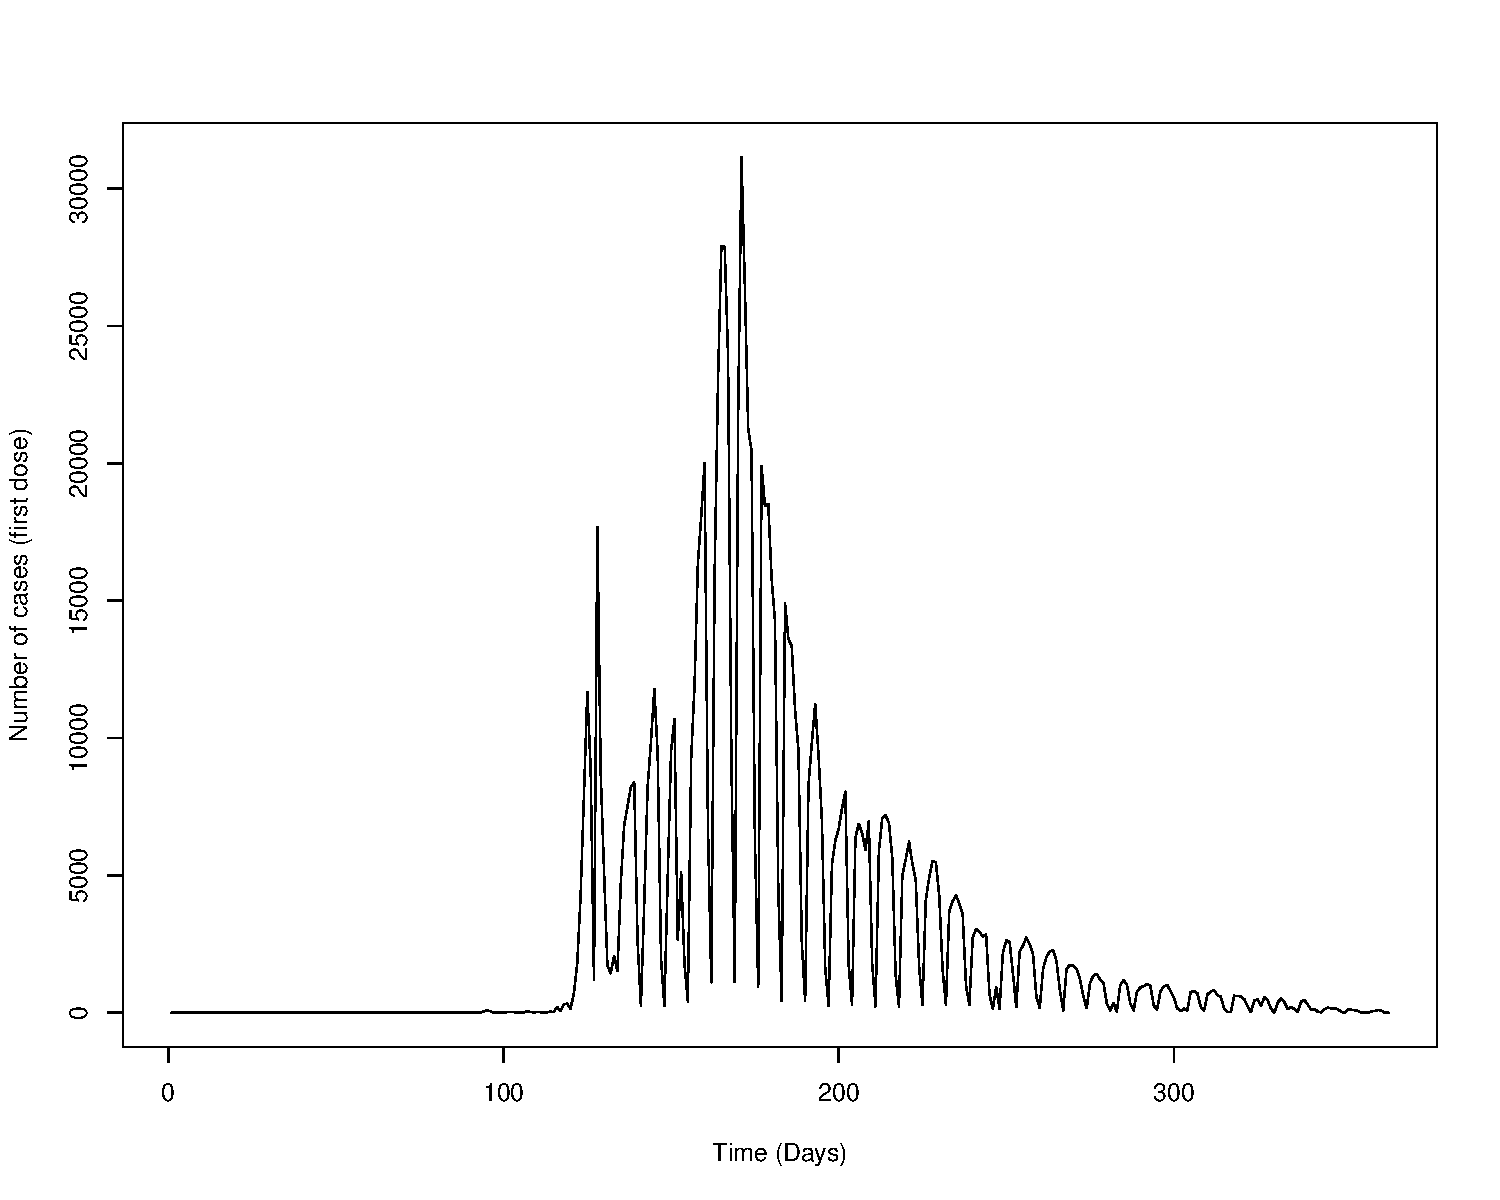
\includegraphics[width=\linewidth]{IF_results_ENG_files/figure-latex/unnamed-chunk-1-1} \end{center}

\textbf{Figure 1}: daily time series of pregnant women vaccinated with
the first dose of the vaccine in 2021.

With the time series graph, we can get a sense of its dynamics over
time. In Figure 1 for example, we can see that the number of pregnant
women being vaccinated with the first dose of the vaccine, only started
to increase around day 117 of the year 2021, before that, the number of
cases were close to zero. As a whole, this time series clearly does not
have a constant mean and variance over time.

Before we talk about autocorrelation, we should have at least a brief
understanding of the concept of lag. As stated earlier, a time series is
a set of observations over time that were generated by some random
process. A random or stochastic process, is a sequence of random
variables over time, so a time series is an observation of a random
process. Consider \(X_t\) a sequence of random variables where \(t\)
represents the time in days, as the series in question is the number of
cases of daily vaccination of pregnant women, the number of pregnant
women vaccinated on day 1 is an observation of the variable \(X_1\), the
number of pregnant women vaccinated on day 2 is an observation of the
variable \(X_2\), and so on. Given this, the lag is nothing more than
the size of the ``jump'' we make between these variables of the random
process that generated the time series. For example, when we do an
autocorrelation with a lag of 1, it means that we are looking at the
autocorrelation of \(X_1\) with \(X_2\), \(X_2\) with \(X_3\), and so
on. If the lag is equal 2, then the autocorrelation is being calculated
between \(X_1\) with \(X_3\), \(X_2\) with \(X_4\), and so on. Thus, the
autocorrelation is being calculated between the series and itself lagged
by h units of time, where in our case, h is the number of days.

The autocorrelation graph is very useful to find moving average
components when the time series is stationary. Moving average components
are values used in the modeling process that help us to eliminate
cyclical variations, consequently, as the autocorrelation graph informs
us of these components, through it we can identify possible cycles in
the time series.

\begin{Shaded}
\begin{Highlighting}[]
\FunctionTok{acf}\NormalTok{(}\FunctionTok{ts}\NormalTok{(series}\SpecialCharTok{$}\NormalTok{first\_dose.GES), }
    \AttributeTok{xlab =} \StringTok{"Lag (days)"}\NormalTok{,}
    \AttributeTok{ylab =} \StringTok{"ACF"}\NormalTok{,}
    \AttributeTok{main =} \StringTok{""}\NormalTok{,}
    \AttributeTok{lag.max =} \DecValTok{50}\NormalTok{)}
\end{Highlighting}
\end{Shaded}

\begin{center}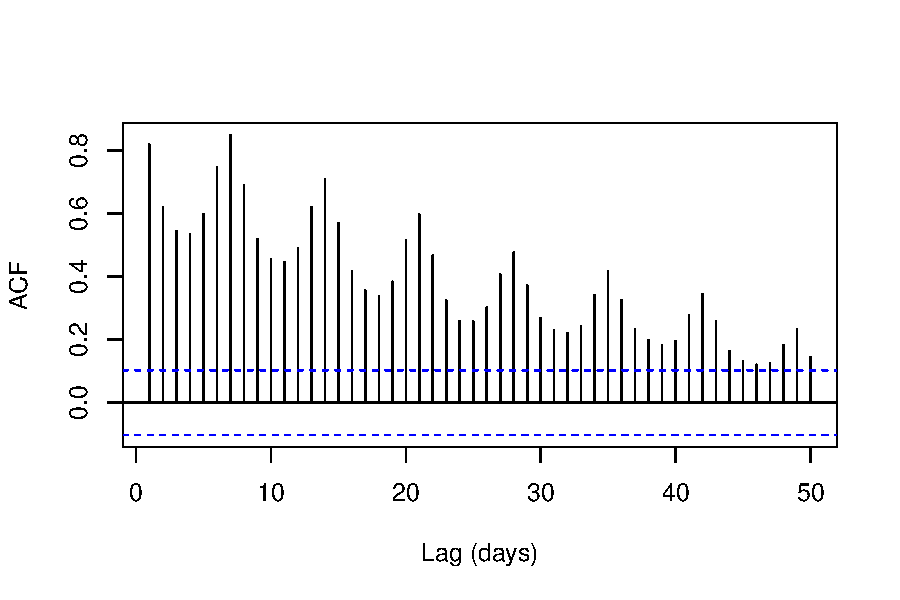
\includegraphics[width=\linewidth]{IF_results_ENG_files/figure-latex/unnamed-chunk-2-1} \end{center}

\textbf{Figure 2}: autocorrelation graph (ACF) for the time series of
pregnant women vaccinated with the first dose of the vaccine in the year
2021. The confidence bands of 95\% are presented in blue color.

In Figure 2, we can notice a natural behavior of a time series that is
not stationary, that's because when a series is stationary, most of the
graph's bars must be within the confidence bands. In addition, it is
possible to notice a repetitive behavior every 7 bars of the graph,
which suggests cycles in the series.

The partial autocorrelation graph is somehow similar to the
autocorrelation graph, but instead of being useful to find moving
average components, it is useful to find autoregressive components in a
stationary time series, which are also used in the modeling process.
Autoregressive components are related to the regression of the variable
on its own past values, similar to a linear regression model. However,
the covariate will be the lagged response variable itself. In the
modeling process, we want to use the smallest possible autoregressive
component so we can obtain the most parsimonious model. To achieve that,
we can incorporate moving averages components into the model.

\begin{Shaded}
\begin{Highlighting}[]
\FunctionTok{pacf}\NormalTok{(}\FunctionTok{ts}\NormalTok{(series}\SpecialCharTok{$}\NormalTok{first\_dose.GES), }
     \AttributeTok{xlab =} \StringTok{"Lag (days)"}\NormalTok{,}
     \AttributeTok{ylab =} \StringTok{"PACF"}\NormalTok{,}
     \AttributeTok{main =} \StringTok{""}\NormalTok{,}
     \AttributeTok{lag.max =} \DecValTok{50}\NormalTok{)}
\end{Highlighting}
\end{Shaded}

\begin{center}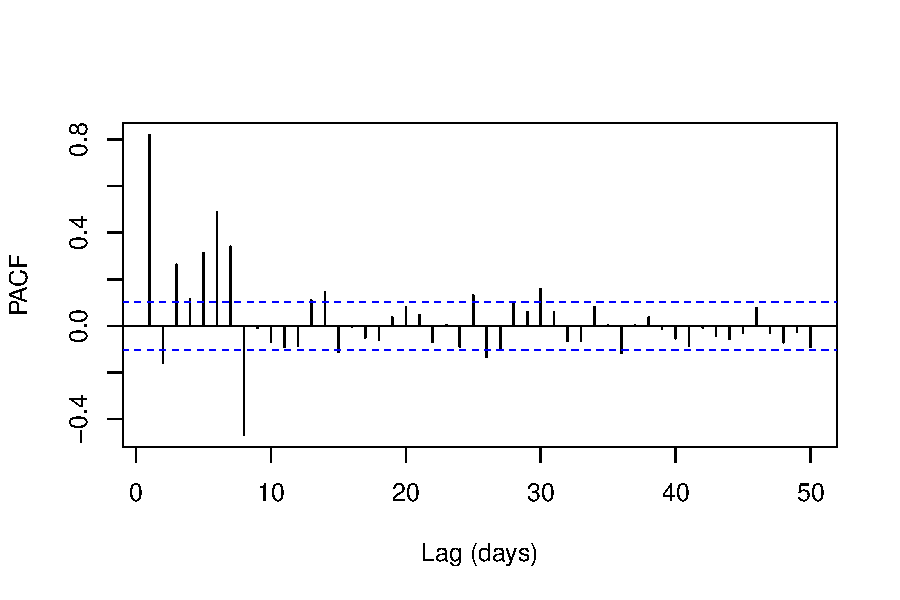
\includegraphics[width=\linewidth]{IF_results_ENG_files/figure-latex/unnamed-chunk-3-1} \end{center}

\textbf{Figure 3}: partial autocorrelation graph (PACF) for the time
series of pregnant women vaccinated with the first dose of the vaccine
in the year 2021. The confidence bands of 95\% are presented in blue
color.

The Figure 3 is a example of a partial autocorrelation graph using the
time series of pregnant women vaccinated with the first dose of the
vaccine. In practice, as for now our objective is only to achieve
stationarity, the partial autocorrelation graph will not be very
important seems it doens't tell us much if the series is not stationary.

\begin{Shaded}
\begin{Highlighting}[]
\NormalTok{TSA}\SpecialCharTok{::}\FunctionTok{periodogram}\NormalTok{(}\FunctionTok{ts}\NormalTok{(series}\SpecialCharTok{$}\NormalTok{first\_dose.GES), }
                 \AttributeTok{xlab =} \StringTok{"Frequency"}\NormalTok{,}
                 \AttributeTok{ylab =} \StringTok{"Periodogram"}\NormalTok{)}
\end{Highlighting}
\end{Shaded}

\begin{center}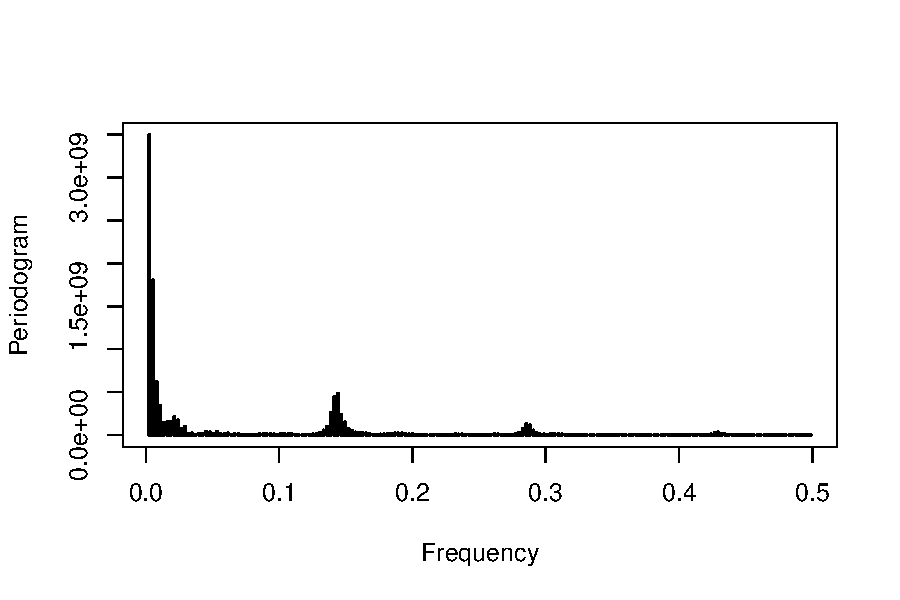
\includegraphics[width=\linewidth]{IF_results_ENG_files/figure-latex/unnamed-chunk-4-1} \end{center}

\textbf{Figure 4}: periodogram for the time series of pregnant women
vaccinated with the first dose of the vaccine.

Another useful tool to find cycles in a time series is the periodogram,
which uses frequencies to identify the possible cycles. In Figure 4, we
have a periodogram for our time series where we can notice some big
jumps, which suggests that the series has cycles in it, as we saw also
in the autocorrelation graph.

We saw before that the time series of pregnant women vaccinated with the
first dose of the vaccine has a dynamic that starts to appear in fact,
around the day 117 (115 in the data) of the year, which correspond to
04/27/2021, before that, the number of cases seems to be really close to
zero, since the vaccination actually started after 04/27/2021 by the
time series information. Because of that, for all the time series in
this study, we are going to consider the information after the moment
the vaccination started.

All the graphs we have seen so far, suggest that the series is not
stationary, to confirm this suspicion we need to apply a stationarity
test. One of the most used tests in time series to verify stationarity
in small samples is the Augmented Dickey-Fuller Test, where the null
hypothesis is that the series is not stationary.

\begin{Shaded}
\begin{Highlighting}[]
\DocumentationTok{\#\# Point where the times series dynamic starts}
\NormalTok{start\_vac }\OtherTok{\textless{}{-}} \DecValTok{115}

\DocumentationTok{\#\# Point where the time series ends}
\NormalTok{end\_vac }\OtherTok{\textless{}{-}} \DecValTok{364}

\FunctionTok{adf.test}\NormalTok{(series}\SpecialCharTok{$}\NormalTok{first\_dose.GES[start\_vac}\SpecialCharTok{:}\NormalTok{end\_vac])}
\end{Highlighting}
\end{Shaded}

\begin{verbatim}
## 
##  Augmented Dickey-Fuller Test
## 
## data:  series$first_dose.GES[start_vac:end_vac]
## Dickey-Fuller = -2.7011, Lag order = 6, p-value = 0.2806
## alternative hypothesis: stationary
\end{verbatim}

With 5\% of significance, the test points out evidences that the time
series is not stationary. Having confirmed that the series is not
stationary, we say that we have a degree of integralization, which
allows us to derive the series one time so we can try to achieve
stationarity.

\begin{Shaded}
\begin{Highlighting}[]
\DocumentationTok{\#\# 1 differentiation}
\NormalTok{firstdose\_dif1 }\OtherTok{\textless{}{-}} \FunctionTok{diff}\NormalTok{(}\FunctionTok{ts}\NormalTok{(series}\SpecialCharTok{$}\NormalTok{first\_dose.GES[start\_vac}\SpecialCharTok{:}\NormalTok{end\_vac]))}

\FunctionTok{par}\NormalTok{(}\AttributeTok{mfrow=}\FunctionTok{c}\NormalTok{(}\DecValTok{2}\NormalTok{,}\DecValTok{2}\NormalTok{))}
\FunctionTok{plot.ts}\NormalTok{(firstdose\_dif1, }
        \AttributeTok{xlab =} \StringTok{"Time"}\NormalTok{,}
        \AttributeTok{ylab =} \StringTok{"Number of cases (first dose)"}\NormalTok{)}
\NormalTok{TSA}\SpecialCharTok{::}\FunctionTok{periodogram}\NormalTok{(firstdose\_dif1, }
                 \AttributeTok{xlab =} \StringTok{"Frequency"}\NormalTok{,}
                 \AttributeTok{ylab =} \StringTok{"Periodogram"}\NormalTok{)}
\FunctionTok{acf}\NormalTok{(firstdose\_dif1, }
    \AttributeTok{xlab =} \StringTok{"Lag (days)"}\NormalTok{,}
    \AttributeTok{ylab =} \StringTok{"ACF"}\NormalTok{,}
    \AttributeTok{main =} \StringTok{""}\NormalTok{,}
    \AttributeTok{lag.max =} \DecValTok{50}\NormalTok{)}
\FunctionTok{pacf}\NormalTok{(firstdose\_dif1, }
     \AttributeTok{xlab =} \StringTok{"Lag (days)"}\NormalTok{,}
     \AttributeTok{ylab =} \StringTok{"PACF"}\NormalTok{,}
     \AttributeTok{main =} \StringTok{""}\NormalTok{,}
     \AttributeTok{lag.max =} \DecValTok{50}\NormalTok{)}
\end{Highlighting}
\end{Shaded}

\begin{center}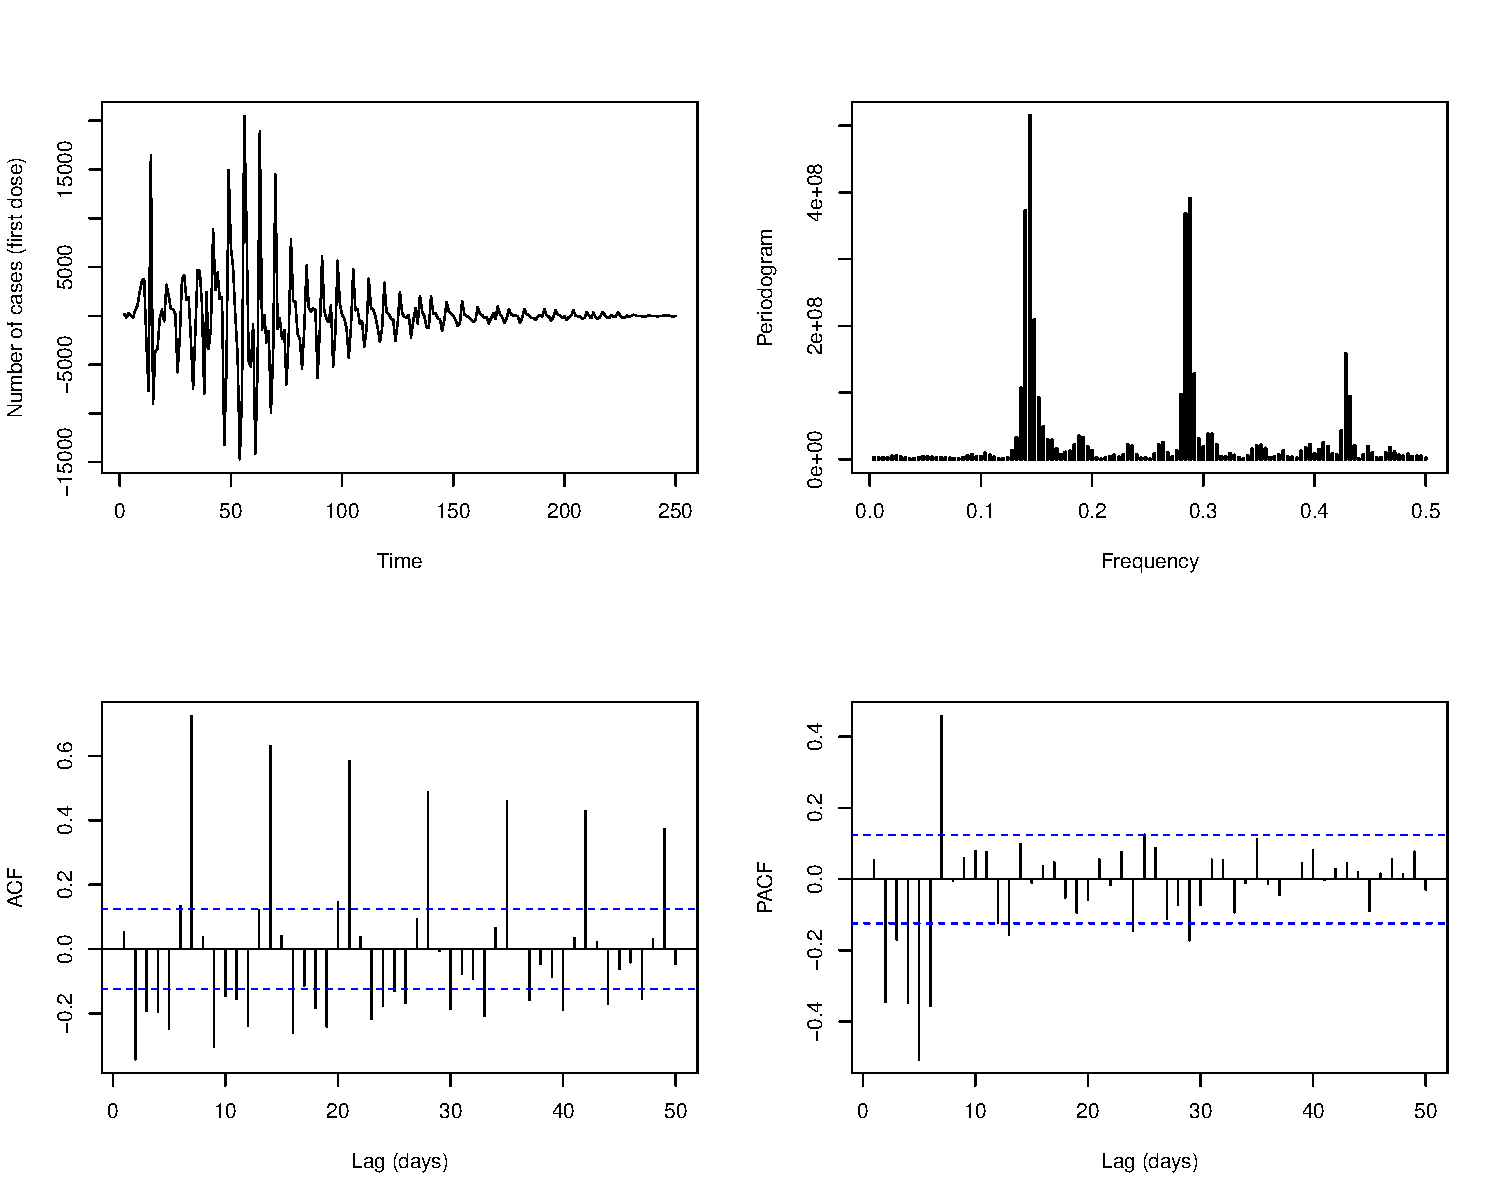
\includegraphics[width=\linewidth]{IF_results_ENG_files/figure-latex/unnamed-chunk-6-1} \end{center}

\textbf{Figure 5}: basic graphs in the analysis of time series applied
to the series of pregnant and postpartum women vaccinated with the first
dose of the COVID-19 vaccine considering one differentiation.

We can see that the jumps we saw earlier in the periodogram are now more
evident. In the autocorrelation graph, we can clearly notice a repeating
behavior that happens every 7 days, which means that we have a period of
7. Now, let's inform this period to our differentiation process and
check the time series.

\begin{Shaded}
\begin{Highlighting}[]
\DocumentationTok{\#\# Considering the 7 period information}
\NormalTok{firstdose\_dif7 }\OtherTok{\textless{}{-}} \FunctionTok{diff}\NormalTok{(firstdose\_dif1, }\DecValTok{7}\NormalTok{)}

\FunctionTok{par}\NormalTok{(}\AttributeTok{mfrow=}\FunctionTok{c}\NormalTok{(}\DecValTok{2}\NormalTok{,}\DecValTok{2}\NormalTok{))}
\FunctionTok{plot.ts}\NormalTok{(firstdose\_dif7, }
        \AttributeTok{xlab =} \StringTok{"Time"}\NormalTok{,}
        \AttributeTok{ylab =} \StringTok{"Number of cases (first dose)"}\NormalTok{)}
\NormalTok{TSA}\SpecialCharTok{::}\FunctionTok{periodogram}\NormalTok{(firstdose\_dif7, }
                 \AttributeTok{xlab =} \StringTok{"Frequency"}\NormalTok{,}
                 \AttributeTok{ylab =} \StringTok{"Periodogram"}\NormalTok{)}
\FunctionTok{acf}\NormalTok{(firstdose\_dif7, }
    \AttributeTok{xlab =} \StringTok{"Lag (days)"}\NormalTok{,}
    \AttributeTok{ylab =} \StringTok{"ACF"}\NormalTok{,}
    \AttributeTok{main =} \StringTok{""}\NormalTok{,}
    \AttributeTok{lag.max =} \DecValTok{50}\NormalTok{)}
\FunctionTok{pacf}\NormalTok{(firstdose\_dif7, }
     \AttributeTok{xlab =} \StringTok{"Lag (days)"}\NormalTok{,}
     \AttributeTok{ylab =} \StringTok{"PACF"}\NormalTok{,}
     \AttributeTok{main =} \StringTok{""}\NormalTok{,}
     \AttributeTok{lag.max =} \DecValTok{50}\NormalTok{)}
\end{Highlighting}
\end{Shaded}

\begin{center}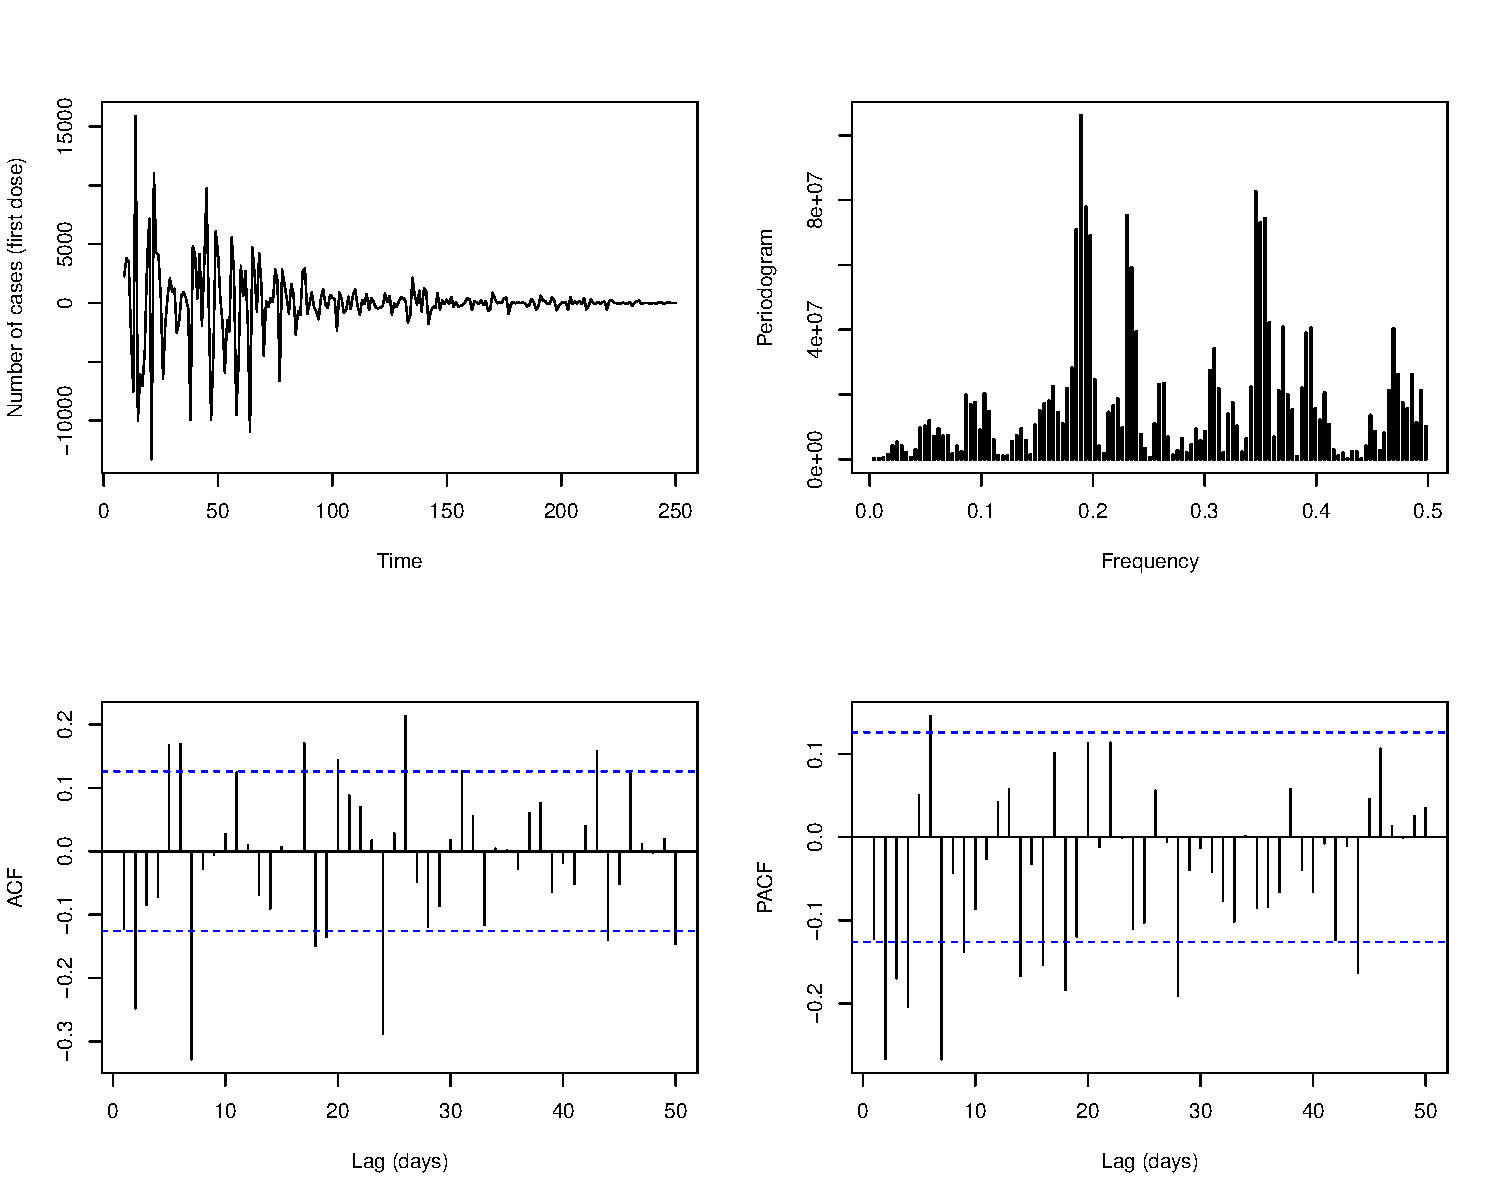
\includegraphics[width=\linewidth]{IF_results_ENG_files/figure-latex/unnamed-chunk-7-1} \end{center}

\textbf{Figure 6}: basic graphs in the analysis of time series applied
to the series of pregnant and postpartum women vaccinated with the first
dose of the COVID-19 vaccine, considering seasonal differentiation of
seven.

Now we can observe a more expected behavior of a stationary series when
we look at the periodogram and the autocorrelation graphs. However, the
variance still seems to be a little unstable, to reduce this instability
we will apply a logarithmic transformation to the data and add them to
the mean, which is a procedure widely used in the area of economics to
stabilize the variance of time series.

\begin{Shaded}
\begin{Highlighting}[]
\DocumentationTok{\#\# Summary of the time series}
\FunctionTok{summary}\NormalTok{(}\FunctionTok{ts}\NormalTok{(series}\SpecialCharTok{$}\NormalTok{first\_dose.GES[start\_vac}\SpecialCharTok{:}\NormalTok{end\_vac]))}
\end{Highlighting}
\end{Shaded}

\begin{verbatim}
##    Min. 1st Qu.  Median    Mean 3rd Qu.    Max. 
##     0.0   291.5  1352.0  4062.3  5618.8 31148.0
\end{verbatim}

\begin{Shaded}
\begin{Highlighting}[]
\DocumentationTok{\#\# \#\# Adding 4000}
\NormalTok{firstdose\_log }\OtherTok{\textless{}{-}} 
  \FunctionTok{log}\NormalTok{(}\FunctionTok{ts}\NormalTok{(series}\SpecialCharTok{$}\NormalTok{first\_dose.GES[start\_vac}\SpecialCharTok{:}\NormalTok{end\_vac]) }\SpecialCharTok{+} \DecValTok{4000}\NormalTok{)}
\NormalTok{firstdose\_dif1 }\OtherTok{\textless{}{-}} \FunctionTok{diff}\NormalTok{(firstdose\_log)}
\NormalTok{firstdose\_dif7 }\OtherTok{\textless{}{-}} \FunctionTok{diff}\NormalTok{(firstdose\_dif1, }\DecValTok{7}\NormalTok{)}

\FunctionTok{par}\NormalTok{(}\AttributeTok{mfrow=}\FunctionTok{c}\NormalTok{(}\DecValTok{2}\NormalTok{,}\DecValTok{2}\NormalTok{))}
\FunctionTok{plot.ts}\NormalTok{(firstdose\_dif7, }
        \AttributeTok{xlab =} \StringTok{"Time"}\NormalTok{,}
        \AttributeTok{ylab =} \StringTok{"Number of deaths"}\NormalTok{)}
\NormalTok{TSA}\SpecialCharTok{::}\FunctionTok{periodogram}\NormalTok{(firstdose\_dif7, }
                 \AttributeTok{xlab =} \StringTok{"Frequency"}\NormalTok{,}
                 \AttributeTok{ylab =} \StringTok{"Periodogram"}\NormalTok{)}
\FunctionTok{acf}\NormalTok{(firstdose\_dif7, }
    \AttributeTok{xlab =} \StringTok{"Lag (days)"}\NormalTok{,}
    \AttributeTok{ylab =} \StringTok{"ACF"}\NormalTok{,}
    \AttributeTok{main =} \StringTok{""}\NormalTok{,}
    \AttributeTok{lag.max =} \DecValTok{10}\NormalTok{, }
    \AttributeTok{xaxt =} \StringTok{"n"}\NormalTok{)}
\FunctionTok{axis}\NormalTok{(}\DecValTok{1}\NormalTok{, }\AttributeTok{at =} \DecValTok{1}\SpecialCharTok{:}\DecValTok{10}\NormalTok{)}
\FunctionTok{pacf}\NormalTok{(firstdose\_dif7, }
     \AttributeTok{xlab =} \StringTok{"Lag (days)"}\NormalTok{,}
     \AttributeTok{ylab =} \StringTok{"PACF"}\NormalTok{,}
     \AttributeTok{main =} \StringTok{""}\NormalTok{,}
     \AttributeTok{lag.max =} \DecValTok{10}\NormalTok{,}
     \AttributeTok{xaxt =} \StringTok{"n"}\NormalTok{)}
\FunctionTok{axis}\NormalTok{(}\DecValTok{1}\NormalTok{, }\AttributeTok{at =} \DecValTok{1}\SpecialCharTok{:}\DecValTok{10}\NormalTok{)}
\end{Highlighting}
\end{Shaded}

\begin{center}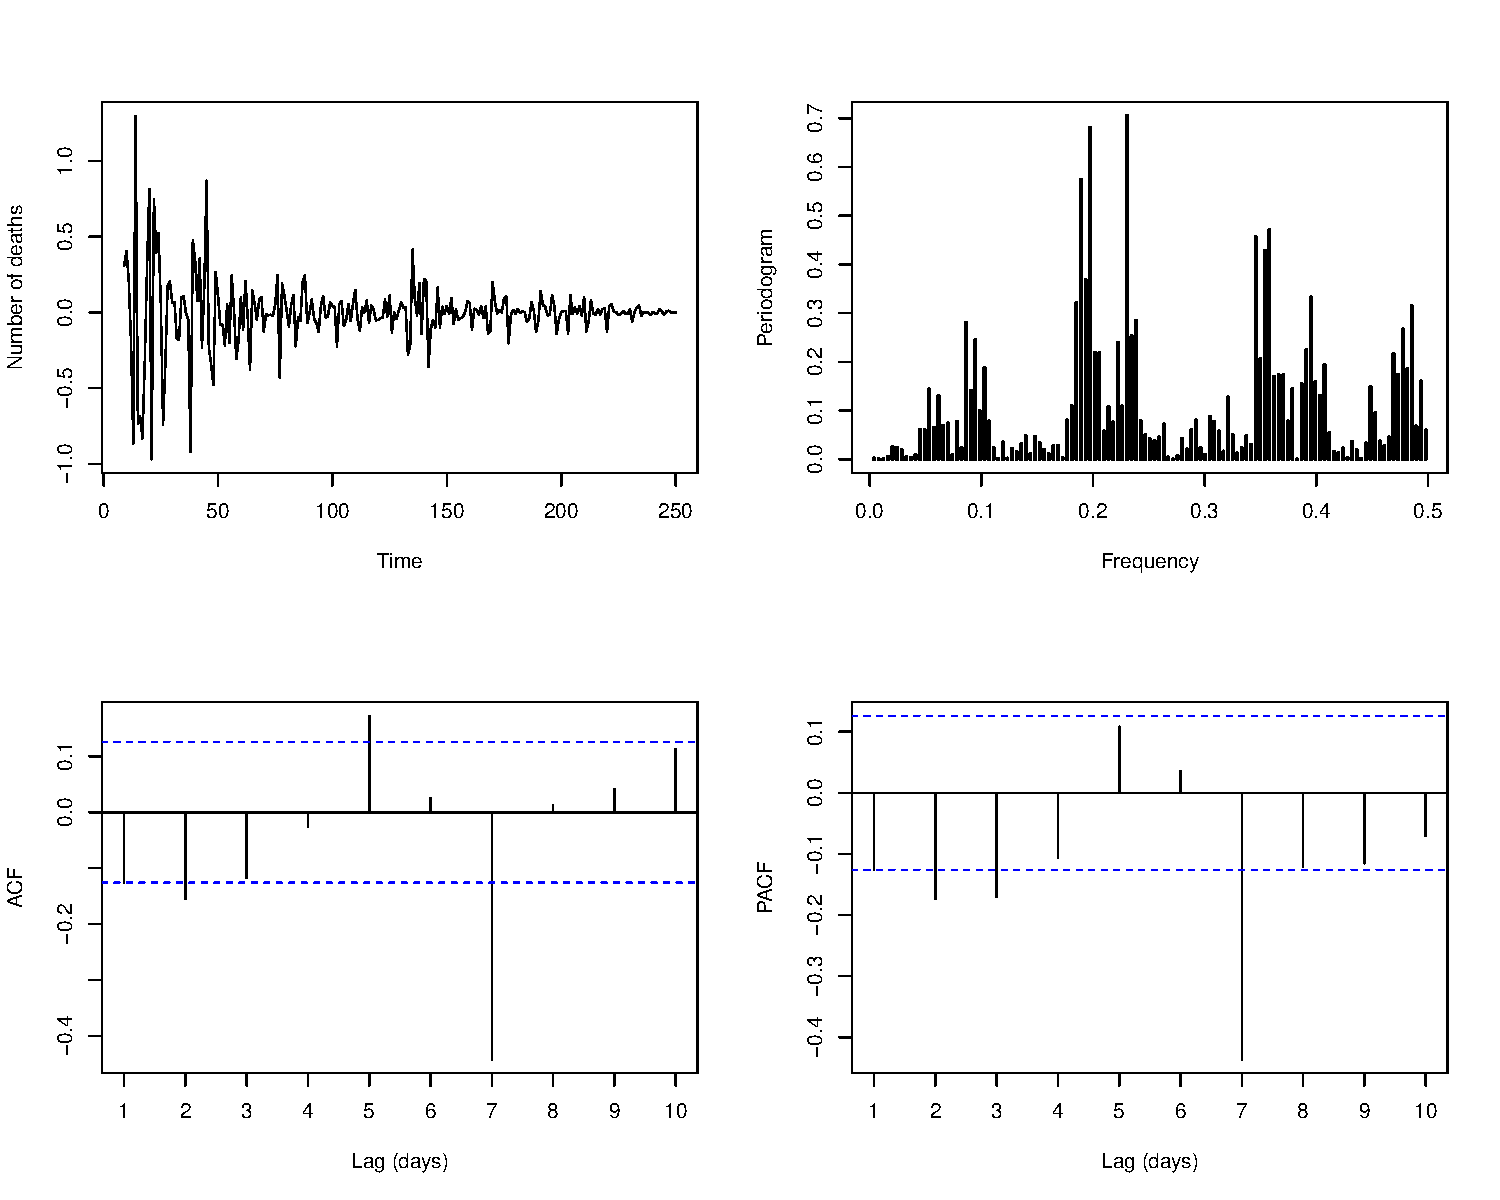
\includegraphics[width=\linewidth]{IF_results_ENG_files/figure-latex/unnamed-chunk-8-1} \end{center}

\textbf{Figure 7}: basic graphs in the analysis of time series applied
to the series of pregnant and postpartum women vaccinated with the first
dose of the COVID-19 vaccine, considering seasonal differentiation of
seven and logarithmic transformation of the data with the addition of
the mean.

Applying the Augmented Dickey-Fuller Test one more time.

\begin{Shaded}
\begin{Highlighting}[]
\FunctionTok{adf.test}\NormalTok{(firstdose\_dif7)}
\end{Highlighting}
\end{Shaded}

\begin{verbatim}
## 
##  Augmented Dickey-Fuller Test
## 
## data:  firstdose_dif7
## Dickey-Fuller = -10.505, Lag order = 6, p-value = 0.01
## alternative hypothesis: stationary
\end{verbatim}

The test points out to a stationary time series.

\subsection{Daily deaths of the maternal
population}\label{daily-deaths-of-the-maternal-population}

As we have done so far, we are going to verify if the time series of
deaths of pregnant and postpartum women is stationary. First, let's take
a look at basic time series analysis graphs.

\begin{Shaded}
\begin{Highlighting}[]
\FunctionTok{par}\NormalTok{(}\AttributeTok{mfrow=}\FunctionTok{c}\NormalTok{(}\DecValTok{2}\NormalTok{,}\DecValTok{2}\NormalTok{))}
\FunctionTok{plot.ts}\NormalTok{(}\FunctionTok{ts}\NormalTok{(series}\SpecialCharTok{$}\NormalTok{deaths[start\_vac}\SpecialCharTok{:}\NormalTok{end\_vac]),}
        \AttributeTok{xlab =} \StringTok{"Time"}\NormalTok{,}
        \AttributeTok{ylab =} \StringTok{"Number of deaths"}\NormalTok{)}
\NormalTok{TSA}\SpecialCharTok{::}\FunctionTok{periodogram}\NormalTok{(}\FunctionTok{ts}\NormalTok{(series}\SpecialCharTok{$}\NormalTok{deaths[start\_vac}\SpecialCharTok{:}\NormalTok{end\_vac]),}
                 \AttributeTok{xlab =} \StringTok{"Frequency"}\NormalTok{,}
                 \AttributeTok{ylab =} \StringTok{"Periodogram"}\NormalTok{)}
\FunctionTok{acf}\NormalTok{(}\FunctionTok{ts}\NormalTok{(series}\SpecialCharTok{$}\NormalTok{deaths[start\_vac}\SpecialCharTok{:}\NormalTok{end\_vac]),}
    \AttributeTok{xlab =} \StringTok{"Lag (days)"}\NormalTok{,}
    \AttributeTok{ylab =} \StringTok{"ACF"}\NormalTok{,}
    \AttributeTok{main =} \StringTok{""}\NormalTok{,}
    \AttributeTok{lag.max =} \DecValTok{50}\NormalTok{)}
\FunctionTok{pacf}\NormalTok{(}\FunctionTok{ts}\NormalTok{(series}\SpecialCharTok{$}\NormalTok{deaths[start\_vac}\SpecialCharTok{:}\NormalTok{end\_vac]),}
     \AttributeTok{xlab =} \StringTok{"Lag (days)"}\NormalTok{,}
     \AttributeTok{ylab =} \StringTok{"PACF"}\NormalTok{,}
     \AttributeTok{main =} \StringTok{""}\NormalTok{,}
     \AttributeTok{lag.max =} \DecValTok{50}\NormalTok{)}
\end{Highlighting}
\end{Shaded}

\begin{center}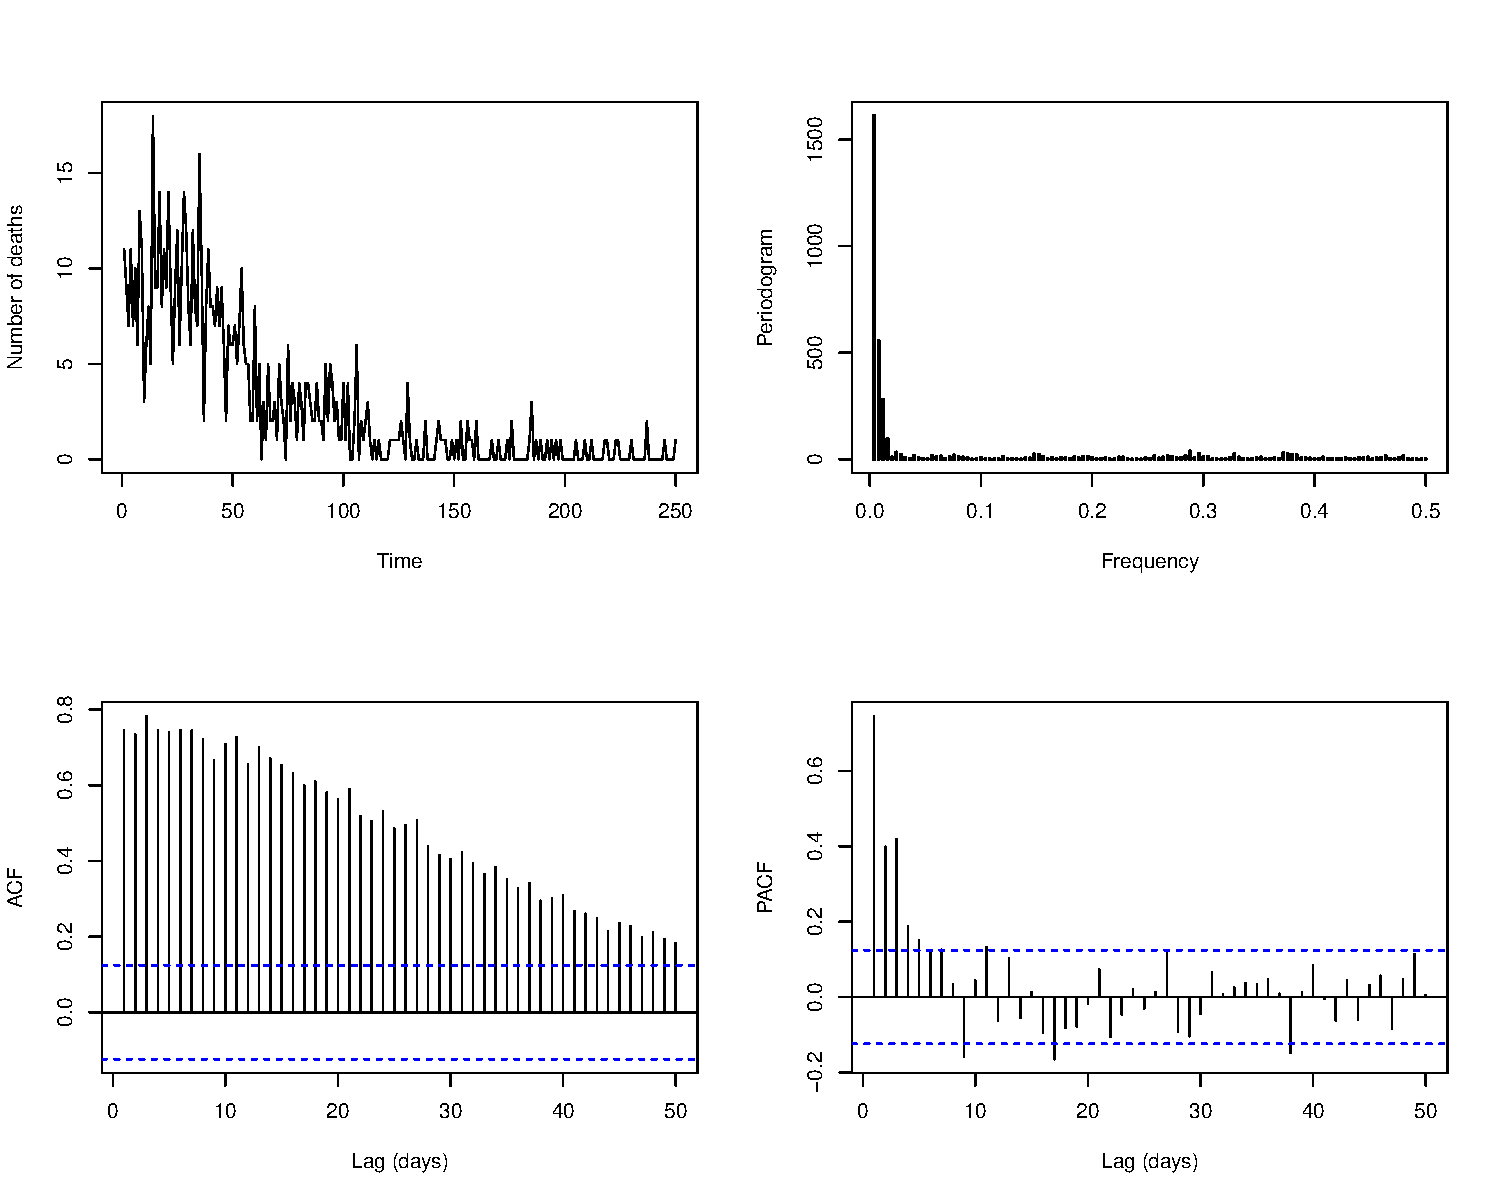
\includegraphics[width=\linewidth]{IF_results_ENG_files/figure-latex/univariate-1} \end{center}

\textbf{Figure 8}: basic graphs in the analysis of time series applied
to the series of pregnant and postpartum women deaths.

At first, the autocorrelation graphs and the periodogram do not suggest
cycles in their behavior that are evident. The time series graph
suggests that the mean and variance are not constant over time, which
goes against stationarity. To verify this assumption, we applied a
Augmented Dickey-Fuller Test.

\begin{Shaded}
\begin{Highlighting}[]
\FunctionTok{adf.test}\NormalTok{(series}\SpecialCharTok{$}\NormalTok{deaths[start\_vac}\SpecialCharTok{:}\NormalTok{end\_vac])}
\end{Highlighting}
\end{Shaded}

\begin{verbatim}
## 
##  Augmented Dickey-Fuller Test
## 
## data:  series$deaths[start_vac:end_vac]
## Dickey-Fuller = -1.4739, Lag order = 6, p-value = 0.7973
## alternative hypothesis: stationary
\end{verbatim}

The Augmented Dickey-Fuller Test showed evidence of non-stationarity. We
can apply a differentiation for better results.

\begin{Shaded}
\begin{Highlighting}[]
\NormalTok{deaths\_dif1 }\OtherTok{\textless{}{-}} \FunctionTok{diff}\NormalTok{(}\FunctionTok{ts}\NormalTok{(series}\SpecialCharTok{$}\NormalTok{deaths[start\_vac}\SpecialCharTok{:}\NormalTok{end\_vac]))}

\FunctionTok{par}\NormalTok{(}\AttributeTok{mfrow=}\FunctionTok{c}\NormalTok{(}\DecValTok{2}\NormalTok{,}\DecValTok{2}\NormalTok{))}
\FunctionTok{plot}\NormalTok{(deaths\_dif1,}
     \AttributeTok{xlab =} \StringTok{"Time"}\NormalTok{,}
     \AttributeTok{ylab =} \StringTok{"Number of deaths"}\NormalTok{)}
\NormalTok{TSA}\SpecialCharTok{::}\FunctionTok{periodogram}\NormalTok{(deaths\_dif1,}
                 \AttributeTok{xlab =} \StringTok{"Frequency"}\NormalTok{,}
                 \AttributeTok{ylab =} \StringTok{"Periodogram"}\NormalTok{)}
\FunctionTok{acf}\NormalTok{(deaths\_dif1,}
    \AttributeTok{xlab =} \StringTok{"Lag (days)"}\NormalTok{,}
    \AttributeTok{ylab =} \StringTok{"ACF"}\NormalTok{,}
    \AttributeTok{main =} \StringTok{""}\NormalTok{,}
    \AttributeTok{lag.max =} \DecValTok{50}\NormalTok{)}
\FunctionTok{pacf}\NormalTok{(deaths\_dif1,}
     \AttributeTok{xlab =} \StringTok{"Lag (days)"}\NormalTok{,}
     \AttributeTok{ylab =} \StringTok{"PACF"}\NormalTok{,}
     \AttributeTok{main =} \StringTok{""}\NormalTok{,}
     \AttributeTok{lag.max =} \DecValTok{50}\NormalTok{)}
\end{Highlighting}
\end{Shaded}

\begin{center}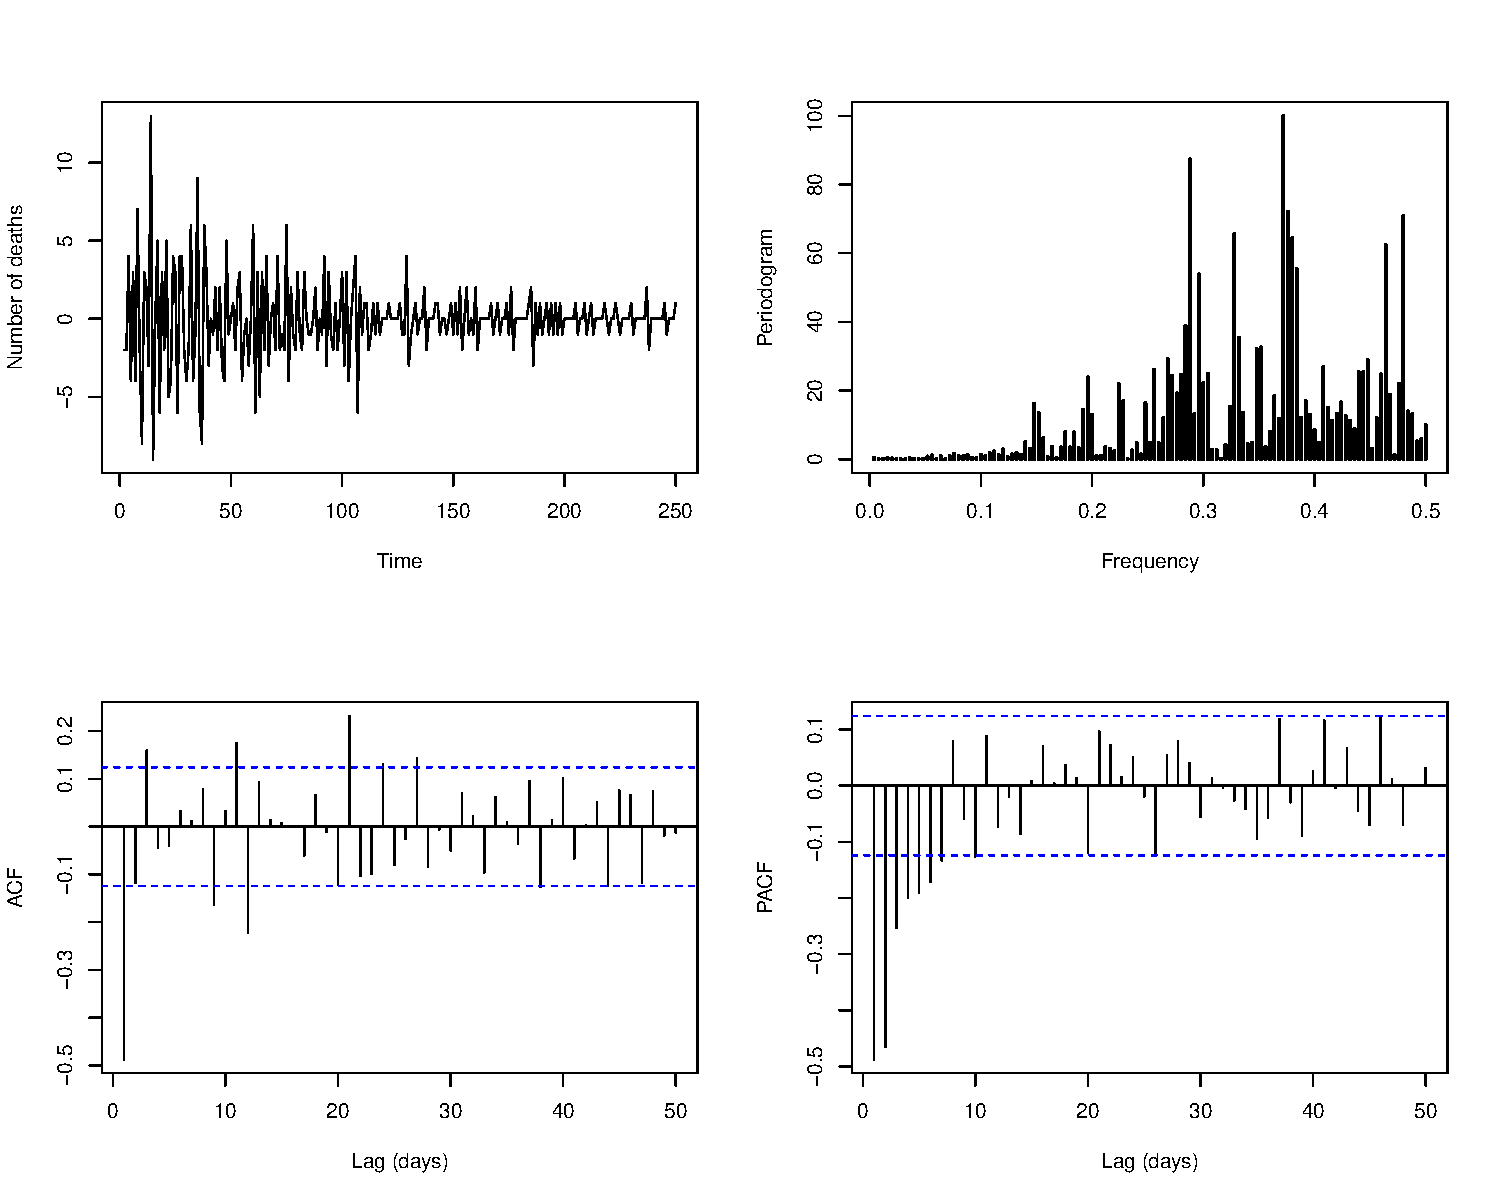
\includegraphics[width=\linewidth]{IF_results_ENG_files/figure-latex/dif1deaths-1} \end{center}

\textbf{Figure 9}: basic graphs in the analysis of time series applied
to the series of pregnant and postpartum women deaths, considering one
differentiation.

Even after a differentiation, we can observe a non-constant variance
resulting from the dynamics of the time series. To deal with this
non-constant variance, we can apply a logarithmic transformation to
stabilize it, but since we have many observations where zero deaths
occurred (95 out of 250 observations) we can change the scale by adding
the mean to the data.

\begin{Shaded}
\begin{Highlighting}[]
\DocumentationTok{\#\# Summary}
\FunctionTok{summary}\NormalTok{(}\FunctionTok{ts}\NormalTok{(series}\SpecialCharTok{$}\NormalTok{deaths[start\_vac}\SpecialCharTok{:}\NormalTok{end\_vac]))}
\end{Highlighting}
\end{Shaded}

\begin{verbatim}
##    Min. 1st Qu.  Median    Mean 3rd Qu.    Max. 
##   0.000   0.000   1.000   2.752   4.000  18.000
\end{verbatim}

\begin{Shaded}
\begin{Highlighting}[]
\DocumentationTok{\#\# Adding the mean and applying log transformation}
\NormalTok{deaths\_log }\OtherTok{\textless{}{-}} \FunctionTok{log}\NormalTok{(}\FunctionTok{ts}\NormalTok{(series}\SpecialCharTok{$}\NormalTok{deaths[start\_vac}\SpecialCharTok{:}\NormalTok{end\_vac]) }\SpecialCharTok{+} \DecValTok{3}\NormalTok{)}
\NormalTok{deaths\_dif1 }\OtherTok{\textless{}{-}} \FunctionTok{diff}\NormalTok{(deaths\_log)}

\FunctionTok{par}\NormalTok{(}\AttributeTok{mfrow=}\FunctionTok{c}\NormalTok{(}\DecValTok{2}\NormalTok{,}\DecValTok{2}\NormalTok{))}
\FunctionTok{plot.ts}\NormalTok{(deaths\_dif1,}
        \AttributeTok{xlab =} \StringTok{"Time"}\NormalTok{,}
        \AttributeTok{ylab =} \StringTok{"Number of deaths"}\NormalTok{)}
\NormalTok{TSA}\SpecialCharTok{::}\FunctionTok{periodogram}\NormalTok{(deaths\_dif1,}
                 \AttributeTok{xlab =} \StringTok{"Frequency"}\NormalTok{,}
                 \AttributeTok{ylab =} \StringTok{"Periodogram"}\NormalTok{)}
\FunctionTok{acf}\NormalTok{(deaths\_dif1,}
     \AttributeTok{xlab =} \StringTok{"Lag (days)"}\NormalTok{,}
     \AttributeTok{ylab =} \StringTok{"ACF"}\NormalTok{,}
     \AttributeTok{main =} \StringTok{""}\NormalTok{,}
     \AttributeTok{xaxt =} \StringTok{"n"}\NormalTok{,}
     \AttributeTok{lag.max =} \DecValTok{10}\NormalTok{)}
\FunctionTok{axis}\NormalTok{(}\DecValTok{1}\NormalTok{, }\AttributeTok{at =} \DecValTok{1}\SpecialCharTok{:}\DecValTok{10}\NormalTok{)}
\FunctionTok{pacf}\NormalTok{(deaths\_dif1,}
     \AttributeTok{xlab =} \StringTok{"Lag (days)"}\NormalTok{,}
     \AttributeTok{ylab =} \StringTok{"PACF"}\NormalTok{,}
     \AttributeTok{main =} \StringTok{""}\NormalTok{,}
     \AttributeTok{xaxt =} \StringTok{"n"}\NormalTok{,}
     \AttributeTok{lag.max =} \DecValTok{10}\NormalTok{)}
\FunctionTok{axis}\NormalTok{(}\DecValTok{1}\NormalTok{, }\AttributeTok{at =} \DecValTok{1}\SpecialCharTok{:}\DecValTok{10}\NormalTok{)}
\end{Highlighting}
\end{Shaded}

\begin{center}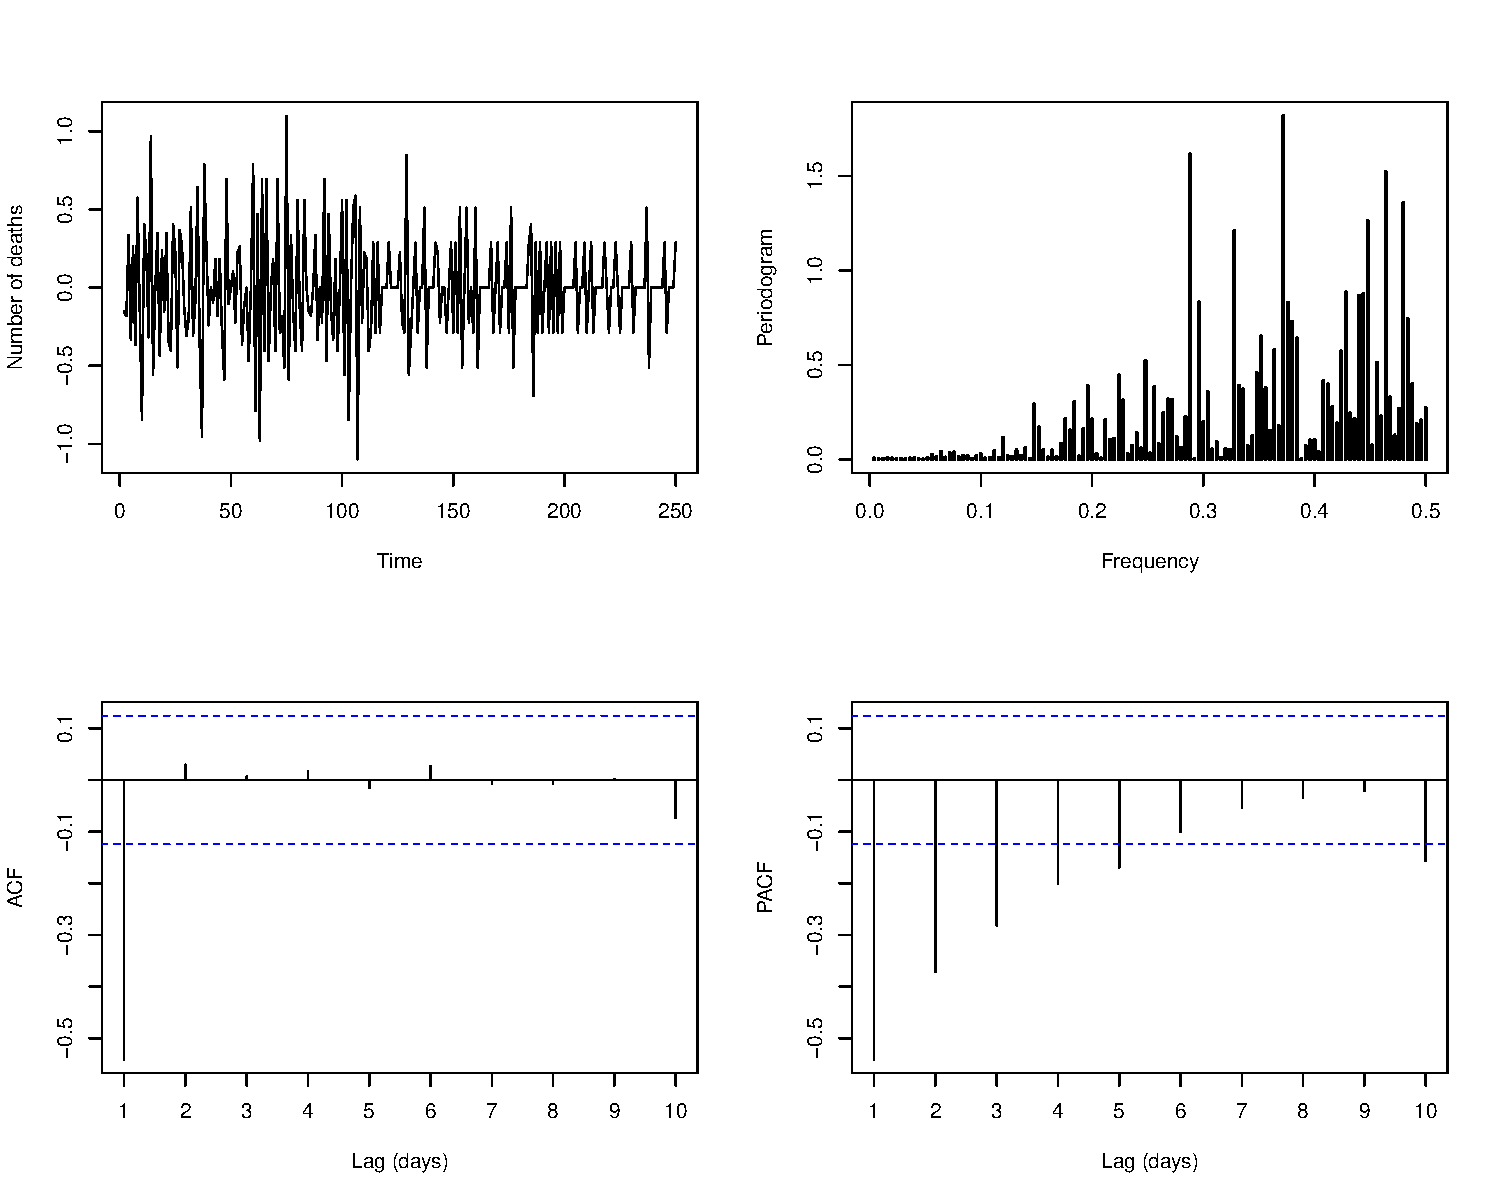
\includegraphics[width=\linewidth]{IF_results_ENG_files/figure-latex/unnamed-chunk-10-1} \end{center}

\textbf{Figure 10}: basic graphs in the analysis of time series applied
to the series of pregnant and postpartum women deaths, considering one
differentiation and logarithmic transformation of the data with the
addition of the mean.

Now we have the suspicion of stationarity. To verify it, we can apply
the Augmented Dickey-Fuller Test again.

\begin{Shaded}
\begin{Highlighting}[]
\FunctionTok{adf.test}\NormalTok{(deaths\_dif1)}
\end{Highlighting}
\end{Shaded}

\begin{verbatim}
## 
##  Augmented Dickey-Fuller Test
## 
## data:  deaths_dif1
## Dickey-Fuller = -9.3195, Lag order = 6, p-value = 0.01
## alternative hypothesis: stationary
\end{verbatim}

The test points out to the rejection of the non-stationarity hypothesis,
confirming the suspicions we had before.

\subsection{Brazilian people vaccinated with the first dose of the
COVID-19
vaccine}\label{brazilian-people-vaccinated-with-the-first-dose-of-the-covid-19-vaccine}

These data consider the general population of Brazil. we will follow the
same steps as before until we obtain stationarity.

\begin{Shaded}
\begin{Highlighting}[]
\FunctionTok{par}\NormalTok{(}\AttributeTok{mfrow=}\FunctionTok{c}\NormalTok{(}\DecValTok{2}\NormalTok{,}\DecValTok{2}\NormalTok{))}
\FunctionTok{plot.ts}\NormalTok{(}\FunctionTok{ts}\NormalTok{(series}\SpecialCharTok{$}\NormalTok{first\_dose.BR[start\_vac}\SpecialCharTok{:}\NormalTok{end\_vac]),}
        \AttributeTok{xlab =} \StringTok{"Time"}\NormalTok{,}
        \AttributeTok{ylab =} \StringTok{"Number of cases (Brazilians first dose)"}\NormalTok{)}

\NormalTok{TSA}\SpecialCharTok{::}\FunctionTok{periodogram}\NormalTok{(}\FunctionTok{ts}\NormalTok{(series}\SpecialCharTok{$}\NormalTok{first\_dose.BR[start\_vac}\SpecialCharTok{:}\NormalTok{end\_vac]),}
                 \AttributeTok{xlab =} \StringTok{"Frequency"}\NormalTok{,}
                 \AttributeTok{ylab =} \StringTok{"Periodogram"}\NormalTok{)}
\FunctionTok{acf}\NormalTok{(}\FunctionTok{ts}\NormalTok{(series}\SpecialCharTok{$}\NormalTok{first\_dose.BR[start\_vac}\SpecialCharTok{:}\NormalTok{end\_vac]),}
    \AttributeTok{xlab =} \StringTok{"Lag (days)"}\NormalTok{,}
    \AttributeTok{ylab =} \StringTok{"ACF"}\NormalTok{,}
    \AttributeTok{main =} \StringTok{""}\NormalTok{,}
    \AttributeTok{lag.max =} \DecValTok{250}\NormalTok{)}
\FunctionTok{pacf}\NormalTok{(}\FunctionTok{ts}\NormalTok{(series}\SpecialCharTok{$}\NormalTok{first\_dose.BR[start\_vac}\SpecialCharTok{:}\NormalTok{end\_vac]),}
     \AttributeTok{xlab =} \StringTok{"Lag (days)"}\NormalTok{,}
     \AttributeTok{ylab =} \StringTok{"PACF"}\NormalTok{,}
     \AttributeTok{main =} \StringTok{""}\NormalTok{,}
     \AttributeTok{lag.max =} \DecValTok{250}\NormalTok{)}
\end{Highlighting}
\end{Shaded}

\begin{center}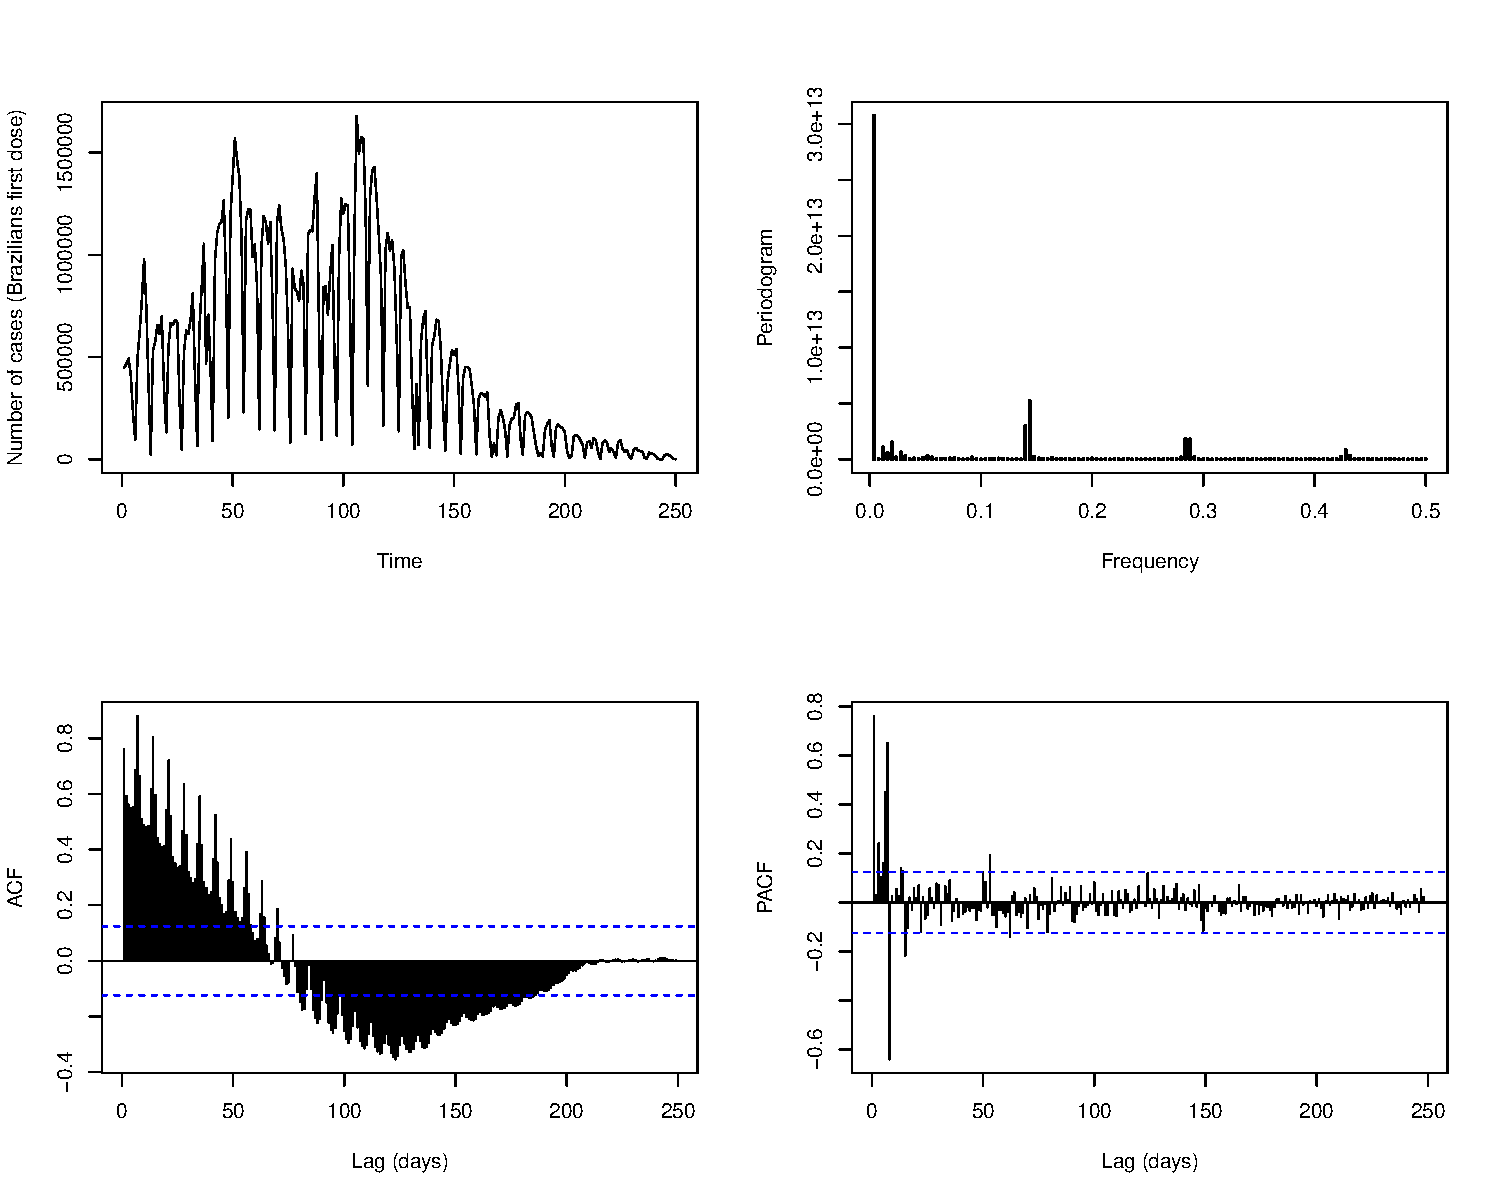
\includegraphics[width=\linewidth]{IF_results_ENG_files/figure-latex/unnamed-chunk-12-1} \end{center}

\textbf{Figure 11}: basic graphs in the analysis of time series applied
to the series of brazilian people vaccinated with the first dose of the
COVID-19 vaccine.

The time series graph suggests non-stationarity. In addition, we can see
jumps in the bars of the autocorrelation graphs and the periodogram. We
used the Augmented Dickey-Fuller Test to confirm non-stationarity.

\begin{Shaded}
\begin{Highlighting}[]
\FunctionTok{adf.test}\NormalTok{(}\FunctionTok{ts}\NormalTok{(series}\SpecialCharTok{$}\NormalTok{first\_dose.BR[start\_vac}\SpecialCharTok{:}\NormalTok{end\_vac]))}
\end{Highlighting}
\end{Shaded}

\begin{verbatim}
## 
##  Augmented Dickey-Fuller Test
## 
## data:  ts(series$first_dose.BR[start_vac:end_vac])
## Dickey-Fuller = -2.3627, Lag order = 6, p-value = 0.4231
## alternative hypothesis: stationary
\end{verbatim}

As the test shows evidence of non-stationarity, we will consider a
differentiation of 1 as a first step, and check what happens to the
series.

\begin{Shaded}
\begin{Highlighting}[]
\DocumentationTok{\#\# 1 differentiation}
\NormalTok{firstdoseBR\_dif1 }\OtherTok{\textless{}{-}}
  \FunctionTok{diff}\NormalTok{(}\FunctionTok{ts}\NormalTok{(series}\SpecialCharTok{$}\NormalTok{first\_dose.BR[start\_vac}\SpecialCharTok{:}\NormalTok{end\_vac]))}

\FunctionTok{par}\NormalTok{(}\AttributeTok{mfrow=}\FunctionTok{c}\NormalTok{(}\DecValTok{2}\NormalTok{,}\DecValTok{2}\NormalTok{))}
\FunctionTok{plot.ts}\NormalTok{(firstdoseBR\_dif1,}
        \AttributeTok{xlab =} \StringTok{"Time"}\NormalTok{,}
        \AttributeTok{ylab =} \StringTok{"Number of cases (Brazilians first dose)"}\NormalTok{)}
\NormalTok{TSA}\SpecialCharTok{::}\FunctionTok{periodogram}\NormalTok{(firstdoseBR\_dif1,}
                 \AttributeTok{xlab =} \StringTok{"Frequency"}\NormalTok{,}
                 \AttributeTok{ylab =} \StringTok{"Periodogram"}\NormalTok{)}
\FunctionTok{acf}\NormalTok{(firstdoseBR\_dif1,}
    \AttributeTok{xlab =} \StringTok{"Lag (days)"}\NormalTok{,}
    \AttributeTok{ylab =} \StringTok{"ACF"}\NormalTok{,}
    \AttributeTok{main =} \StringTok{""}\NormalTok{,}
    \AttributeTok{lag.max =} \DecValTok{50}\NormalTok{)}
\FunctionTok{pacf}\NormalTok{(firstdoseBR\_dif1,}
     \AttributeTok{xlab =} \StringTok{"Lag (days)"}\NormalTok{,}
     \AttributeTok{ylab =} \StringTok{"PACF"}\NormalTok{,}
     \AttributeTok{main =} \StringTok{""}\NormalTok{,}
     \AttributeTok{lag.max =} \DecValTok{50}\NormalTok{)}
\end{Highlighting}
\end{Shaded}

\begin{center}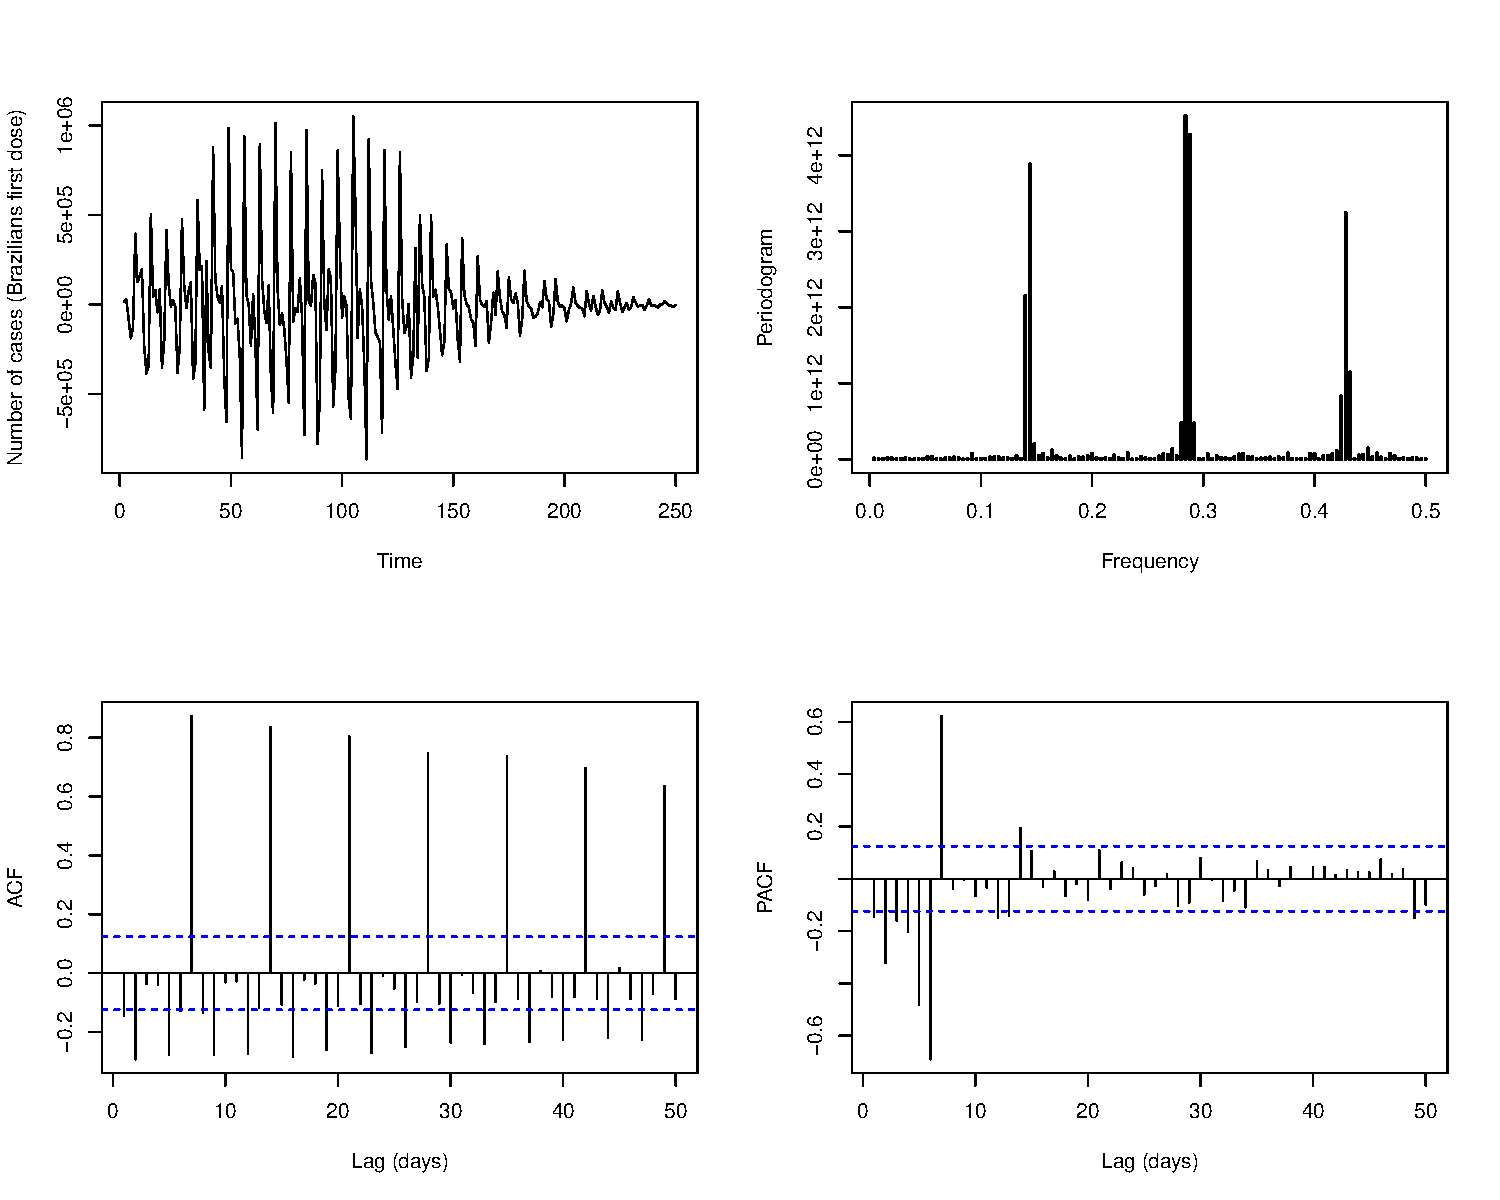
\includegraphics[width=\linewidth]{IF_results_ENG_files/figure-latex/unnamed-chunk-14-1} \end{center}

\textbf{Figure 12}: basic graphs in the analysis of time series applied
to the series of brazilian people vaccinated with the first dose of the
COVID-19 vaccine, considering one differentiation.

The jumps between graph bars are now more evident. Also, it is possible
to identify a period of 7. Now, we need to include this information in
the differentiation.

\begin{Shaded}
\begin{Highlighting}[]
\DocumentationTok{\#\# Considering the 7 period information}
\NormalTok{firstdoseBR\_dif7 }\OtherTok{\textless{}{-}} \FunctionTok{diff}\NormalTok{(firstdoseBR\_dif1, }\DecValTok{7}\NormalTok{)}

\FunctionTok{par}\NormalTok{(}\AttributeTok{mfrow=}\FunctionTok{c}\NormalTok{(}\DecValTok{2}\NormalTok{,}\DecValTok{2}\NormalTok{))}
\FunctionTok{plot.ts}\NormalTok{(firstdoseBR\_dif7,}
        \AttributeTok{xlab =} \StringTok{"Time"}\NormalTok{,}
        \AttributeTok{ylab =} \StringTok{"Number of cases (Brazilians first dose)"}\NormalTok{)}
\NormalTok{TSA}\SpecialCharTok{::}\FunctionTok{periodogram}\NormalTok{(firstdoseBR\_dif7,}
                 \AttributeTok{xlab =} \StringTok{"Frequency"}\NormalTok{,}
                 \AttributeTok{ylab =} \StringTok{"Periodogram"}\NormalTok{)}
\FunctionTok{acf}\NormalTok{(firstdoseBR\_dif7,}
    \AttributeTok{xlab =} \StringTok{"Lag (days)"}\NormalTok{,}
    \AttributeTok{ylab =} \StringTok{"ACF"}\NormalTok{,}
    \AttributeTok{main =} \StringTok{""}\NormalTok{,}
    \AttributeTok{lag.max =} \DecValTok{50}\NormalTok{)}
\FunctionTok{pacf}\NormalTok{(firstdoseBR\_dif7,}
     \AttributeTok{xlab =} \StringTok{"Lag (days)"}\NormalTok{,}
     \AttributeTok{ylab =} \StringTok{"PACF"}\NormalTok{,}
     \AttributeTok{main =} \StringTok{""}\NormalTok{,}
     \AttributeTok{lag.max =} \DecValTok{50}\NormalTok{)}
\end{Highlighting}
\end{Shaded}

\begin{center}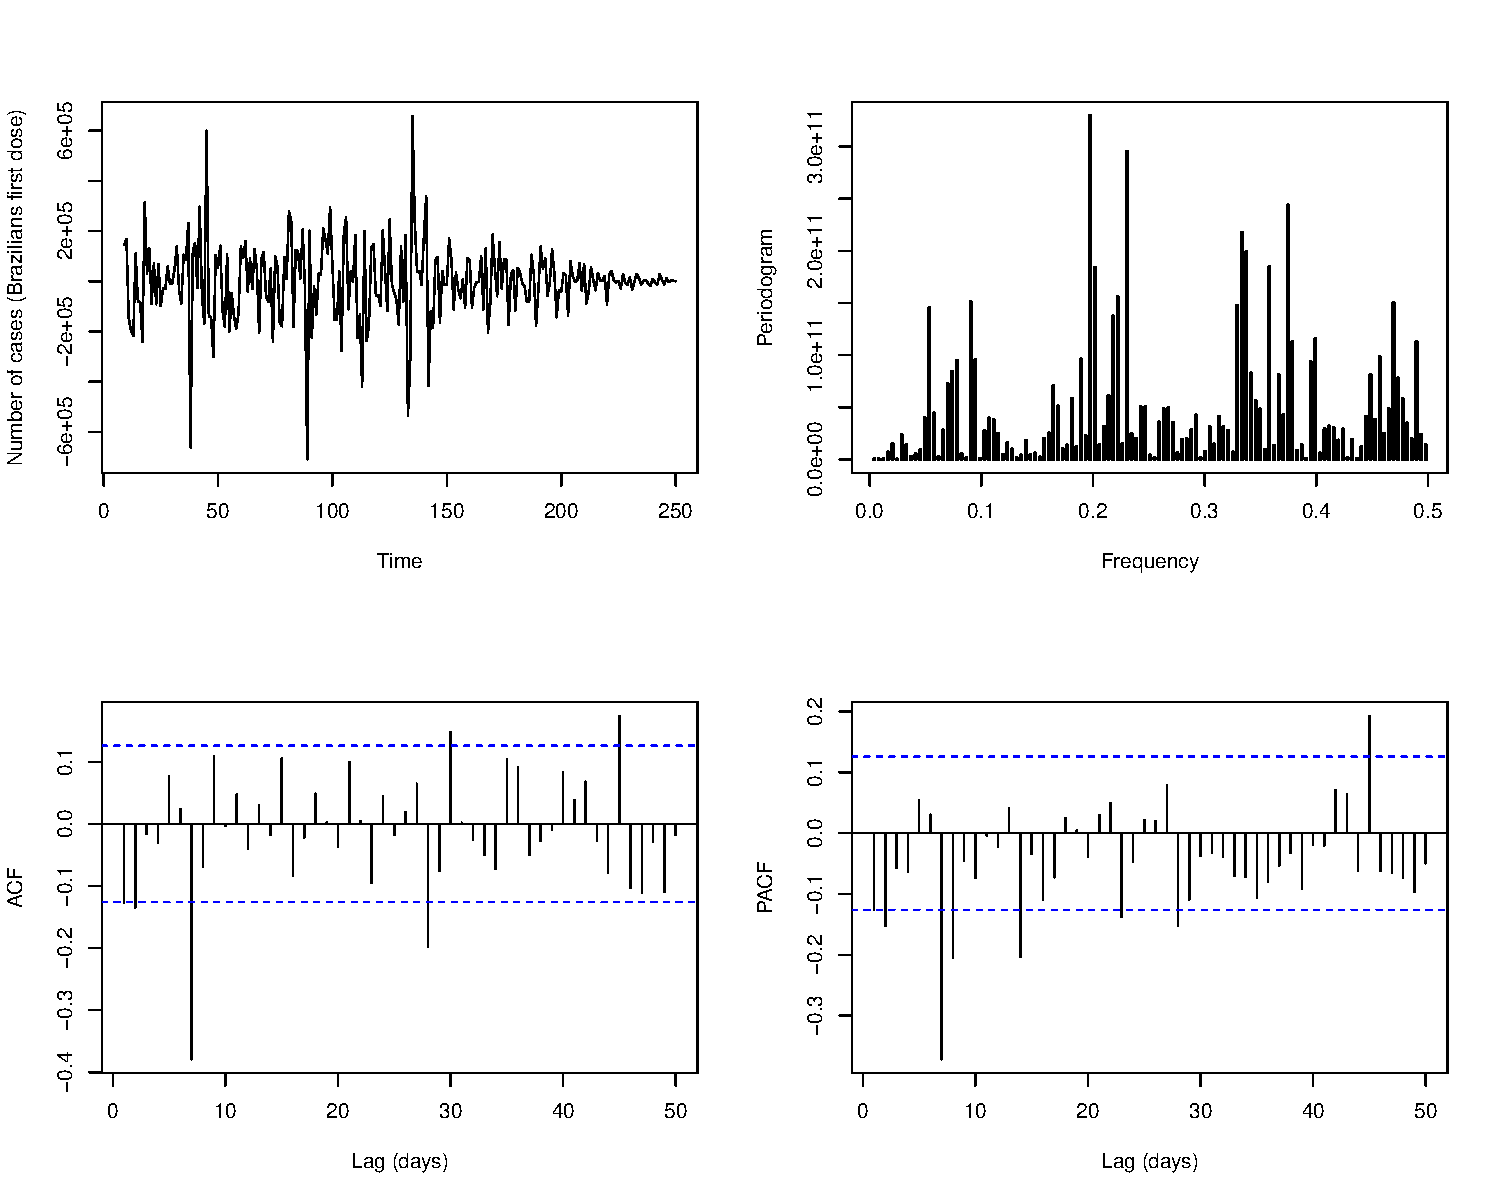
\includegraphics[width=\linewidth]{IF_results_ENG_files/figure-latex/unnamed-chunk-15-1} \end{center}

\textbf{Figure 13}: basic graphs in the analysis of time series applied
to the series of brazilian people vaccinated with the first dose of the
COVID-19 vaccine, considering seasonal differentiation of seven.

Now, we apply the logarithmic transformation to the data.

\begin{Shaded}
\begin{Highlighting}[]
\NormalTok{firstdoseBR\_log }\OtherTok{\textless{}{-}}
  \FunctionTok{log}\NormalTok{(}\FunctionTok{ts}\NormalTok{(series}\SpecialCharTok{$}\NormalTok{first\_dose.BR[start\_vac}\SpecialCharTok{:}\NormalTok{end\_vac]))}
\NormalTok{firstdoseBR\_dif1 }\OtherTok{\textless{}{-}} \FunctionTok{diff}\NormalTok{(firstdoseBR\_log)}
\NormalTok{firstdoseBR\_dif7 }\OtherTok{\textless{}{-}} \FunctionTok{diff}\NormalTok{(firstdoseBR\_dif1, }\DecValTok{7}\NormalTok{)}

\FunctionTok{par}\NormalTok{(}\AttributeTok{mfrow=}\FunctionTok{c}\NormalTok{(}\DecValTok{2}\NormalTok{,}\DecValTok{2}\NormalTok{))}
\FunctionTok{plot.ts}\NormalTok{(firstdoseBR\_dif7,}
        \AttributeTok{xlab =} \StringTok{"Time"}\NormalTok{,}
        \AttributeTok{ylab =} \StringTok{"Number of cases (Brazilians first dose)"}\NormalTok{)}
\NormalTok{TSA}\SpecialCharTok{::}\FunctionTok{periodogram}\NormalTok{(firstdoseBR\_dif7,}
                 \AttributeTok{xlab =} \StringTok{"Frequency"}\NormalTok{,}
                 \AttributeTok{ylab =} \StringTok{"Periodogram"}\NormalTok{)}
\FunctionTok{acf}\NormalTok{(firstdoseBR\_dif7,}
    \AttributeTok{xlab =} \StringTok{"Lag (days)"}\NormalTok{,}
    \AttributeTok{ylab =} \StringTok{"ACF"}\NormalTok{,}
    \AttributeTok{main =} \StringTok{""}\NormalTok{,}
    \AttributeTok{lag.max =} \DecValTok{10}\NormalTok{,}
    \AttributeTok{xaxt =} \StringTok{"n"}\NormalTok{)}
\FunctionTok{axis}\NormalTok{(}\DecValTok{1}\NormalTok{, }\AttributeTok{at =} \DecValTok{1}\SpecialCharTok{:}\DecValTok{10}\NormalTok{)}
\FunctionTok{pacf}\NormalTok{(firstdoseBR\_dif7,}
     \AttributeTok{xlab =} \StringTok{"Lag (days)"}\NormalTok{,}
     \AttributeTok{ylab =} \StringTok{"PACF"}\NormalTok{,}
     \AttributeTok{main =} \StringTok{""}\NormalTok{,}
     \AttributeTok{lag.max =} \DecValTok{10}\NormalTok{,}
     \AttributeTok{xaxt =} \StringTok{"n"}\NormalTok{)}
\FunctionTok{axis}\NormalTok{(}\DecValTok{1}\NormalTok{, }\AttributeTok{at =} \DecValTok{1}\SpecialCharTok{:}\DecValTok{10}\NormalTok{)}
\end{Highlighting}
\end{Shaded}

\begin{center}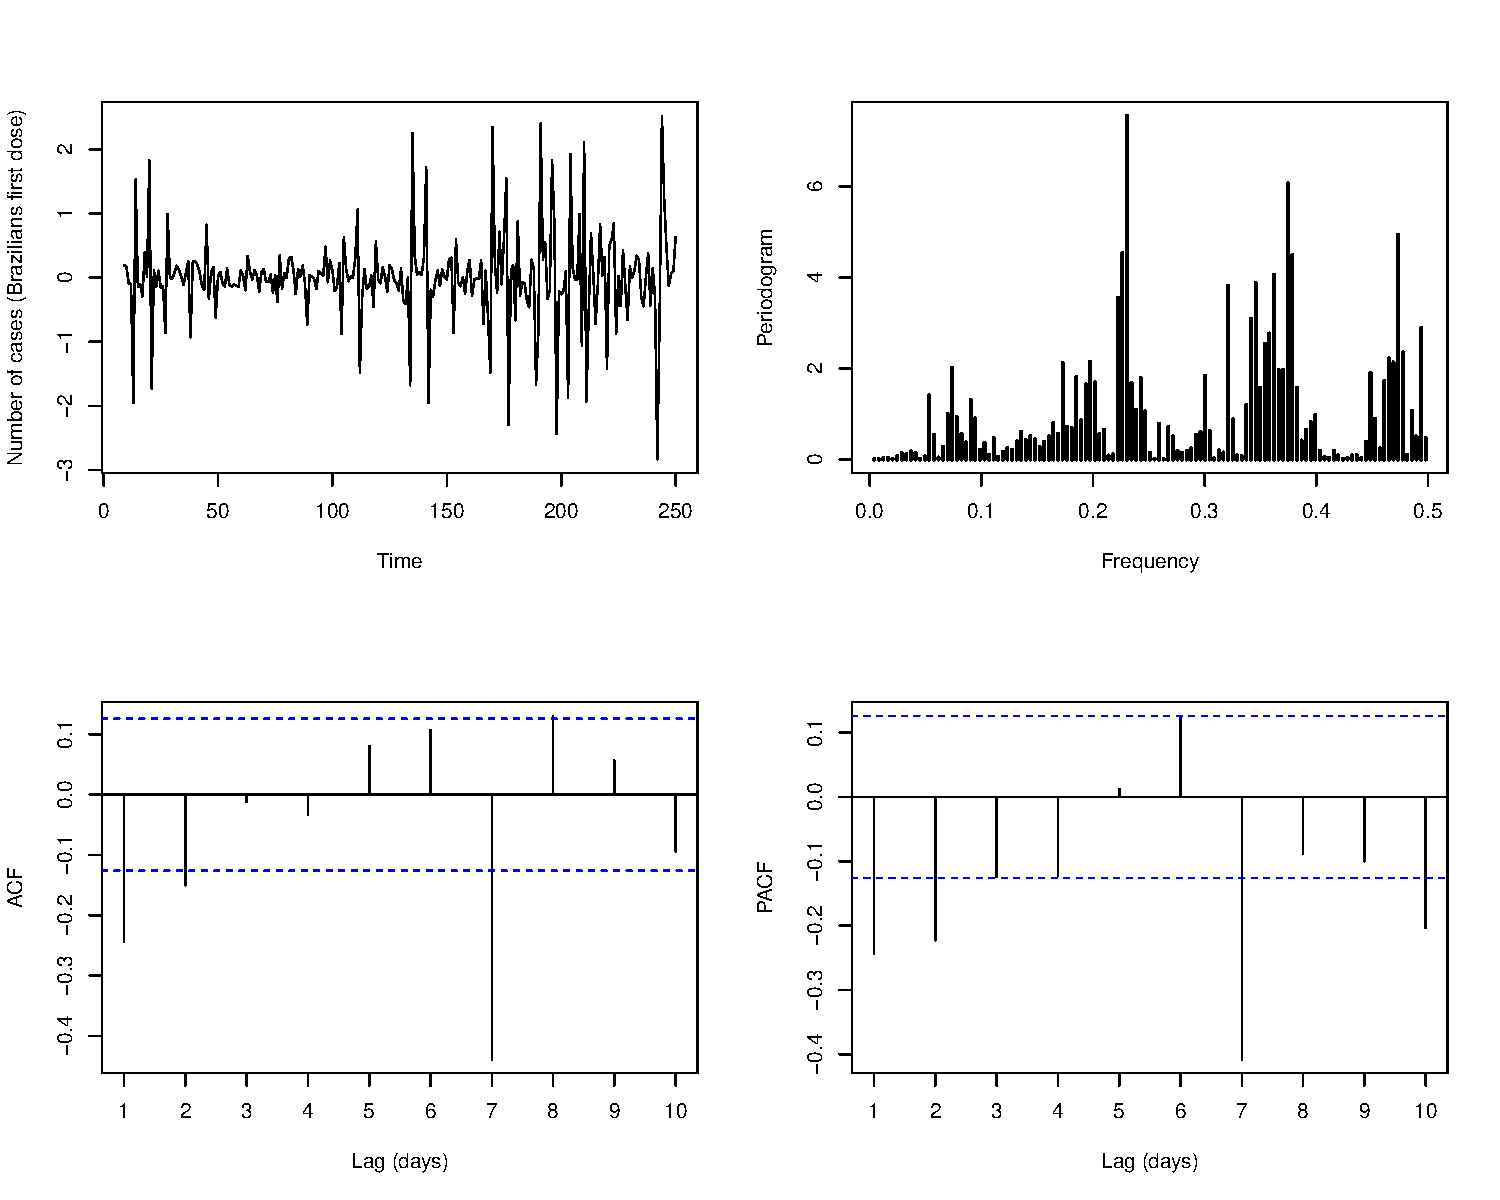
\includegraphics[width=\linewidth]{IF_results_ENG_files/figure-latex/unnamed-chunk-16-1} \end{center}

\textbf{Figure 14}: basic graphs in the analysis of time series applied
to the series of brazilian people vaccinated with the first dose of the
COVID-19 vaccine, considering seasonal differentiation of seven and
logarithmic transformation of the data.

Applying the Augmented Dickey-Fuller Test one more time.

\begin{Shaded}
\begin{Highlighting}[]
\FunctionTok{adf.test}\NormalTok{(firstdoseBR\_dif7)}
\end{Highlighting}
\end{Shaded}

\begin{verbatim}
## 
##  Augmented Dickey-Fuller Test
## 
## data:  firstdoseBR_dif7
## Dickey-Fuller = -9.8798, Lag order = 6, p-value = 0.01
## alternative hypothesis: stationary
\end{verbatim}

Now we have that the time series is stationary.

\subsection{Immunized maternal
population}\label{immunized-maternal-population}

These data consider pregnant and postpartum women who took the second
dose of the vaccine against COVID-19 or a booster dose.

\begin{Shaded}
\begin{Highlighting}[]
\FunctionTok{par}\NormalTok{(}\AttributeTok{mfrow=}\FunctionTok{c}\NormalTok{(}\DecValTok{2}\NormalTok{,}\DecValTok{2}\NormalTok{))}
\FunctionTok{plot.ts}\NormalTok{(}\FunctionTok{ts}\NormalTok{(series}\SpecialCharTok{$}\NormalTok{immunized.GES[start\_vac}\SpecialCharTok{:}\NormalTok{end\_vac]),}
        \AttributeTok{xlab =} \StringTok{"Time"}\NormalTok{,}
        \AttributeTok{ylab =} \StringTok{"Number o cases (immunized)"}\NormalTok{)}
\NormalTok{TSA}\SpecialCharTok{::}\FunctionTok{periodogram}\NormalTok{(}\FunctionTok{ts}\NormalTok{(series}\SpecialCharTok{$}\NormalTok{immunized.GES[start\_vac}\SpecialCharTok{:}\NormalTok{end\_vac]),}
                 \AttributeTok{xlab =} \StringTok{"Frequency"}\NormalTok{,}
                 \AttributeTok{ylab =} \StringTok{"Periodogram"}\NormalTok{)}
\FunctionTok{acf}\NormalTok{(}\FunctionTok{ts}\NormalTok{(series}\SpecialCharTok{$}\NormalTok{immunized.GES[start\_vac}\SpecialCharTok{:}\NormalTok{end\_vac]),}
    \AttributeTok{xlab =} \StringTok{"Lag (days)"}\NormalTok{,}
    \AttributeTok{ylab =} \StringTok{"ACF"}\NormalTok{,}
    \AttributeTok{main =} \StringTok{""}\NormalTok{,}
    \AttributeTok{lag.max =} \DecValTok{250}\NormalTok{)}
\FunctionTok{pacf}\NormalTok{(}\FunctionTok{ts}\NormalTok{(series}\SpecialCharTok{$}\NormalTok{immunized.GES[start\_vac}\SpecialCharTok{:}\NormalTok{end\_vac]),}
     \AttributeTok{xlab =} \StringTok{"Lag (days)"}\NormalTok{,}
     \AttributeTok{ylab =} \StringTok{"PACF"}\NormalTok{,}
     \AttributeTok{main =} \StringTok{""}\NormalTok{,}
     \AttributeTok{lag.max =} \DecValTok{250}\NormalTok{)}
\end{Highlighting}
\end{Shaded}

\begin{center}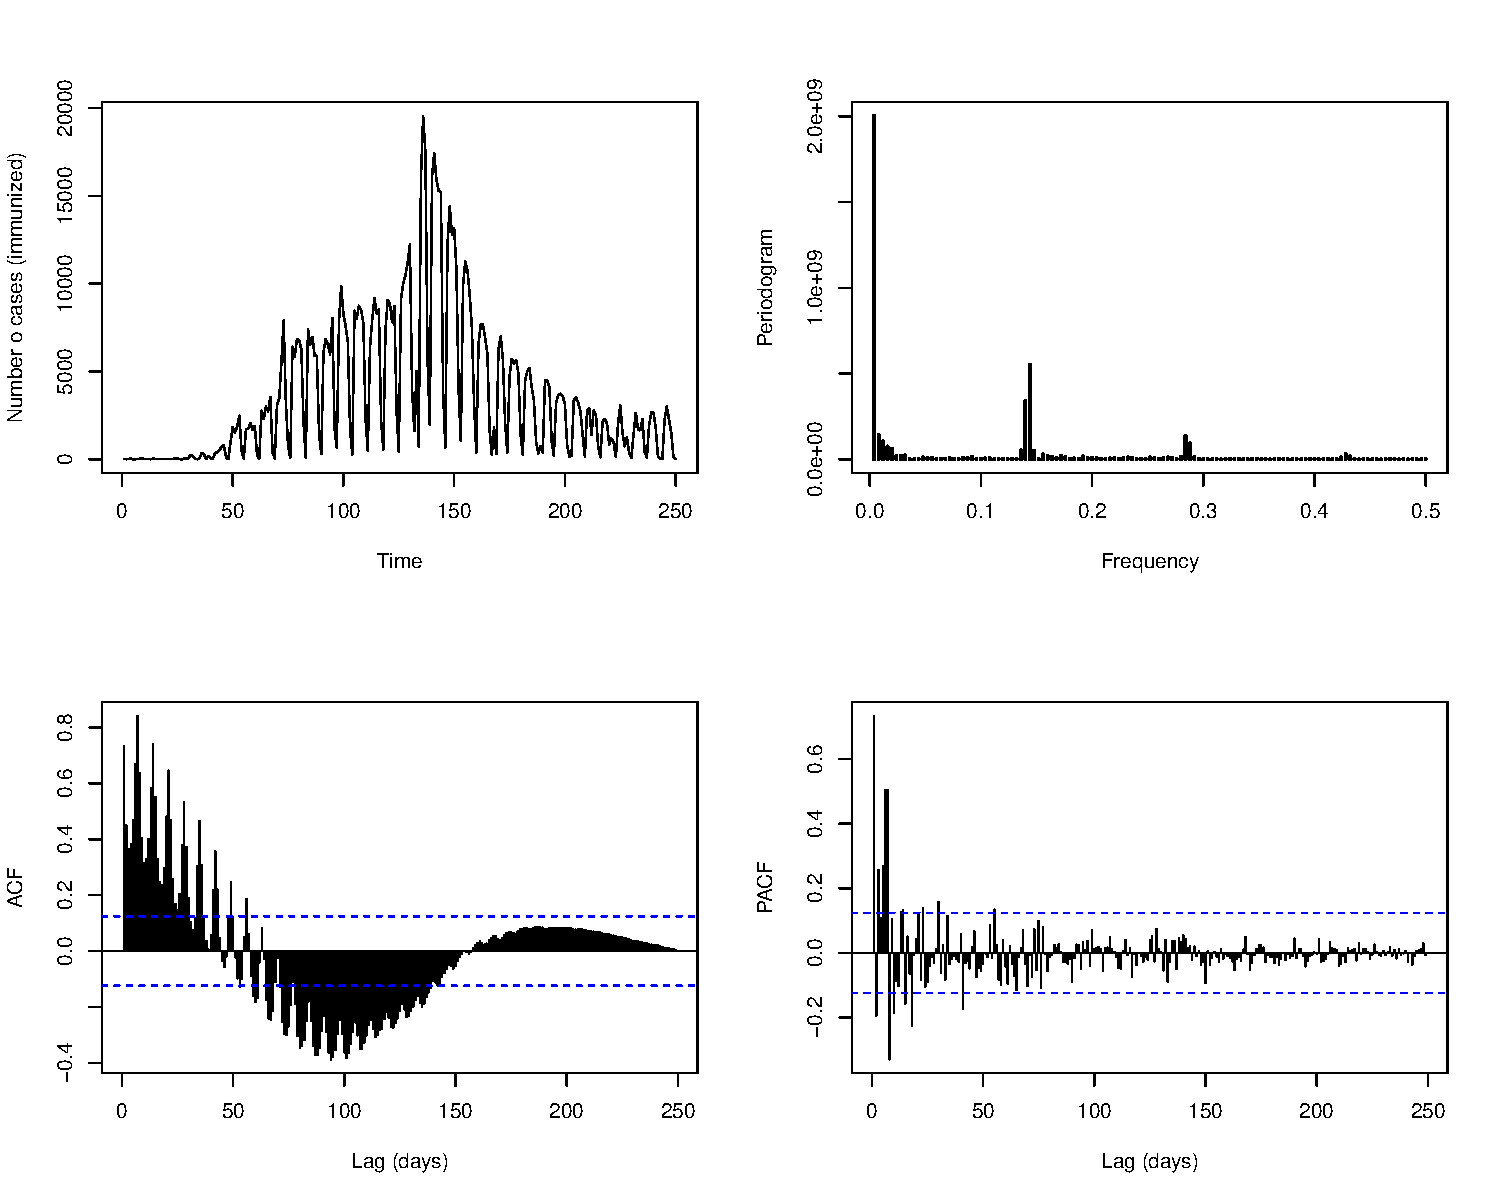
\includegraphics[width=\linewidth]{IF_results_ENG_files/figure-latex/unnamed-chunk-18-1} \end{center}

\textbf{Figure 15}: basic graphs in the analysis of time series applied
to the series of immunized maternal population.

We clearly see that the time series of immunized pregnant women is not
stationary as the mean and variance seems to be non-constant. Also, we
can notice jumps through the bars when we look at the autocorrelation
and periodogram graphs, which suggests that maybe there is a cicle to be
considered.

Checking the non-stationarity assumption of the time series.

\begin{Shaded}
\begin{Highlighting}[]
\FunctionTok{adf.test}\NormalTok{(}\FunctionTok{ts}\NormalTok{(series}\SpecialCharTok{$}\NormalTok{immunized.GES[start\_vac}\SpecialCharTok{:}\NormalTok{end\_vac]))}
\end{Highlighting}
\end{Shaded}

\begin{verbatim}
## 
##  Augmented Dickey-Fuller Test
## 
## data:  ts(series$immunized.GES[start_vac:end_vac])
## Dickey-Fuller = -0.81152, Lag order = 6, p-value = 0.9597
## alternative hypothesis: stationary
\end{verbatim}

Let's apply 1 differentiation and verify the time series.

\begin{Shaded}
\begin{Highlighting}[]
\DocumentationTok{\#\# 1 differentiation}
\NormalTok{immunized\_dif1 }\OtherTok{\textless{}{-}} \FunctionTok{diff}\NormalTok{(}\FunctionTok{ts}\NormalTok{(series}\SpecialCharTok{$}\NormalTok{immunized.GES[start\_vac}\SpecialCharTok{:}\NormalTok{end\_vac]))}

\FunctionTok{par}\NormalTok{(}\AttributeTok{mfrow=}\FunctionTok{c}\NormalTok{(}\DecValTok{2}\NormalTok{,}\DecValTok{2}\NormalTok{))}
\FunctionTok{plot.ts}\NormalTok{(immunized\_dif1,}
        \AttributeTok{xlab =} \StringTok{"Time"}\NormalTok{,}
        \AttributeTok{ylab =} \StringTok{"Number of cases (immunized)"}\NormalTok{)}
\NormalTok{TSA}\SpecialCharTok{::}\FunctionTok{periodogram}\NormalTok{(immunized\_dif1,}
                 \AttributeTok{xlab =} \StringTok{"Frequency"}\NormalTok{,}
                 \AttributeTok{ylab =} \StringTok{"Periodogram"}\NormalTok{)}
\FunctionTok{acf}\NormalTok{(immunized\_dif1,}
    \AttributeTok{xlab =} \StringTok{"Lag (days)"}\NormalTok{,}
    \AttributeTok{ylab =} \StringTok{"ACF"}\NormalTok{,}
    \AttributeTok{main =} \StringTok{""}\NormalTok{,}
    \AttributeTok{lag.max =} \DecValTok{50}\NormalTok{)}
\FunctionTok{pacf}\NormalTok{(immunized\_dif1,}
     \AttributeTok{xlab =} \StringTok{"Lag (days)"}\NormalTok{,}
     \AttributeTok{ylab =} \StringTok{"PACF"}\NormalTok{,}
     \AttributeTok{main =} \StringTok{""}\NormalTok{,}
     \AttributeTok{lag.max =} \DecValTok{50}\NormalTok{)}
\end{Highlighting}
\end{Shaded}

\begin{center}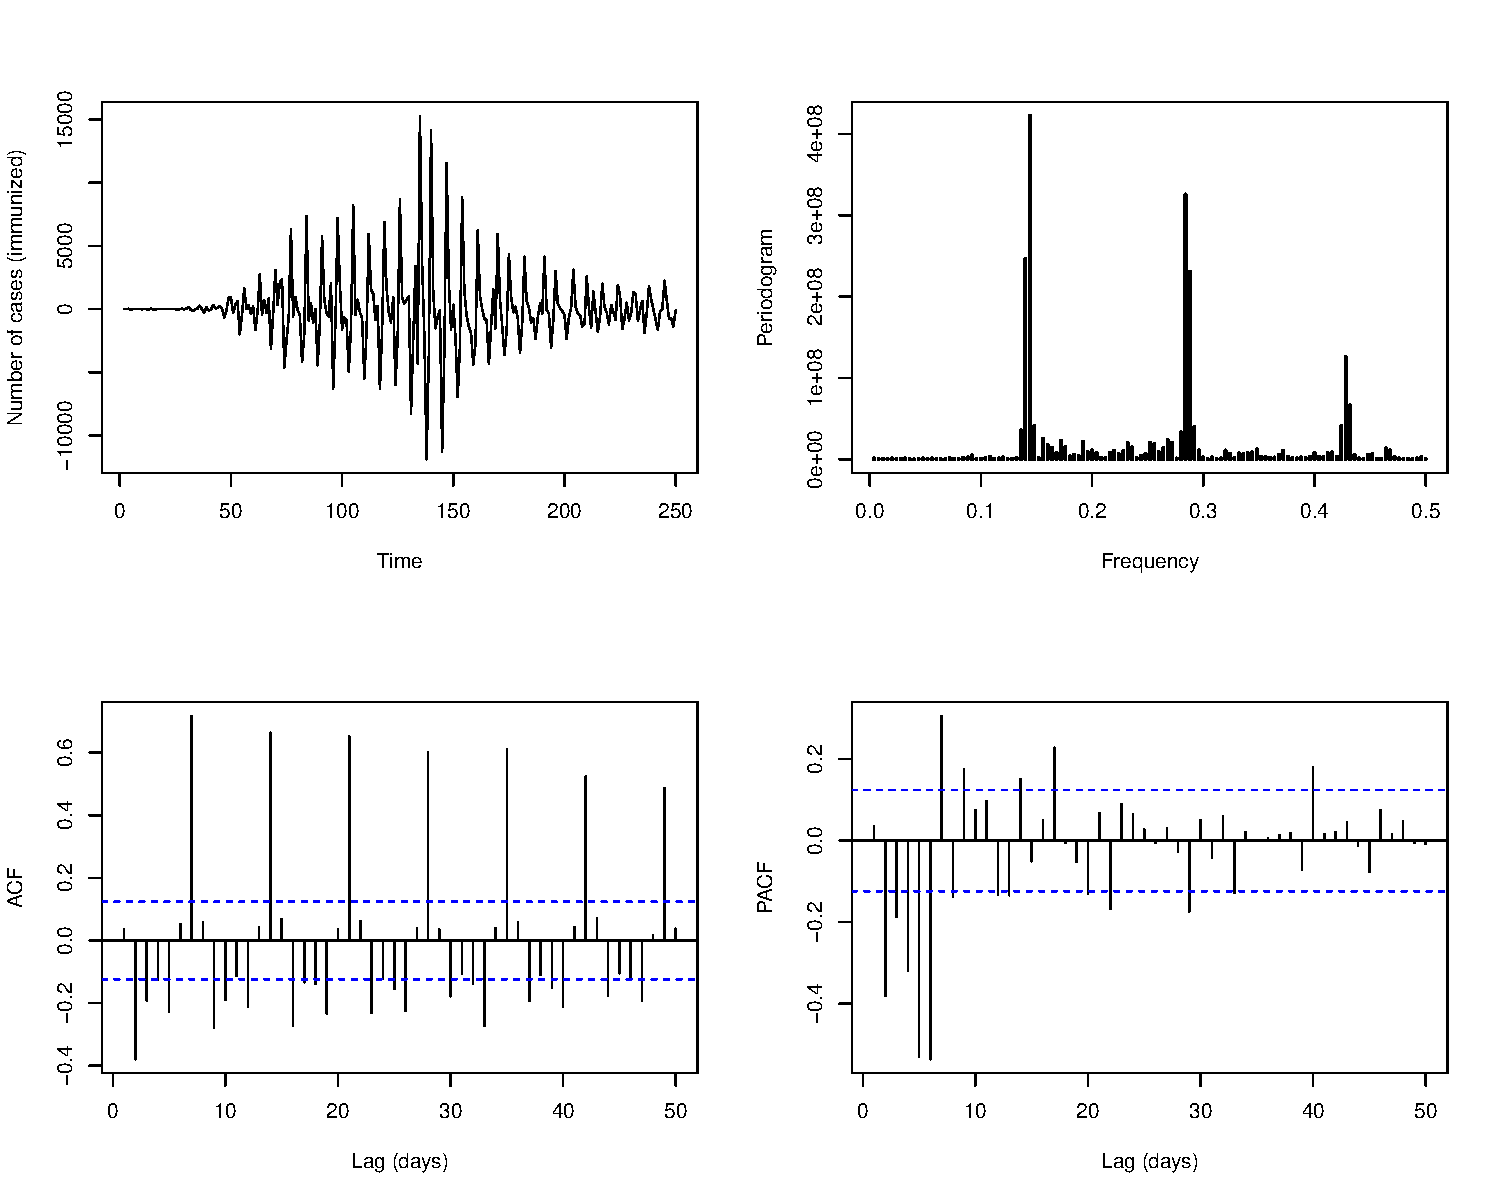
\includegraphics[width=\linewidth]{IF_results_ENG_files/figure-latex/unnamed-chunk-20-1} \end{center}

\textbf{Figure 16}: basic graphs in the analysis of time series applied
to the series of immunized maternal population, considering one
differentiation.

We can see that the jumps between the bars are now more evident, and we
can see a period of 7 days when we look at the autocorrelation graph.
Now, we need to inform this cycle in the differentiation process.

\begin{Shaded}
\begin{Highlighting}[]
\NormalTok{immunized\_dif7 }\OtherTok{\textless{}{-}}
  \FunctionTok{diff}\NormalTok{(}\FunctionTok{ts}\NormalTok{(immunized\_dif1), }\DecValTok{7}\NormalTok{)}

\FunctionTok{par}\NormalTok{(}\AttributeTok{mfrow=}\FunctionTok{c}\NormalTok{(}\DecValTok{2}\NormalTok{,}\DecValTok{2}\NormalTok{))}
\FunctionTok{plot.ts}\NormalTok{(immunized\_dif7,}
        \AttributeTok{xlab =} \StringTok{"Time"}\NormalTok{,}
        \AttributeTok{ylab =} \StringTok{"Number of cases (immunized)"}\NormalTok{)}
\NormalTok{TSA}\SpecialCharTok{::}\FunctionTok{periodogram}\NormalTok{(immunized\_dif7,}
                 \AttributeTok{xlab =} \StringTok{"Frequency"}\NormalTok{,}
                 \AttributeTok{ylab =} \StringTok{"Periodogram"}\NormalTok{)}
\FunctionTok{acf}\NormalTok{(immunized\_dif7,}
    \AttributeTok{xlab =} \StringTok{"Lag (days)"}\NormalTok{,}
    \AttributeTok{ylab =} \StringTok{"ACF"}\NormalTok{,}
    \AttributeTok{main =} \StringTok{""}\NormalTok{,}
    \AttributeTok{lag.max =} \DecValTok{50}\NormalTok{)}
\FunctionTok{pacf}\NormalTok{(immunized\_dif7,}
     \AttributeTok{xlab =} \StringTok{"Lag (days)"}\NormalTok{,}
     \AttributeTok{ylab =} \StringTok{"PACF"}\NormalTok{,}
     \AttributeTok{main =} \StringTok{""}\NormalTok{,}
     \AttributeTok{lag.max =} \DecValTok{50}\NormalTok{)}
\end{Highlighting}
\end{Shaded}

\begin{center}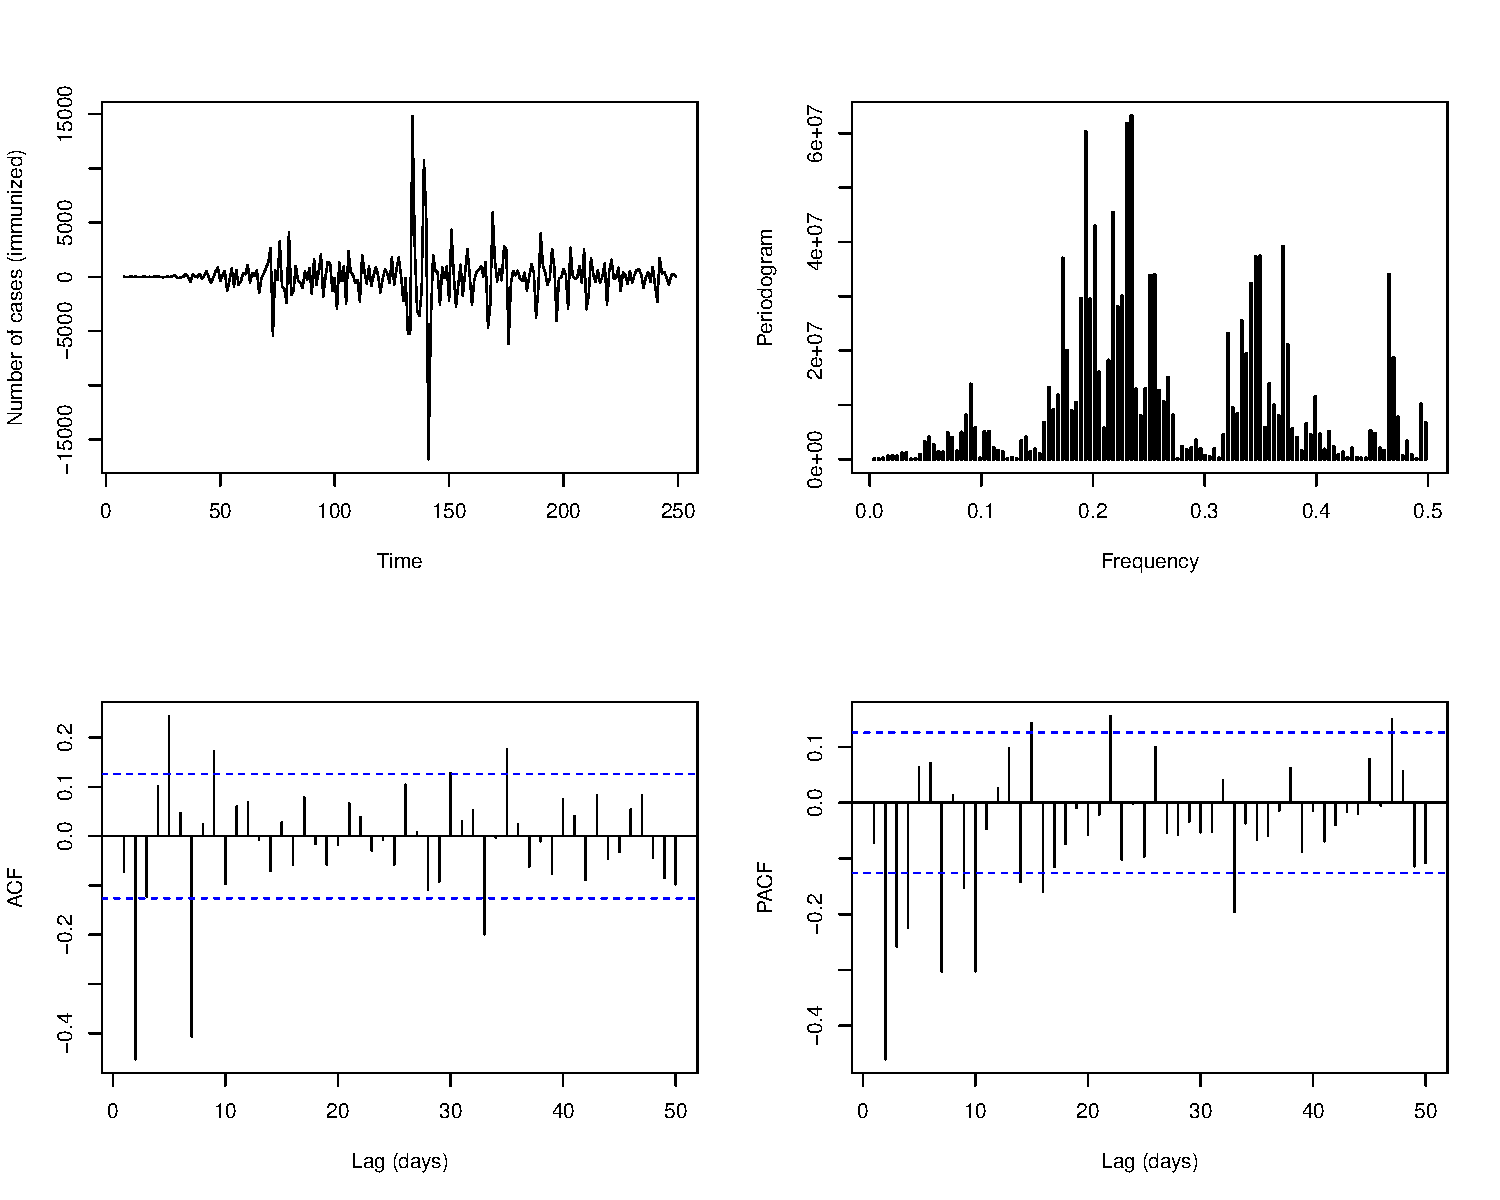
\includegraphics[width=\linewidth]{IF_results_ENG_files/figure-latex/unnamed-chunk-21-1} \end{center}

\textbf{Figure 17}: basic graphs in the analysis of time series applied
to the series of immunized maternal population, considering seasonal
differentiation of seven.

Now, we apply the data transformation.

\begin{Shaded}
\begin{Highlighting}[]
\DocumentationTok{\#\# Summary of the time series}
\FunctionTok{summary}\NormalTok{(}\FunctionTok{ts}\NormalTok{(series}\SpecialCharTok{$}\NormalTok{immunized.GES[start\_vac}\SpecialCharTok{:}\NormalTok{end\_vac]))}
\end{Highlighting}
\end{Shaded}

\begin{verbatim}
##    Min. 1st Qu.  Median    Mean 3rd Qu.    Max. 
##     0.0   280.2  2052.0  3568.7  5949.0 19552.0
\end{verbatim}

\begin{Shaded}
\begin{Highlighting}[]
\DocumentationTok{\#\# \#\# Adding 3500}
\NormalTok{immunized\_log }\OtherTok{\textless{}{-}}
  \FunctionTok{log}\NormalTok{(}\FunctionTok{ts}\NormalTok{(series}\SpecialCharTok{$}\NormalTok{immunized.GES[start\_vac}\SpecialCharTok{:}\NormalTok{end\_vac]) }\SpecialCharTok{+} \DecValTok{3500}\NormalTok{)}
\NormalTok{immunized\_log\_dif1 }\OtherTok{\textless{}{-}} \FunctionTok{diff}\NormalTok{(immunized\_log)}
\NormalTok{immunized\_dif7 }\OtherTok{\textless{}{-}} \FunctionTok{diff}\NormalTok{(immunized\_log\_dif1, }\DecValTok{7}\NormalTok{)}

\FunctionTok{par}\NormalTok{(}\AttributeTok{mfrow=}\FunctionTok{c}\NormalTok{(}\DecValTok{2}\NormalTok{,}\DecValTok{2}\NormalTok{))}
\FunctionTok{plot.ts}\NormalTok{(immunized\_dif7,}
        \AttributeTok{xlab =} \StringTok{"Time"}\NormalTok{,}
        \AttributeTok{ylab =} \StringTok{"Number of cases (immunized)"}\NormalTok{)}
\NormalTok{TSA}\SpecialCharTok{::}\FunctionTok{periodogram}\NormalTok{(immunized\_dif7,}
                 \AttributeTok{xlab =} \StringTok{"Frequency"}\NormalTok{,}
                 \AttributeTok{ylab =} \StringTok{"Periodogram"}\NormalTok{)}
\FunctionTok{acf}\NormalTok{(immunized\_dif7,}
    \AttributeTok{xlab =} \StringTok{"Lag (days)"}\NormalTok{,}
    \AttributeTok{ylab =} \StringTok{"ACF"}\NormalTok{,}
    \AttributeTok{main =} \StringTok{""}\NormalTok{,}
    \AttributeTok{lag.max =} \DecValTok{10}\NormalTok{,}
    \AttributeTok{xaxt =} \StringTok{"n"}\NormalTok{)}
\FunctionTok{axis}\NormalTok{(}\DecValTok{1}\NormalTok{, }\AttributeTok{at =} \DecValTok{1}\SpecialCharTok{:}\DecValTok{10}\NormalTok{)}
\FunctionTok{pacf}\NormalTok{(immunized\_dif7,}
     \AttributeTok{xlab =} \StringTok{"Lag (days)"}\NormalTok{,}
     \AttributeTok{ylab =} \StringTok{"PACF"}\NormalTok{,}
     \AttributeTok{main =} \StringTok{""}\NormalTok{,}
     \AttributeTok{lag.max =} \DecValTok{10}\NormalTok{,}
     \AttributeTok{xaxt =} \StringTok{"n"}\NormalTok{)}
\FunctionTok{axis}\NormalTok{(}\DecValTok{1}\NormalTok{, }\AttributeTok{at =} \DecValTok{1}\SpecialCharTok{:}\DecValTok{10}\NormalTok{)}
\end{Highlighting}
\end{Shaded}

\begin{center}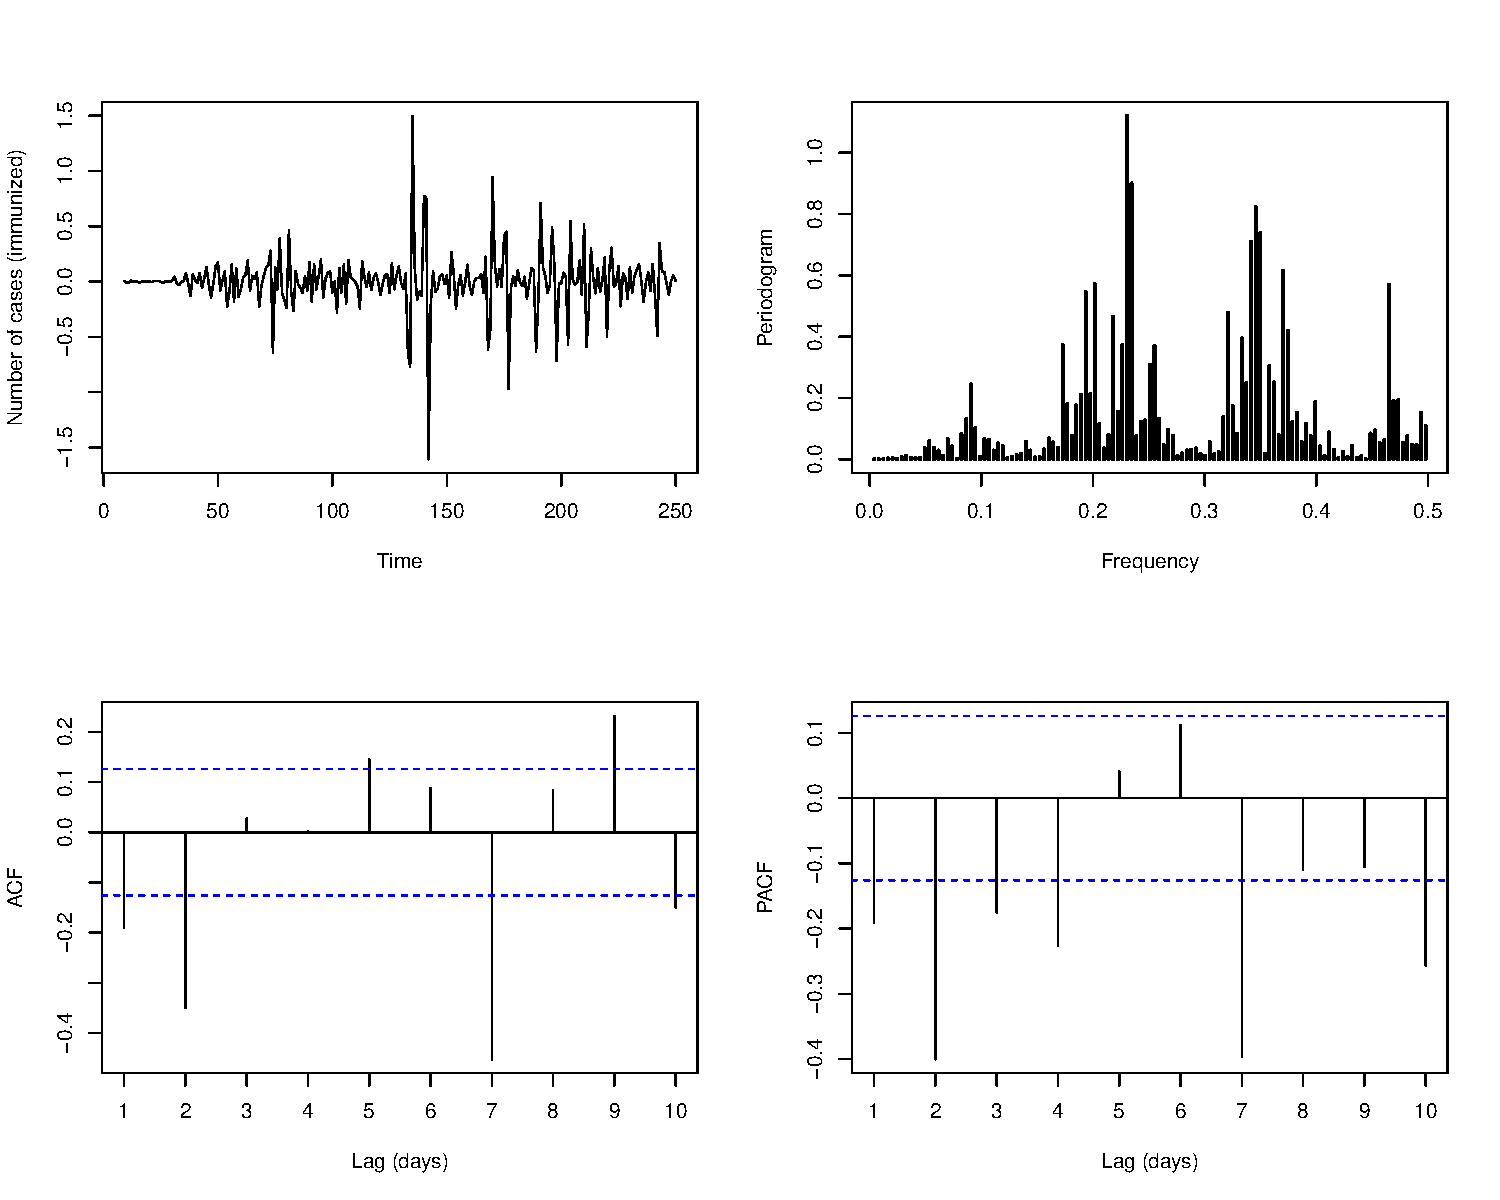
\includegraphics[width=\linewidth]{IF_results_ENG_files/figure-latex/unnamed-chunk-22-1} \end{center}

\textbf{Figure 18}: basic graphs in the analysis of time series applied
to the series of immunized maternal population, considering seasonal
differentiation of seven and logarithmic transformation of the data
adding the mean.

Now, we verify one more time if the time series is stationary.

\begin{Shaded}
\begin{Highlighting}[]
\FunctionTok{adf.test}\NormalTok{(immunized\_dif7)}
\end{Highlighting}
\end{Shaded}

\begin{verbatim}
## 
##  Augmented Dickey-Fuller Test
## 
## data:  immunized_dif7
## Dickey-Fuller = -9.7464, Lag order = 6, p-value = 0.01
## alternative hypothesis: stationary
\end{verbatim}

The Augmented Dickey-Fuller Test points out that the series is
stationary.

\subsection{Immunized brazilian
population}\label{immunized-brazilian-population}

These data consider brazilians in general who took the second dose of
the vaccine against COVID-19 or a booster dose.

First, we analyze the basic graphs of the time series.

\begin{Shaded}
\begin{Highlighting}[]
\FunctionTok{par}\NormalTok{(}\AttributeTok{mfrow=}\FunctionTok{c}\NormalTok{(}\DecValTok{2}\NormalTok{,}\DecValTok{2}\NormalTok{))}
\FunctionTok{plot.ts}\NormalTok{(}\FunctionTok{ts}\NormalTok{(series}\SpecialCharTok{$}\NormalTok{immunized.BR[start\_vac}\SpecialCharTok{:}\NormalTok{end\_vac]),}
        \AttributeTok{xlab =} \StringTok{"Time"}\NormalTok{,}
        \AttributeTok{ylab =} \StringTok{"Number of cases (Immunized Brazilian People)"}\NormalTok{)}

\NormalTok{TSA}\SpecialCharTok{::}\FunctionTok{periodogram}\NormalTok{(}\FunctionTok{ts}\NormalTok{(series}\SpecialCharTok{$}\NormalTok{immunized.BR[start\_vac}\SpecialCharTok{:}\NormalTok{end\_vac]),}
                 \AttributeTok{xlab =} \StringTok{"Frequency"}\NormalTok{,}
                 \AttributeTok{ylab =} \StringTok{"Periodogram"}\NormalTok{)}
\FunctionTok{acf}\NormalTok{(}\FunctionTok{ts}\NormalTok{(series}\SpecialCharTok{$}\NormalTok{immunized.BR[start\_vac}\SpecialCharTok{:}\NormalTok{end\_vac]),}
    \AttributeTok{xlab =} \StringTok{"Lag (days)"}\NormalTok{,}
    \AttributeTok{ylab =} \StringTok{"ACF"}\NormalTok{,}
    \AttributeTok{main =} \StringTok{""}\NormalTok{,}
    \AttributeTok{lag.max =} \DecValTok{250}\NormalTok{)}
\FunctionTok{pacf}\NormalTok{(}\FunctionTok{ts}\NormalTok{(series}\SpecialCharTok{$}\NormalTok{immunized.BR[start\_vac}\SpecialCharTok{:}\NormalTok{end\_vac]),}
     \AttributeTok{xlab =} \StringTok{"Lag (days)"}\NormalTok{,}
     \AttributeTok{ylab =} \StringTok{"PACF"}\NormalTok{,}
     \AttributeTok{main =} \StringTok{""}\NormalTok{,}
     \AttributeTok{lag.max =} \DecValTok{250}\NormalTok{)}
\end{Highlighting}
\end{Shaded}

\begin{center}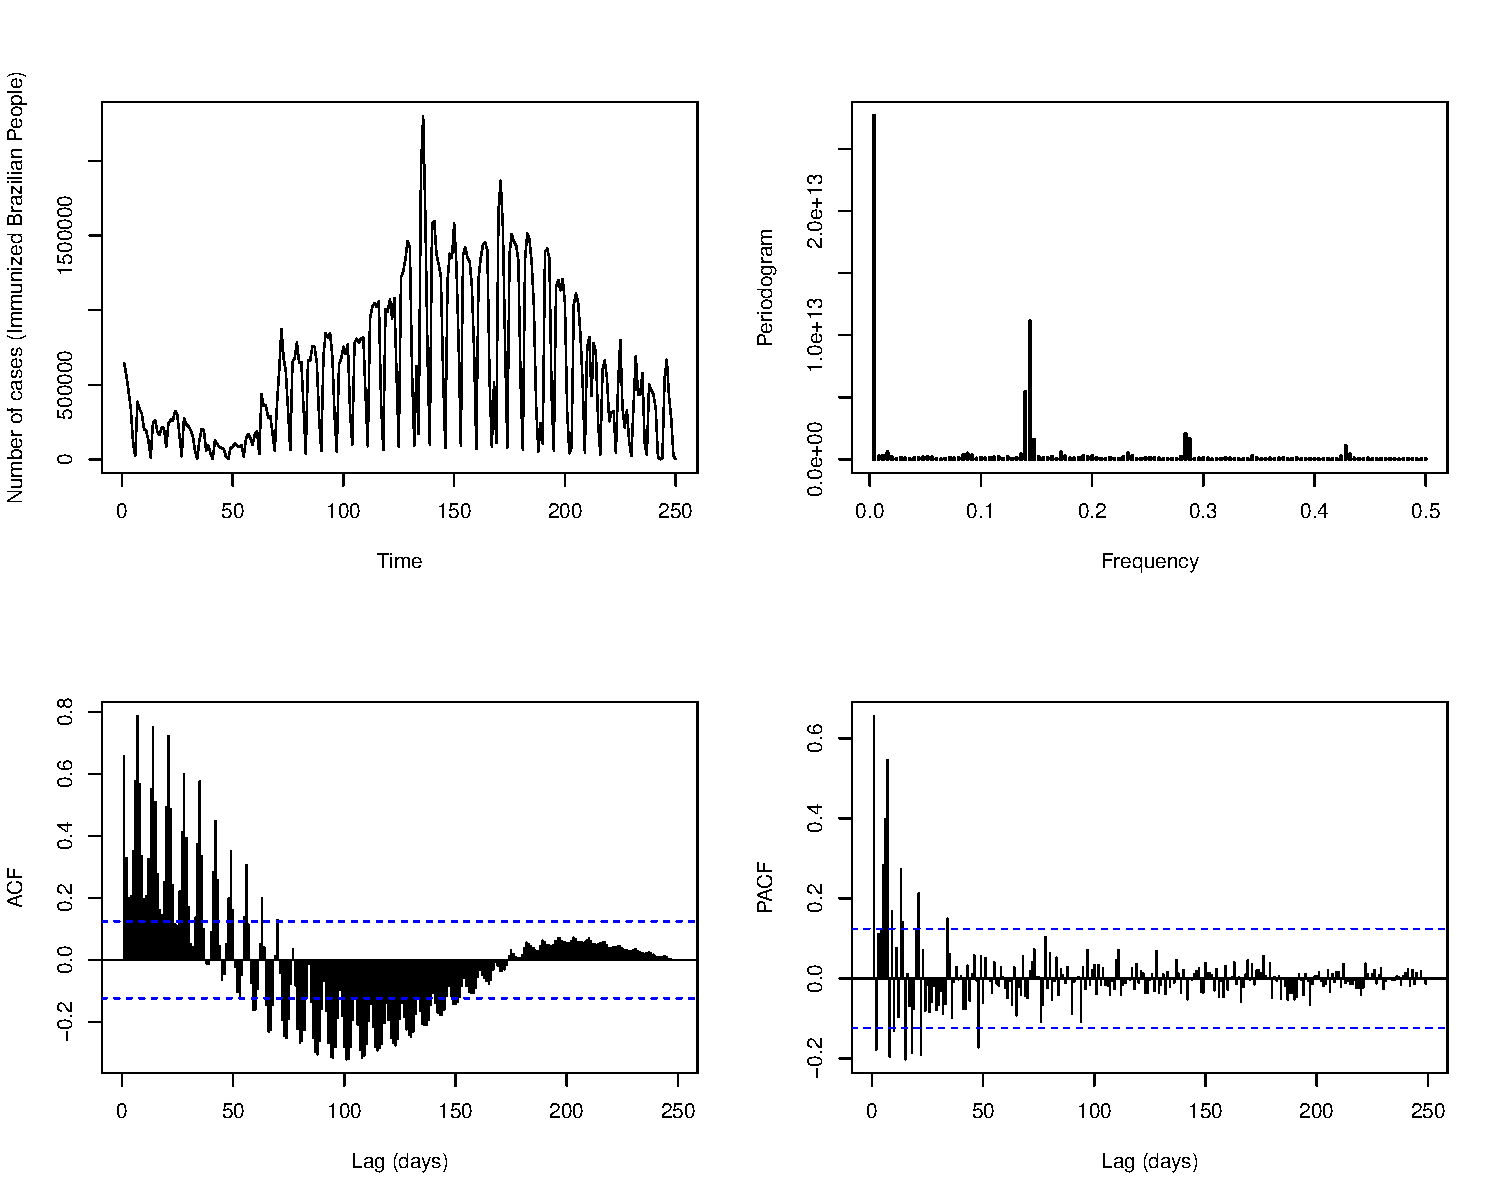
\includegraphics[width=\linewidth]{IF_results_ENG_files/figure-latex/unnamed-chunk-24-1} \end{center}

\textbf{Figure 19}: basic graphs in the analysis of time series applied
to the series of immunized brazilian population.

The time series seems to be not stationary, as the mean and the variance
looks not constant over time. We also can notice jumps through the bars
in the autocorrelation and periodogram graphs. Let's try to apply one
differentiation.

\begin{Shaded}
\begin{Highlighting}[]
\DocumentationTok{\#\# 1 differentiation}
\NormalTok{immunizedBR\_dif1 }\OtherTok{\textless{}{-}} \FunctionTok{diff}\NormalTok{(}\FunctionTok{ts}\NormalTok{(series}\SpecialCharTok{$}\NormalTok{immunized.BR[start\_vac}\SpecialCharTok{:}\NormalTok{end\_vac]))}

\FunctionTok{par}\NormalTok{(}\AttributeTok{mfrow=}\FunctionTok{c}\NormalTok{(}\DecValTok{2}\NormalTok{,}\DecValTok{2}\NormalTok{))}
\FunctionTok{plot.ts}\NormalTok{(immunizedBR\_dif1,}
        \AttributeTok{xlab =} \StringTok{"Time"}\NormalTok{,}
        \AttributeTok{ylab =} \StringTok{"Number of cases (Immunized Brazilian People)"}\NormalTok{)}
\NormalTok{TSA}\SpecialCharTok{::}\FunctionTok{periodogram}\NormalTok{(immunizedBR\_dif1,}
                 \AttributeTok{xlab =} \StringTok{"Frequency"}\NormalTok{,}
                 \AttributeTok{ylab =} \StringTok{"Periodogram"}\NormalTok{)}
\FunctionTok{acf}\NormalTok{(immunizedBR\_dif1,}
    \AttributeTok{xlab =} \StringTok{"Lag (days)"}\NormalTok{,}
    \AttributeTok{ylab =} \StringTok{"ACF"}\NormalTok{,}
    \AttributeTok{main =} \StringTok{""}\NormalTok{,}
    \AttributeTok{lag.max =} \DecValTok{50}\NormalTok{)}
\FunctionTok{pacf}\NormalTok{(immunizedBR\_dif1,}
     \AttributeTok{xlab =} \StringTok{"Lag (days)"}\NormalTok{,}
     \AttributeTok{ylab =} \StringTok{"PACF"}\NormalTok{,}
     \AttributeTok{main =} \StringTok{""}\NormalTok{,}
     \AttributeTok{lag.max =} \DecValTok{50}\NormalTok{)}
\end{Highlighting}
\end{Shaded}

\begin{center}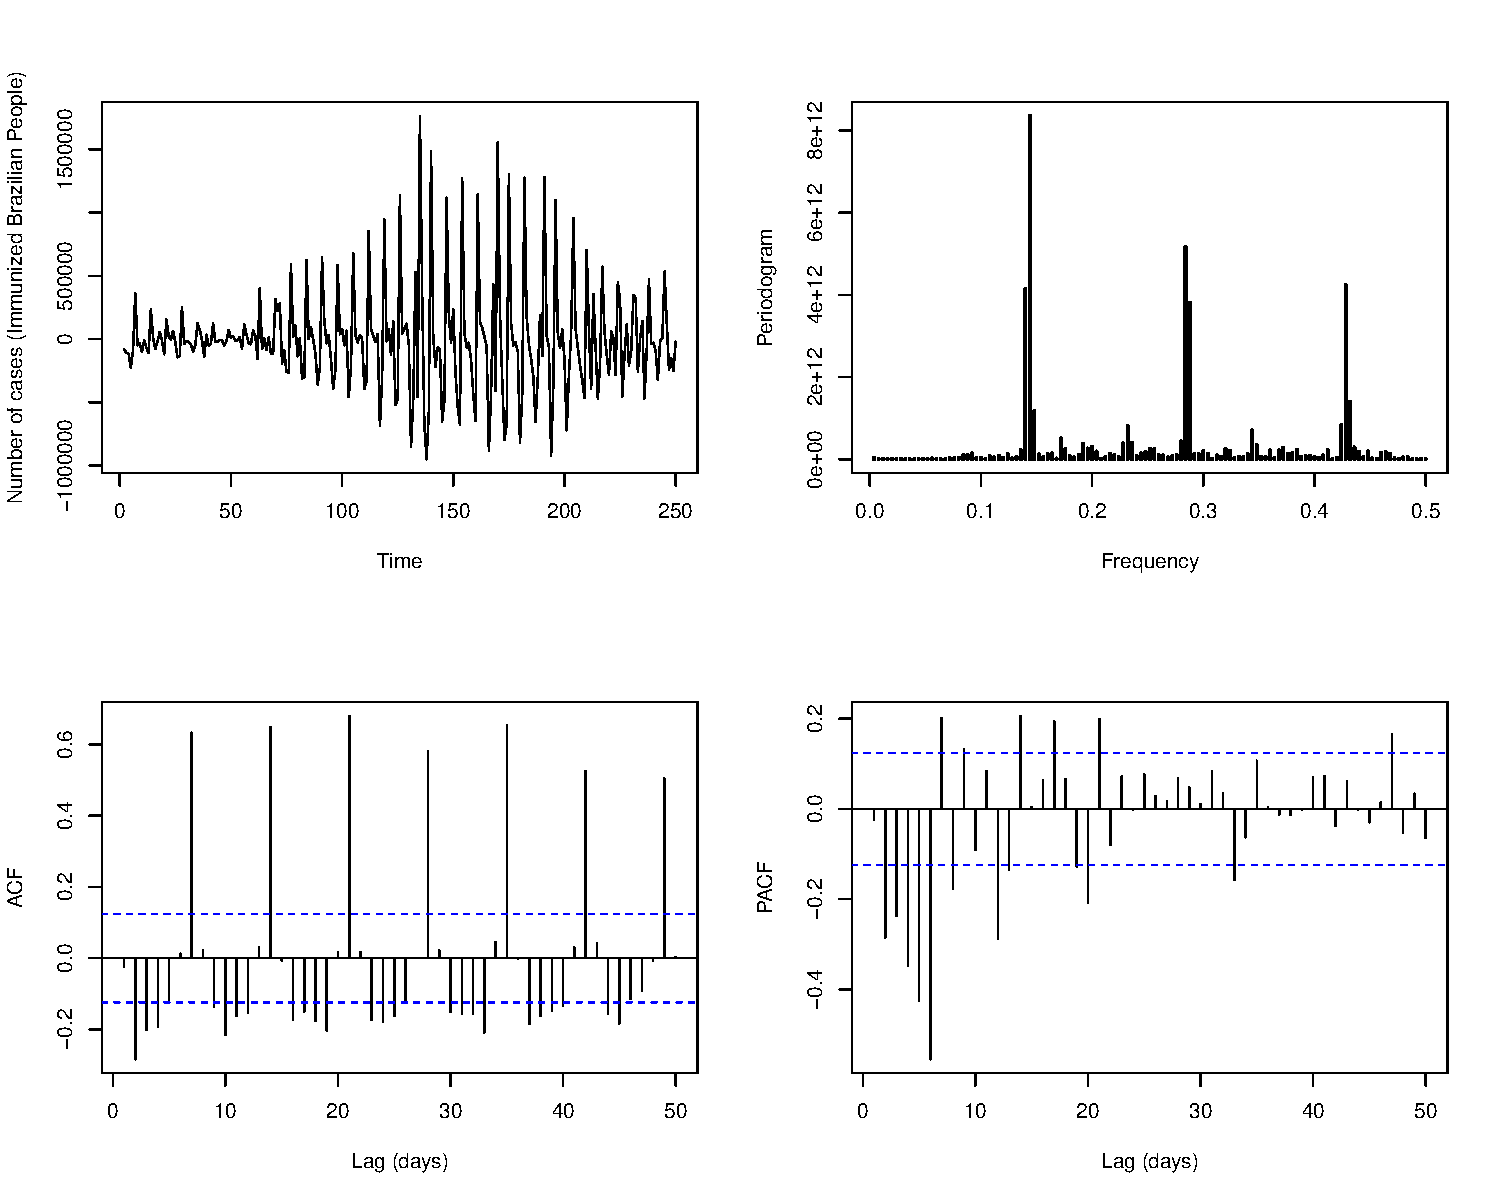
\includegraphics[width=\linewidth]{IF_results_ENG_files/figure-latex/unnamed-chunk-25-1} \end{center}

\textbf{Figure 20}: basic graphs in the analysis of time series applied
to the series of immunized brazilian population considering one
differentiation.

The jumps between the bars of the autocorrelation and periodogram graphs
became more evident after the differentiation, now we can notice a
period of 7 days as in the previous time series. We need to inform this
period in the differentiation process.

\begin{Shaded}
\begin{Highlighting}[]
\NormalTok{immunizedBR\_dif7 }\OtherTok{\textless{}{-}} \FunctionTok{diff}\NormalTok{(immunizedBR\_dif1, }\DecValTok{7}\NormalTok{)}

\FunctionTok{par}\NormalTok{(}\AttributeTok{mfrow=}\FunctionTok{c}\NormalTok{(}\DecValTok{2}\NormalTok{,}\DecValTok{2}\NormalTok{))}
\FunctionTok{plot.ts}\NormalTok{(immunizedBR\_dif7,}
        \AttributeTok{xlab =} \StringTok{"Time"}\NormalTok{,}
        \AttributeTok{ylab =} \StringTok{"Number of cases (Immunized Brazilian People)"}\NormalTok{)}
\NormalTok{TSA}\SpecialCharTok{::}\FunctionTok{periodogram}\NormalTok{(immunizedBR\_dif7,}
                 \AttributeTok{xlab =} \StringTok{"Frequency"}\NormalTok{,}
                 \AttributeTok{ylab =} \StringTok{"Periodogram"}\NormalTok{)}
\FunctionTok{acf}\NormalTok{(immunizedBR\_dif7,}
    \AttributeTok{xlab =} \StringTok{"Lag (days)"}\NormalTok{,}
    \AttributeTok{ylab =} \StringTok{"ACF"}\NormalTok{,}
    \AttributeTok{main =} \StringTok{""}\NormalTok{,}
    \AttributeTok{lag.max =} \DecValTok{50}\NormalTok{)}
\FunctionTok{pacf}\NormalTok{(immunizedBR\_dif7,}
     \AttributeTok{xlab =} \StringTok{"Lag (days)"}\NormalTok{,}
     \AttributeTok{ylab =} \StringTok{"PACF"}\NormalTok{,}
     \AttributeTok{main =} \StringTok{""}\NormalTok{,}
     \AttributeTok{lag.max =} \DecValTok{50}\NormalTok{)}
\end{Highlighting}
\end{Shaded}

\begin{center}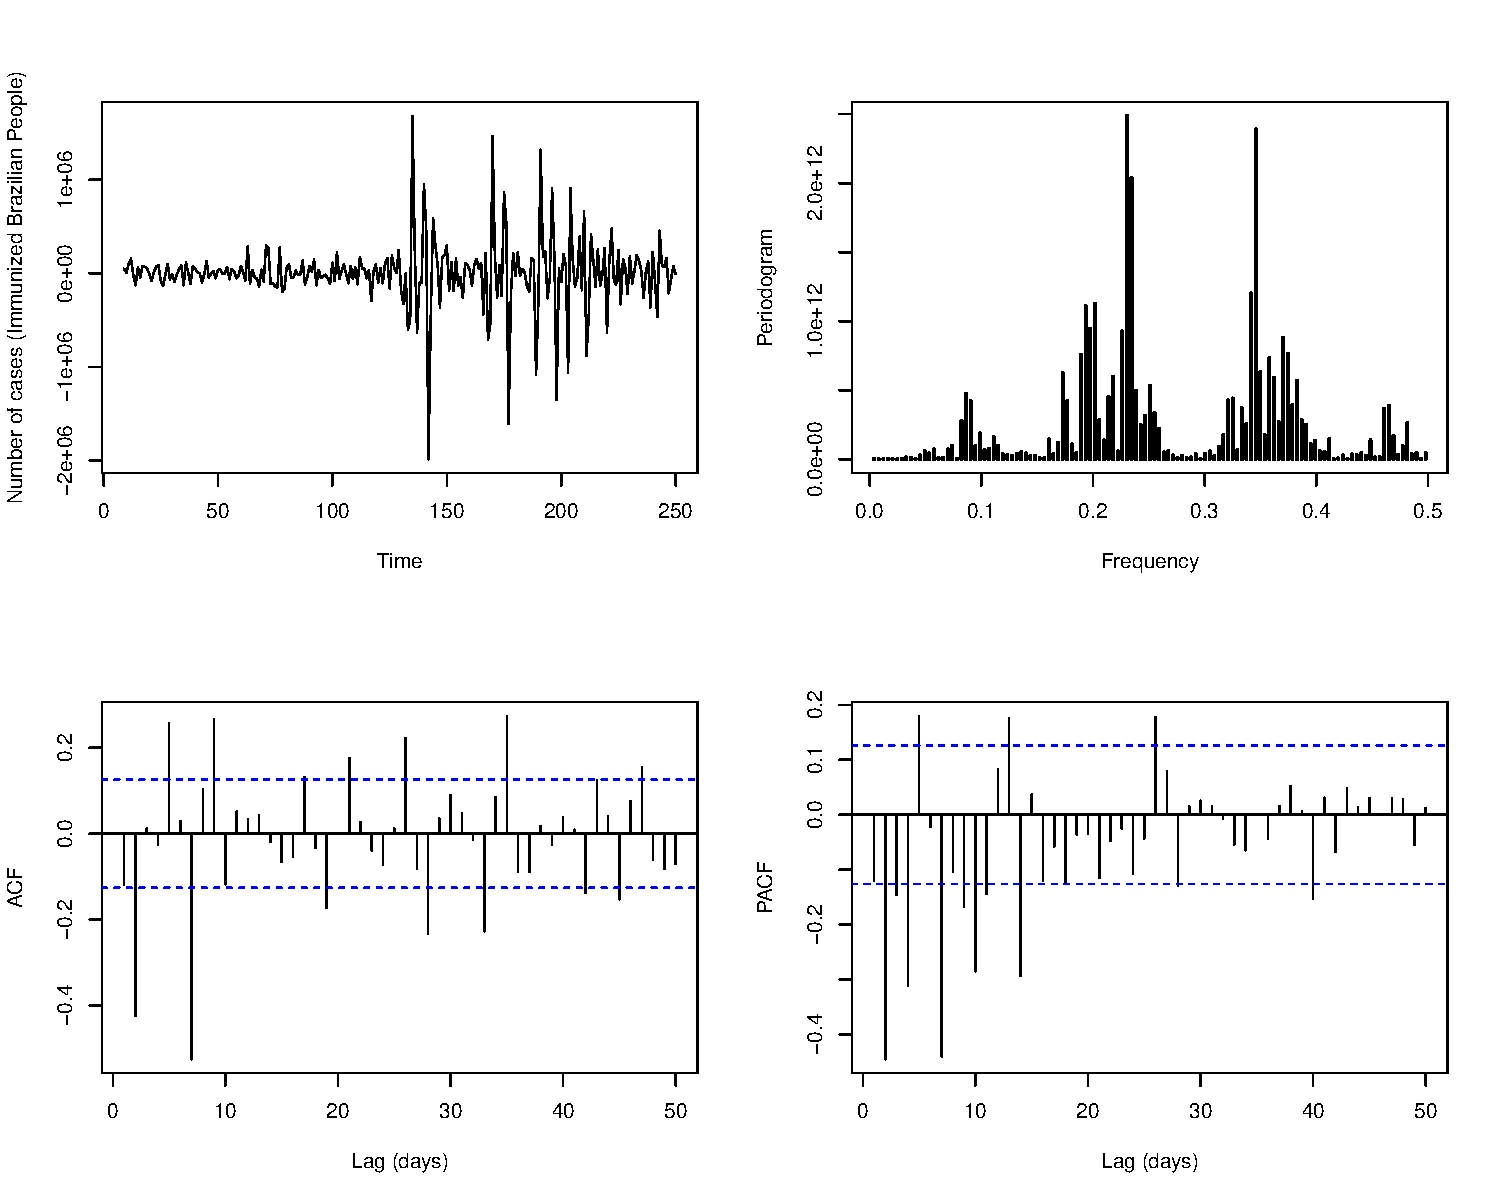
\includegraphics[width=\linewidth]{IF_results_ENG_files/figure-latex/unnamed-chunk-26-1} \end{center}

\textbf{Figure 21}: basic graphs in the analysis of time series applied
to the series of immunized brazilian population considering seasonal
differentiation of seven.

Applying the transformation to the data.

\begin{Shaded}
\begin{Highlighting}[]
\NormalTok{immunizedBR\_log }\OtherTok{\textless{}{-}}
  \FunctionTok{log}\NormalTok{(}\FunctionTok{ts}\NormalTok{(series}\SpecialCharTok{$}\NormalTok{immunized.BR[start\_vac}\SpecialCharTok{:}\NormalTok{end\_vac]))}
\NormalTok{immunizedBR\_dif1 }\OtherTok{\textless{}{-}} \FunctionTok{diff}\NormalTok{(immunizedBR\_log)}
\NormalTok{immunizedBR\_dif7 }\OtherTok{\textless{}{-}} \FunctionTok{diff}\NormalTok{(immunizedBR\_dif1, }\DecValTok{7}\NormalTok{)}

\FunctionTok{par}\NormalTok{(}\AttributeTok{mfrow=}\FunctionTok{c}\NormalTok{(}\DecValTok{2}\NormalTok{,}\DecValTok{2}\NormalTok{))}
\FunctionTok{plot.ts}\NormalTok{(immunizedBR\_dif7,}
        \AttributeTok{xlab =} \StringTok{"Time"}\NormalTok{,}
        \AttributeTok{ylab =} \StringTok{"Number of cases (Immunized Brazilian People)"}\NormalTok{)}
\NormalTok{TSA}\SpecialCharTok{::}\FunctionTok{periodogram}\NormalTok{(immunizedBR\_dif7,}
                 \AttributeTok{xlab =} \StringTok{"Frequency"}\NormalTok{,}
                 \AttributeTok{ylab =} \StringTok{"Periodogram"}\NormalTok{)}
\FunctionTok{acf}\NormalTok{(immunizedBR\_dif7,}
    \AttributeTok{xlab =} \StringTok{"Lag (days)"}\NormalTok{,}
    \AttributeTok{ylab =} \StringTok{"ACF"}\NormalTok{,}
    \AttributeTok{main =} \StringTok{""}\NormalTok{,}
    \AttributeTok{lag.max =} \DecValTok{10}\NormalTok{,}
    \AttributeTok{xaxt =} \StringTok{"n"}\NormalTok{)}
\FunctionTok{axis}\NormalTok{(}\DecValTok{1}\NormalTok{, }\AttributeTok{at =} \DecValTok{1}\SpecialCharTok{:}\DecValTok{10}\NormalTok{)}
\FunctionTok{pacf}\NormalTok{(immunizedBR\_dif7,}
     \AttributeTok{xlab =} \StringTok{"Lag (days)"}\NormalTok{,}
     \AttributeTok{ylab =} \StringTok{"PACF"}\NormalTok{,}
     \AttributeTok{main =} \StringTok{""}\NormalTok{,}
     \AttributeTok{lag.max =} \DecValTok{10}\NormalTok{,}
     \AttributeTok{xaxt =} \StringTok{"n"}\NormalTok{)}
\FunctionTok{axis}\NormalTok{(}\DecValTok{1}\NormalTok{, }\AttributeTok{at =} \DecValTok{1}\SpecialCharTok{:}\DecValTok{10}\NormalTok{)}
\end{Highlighting}
\end{Shaded}

\begin{center}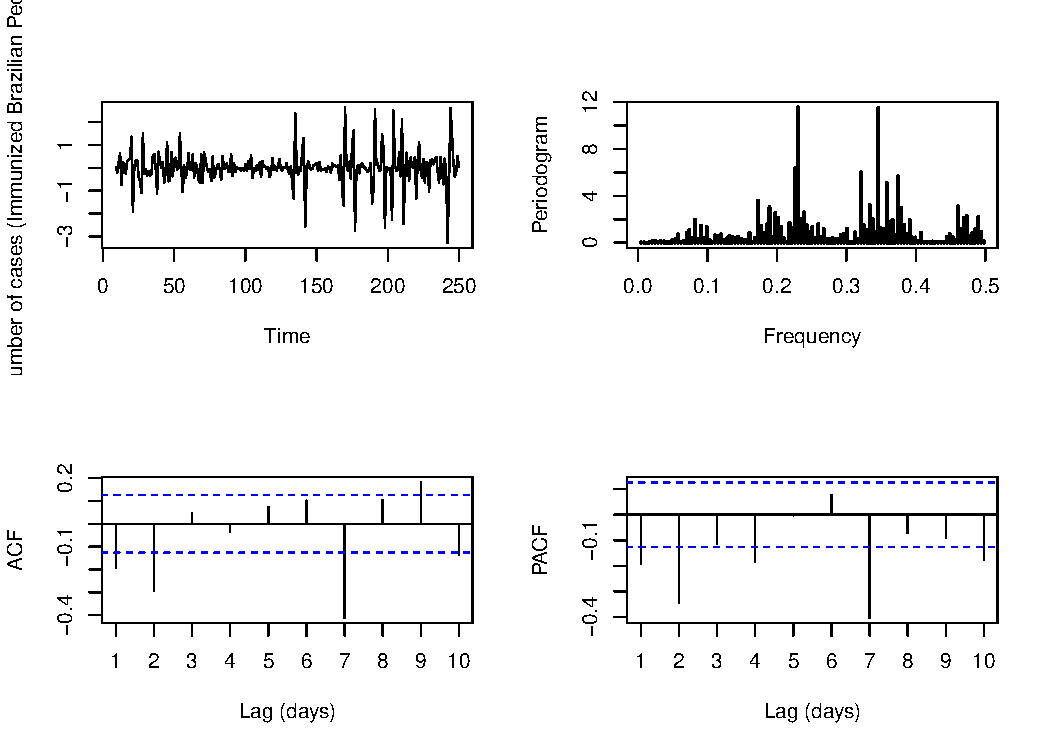
\includegraphics[width=\linewidth]{IF_results_ENG_files/figure-latex/unnamed-chunk-27-1} \end{center}

\textbf{Figure 22}: basic graphs in the analysis of time series applied
to the series of immunized brazilian population considering seasonal
differentiation of seven and logarithmic transformation of the data.

Now, we need to verify if the time series is stationary using the
Augmented Dickey-Fuller Test.

\begin{Shaded}
\begin{Highlighting}[]
\FunctionTok{adf.test}\NormalTok{(immunizedBR\_dif7)}
\end{Highlighting}
\end{Shaded}

\begin{verbatim}
## 
##  Augmented Dickey-Fuller Test
## 
## data:  immunizedBR_dif7
## Dickey-Fuller = -10.484, Lag order = 6, p-value = 0.01
## alternative hypothesis: stationary
\end{verbatim}

The Augmented Dickey-Fuller Test pointed out that the time series is now
stationary.

\section{Totals and daily peaks}

\begin{Shaded}
\begin{Highlighting}[]
\CommentTok{\# ============================================================}
\CommentTok{\# Peaks and totals }
\CommentTok{\# ============================================================}

\NormalTok{period\_start }\OtherTok{\textless{}{-}} \FunctionTok{as.Date}\NormalTok{(}\StringTok{"2021{-}01{-}03"}\NormalTok{)}
\NormalTok{period\_end }\OtherTok{\textless{}{-}} \FunctionTok{as.Date}\NormalTok{(}\StringTok{"2022{-}01{-}01"}\NormalTok{)}

\CommentTok{\# Functions}
\NormalTok{get\_peak }\OtherTok{\textless{}{-}} \ControlFlowTok{function}\NormalTok{(df, value\_col, }\AttributeTok{date\_col =} \StringTok{"date"}\NormalTok{) \{}
\NormalTok{  v }\OtherTok{\textless{}{-}}\NormalTok{ df[[value\_col]]}
\NormalTok{  d }\OtherTok{\textless{}{-}}\NormalTok{ df[[date\_col]]}
\NormalTok{  max\_val }\OtherTok{\textless{}{-}} \FunctionTok{max}\NormalTok{(v)                   }
\NormalTok{  max\_dates }\OtherTok{\textless{}{-}}\NormalTok{ d[v }\SpecialCharTok{==}\NormalTok{ max\_val]}
  \FunctionTok{list}\NormalTok{(}\AttributeTok{max\_value =} \FunctionTok{as.integer}\NormalTok{(max\_val), }\AttributeTok{max\_dates =} \FunctionTok{sort}\NormalTok{(max\_dates))}
\NormalTok{\}}

\NormalTok{fmt\_dates }\OtherTok{\textless{}{-}} \ControlFlowTok{function}\NormalTok{(x) }\FunctionTok{paste}\NormalTok{(}\FunctionTok{format}\NormalTok{(x, }\StringTok{"\%Y{-}\%m{-}\%d"}\NormalTok{), }\AttributeTok{collapse =} \StringTok{"; "}\NormalTok{)}


\CommentTok{\# Totals}
\NormalTok{totals\_tbl }\OtherTok{\textless{}{-}}\NormalTok{ tibble}\SpecialCharTok{::}\FunctionTok{tibble}\NormalTok{(}
  \AttributeTok{indicator =} \FunctionTok{c}\NormalTok{(}
  \StringTok{"Maternal deaths (total in period)"}\NormalTok{,}
  \StringTok{"Partially vaccinated pregnant and postpartum (dose 1, total)"}\NormalTok{,}
  \StringTok{"Fully vaccinated pregnant and postpartum (dose 2+, total)"}\NormalTok{,}
  \StringTok{"Partially vaccinated Brazil (dose 1, total)"}\NormalTok{,}
  \StringTok{"Fully vaccinated Brazil (dose 2+, total)"}
\NormalTok{  ),}
  \AttributeTok{value =} \FunctionTok{c}\NormalTok{(}
  \FunctionTok{sum}\NormalTok{(series}\SpecialCharTok{$}\NormalTok{deaths),}
  \FunctionTok{sum}\NormalTok{(series}\SpecialCharTok{$}\NormalTok{first\_dose.GES),}
  \FunctionTok{sum}\NormalTok{(series}\SpecialCharTok{$}\NormalTok{immunized.GES),}
  \FunctionTok{sum}\NormalTok{(series}\SpecialCharTok{$}\NormalTok{first\_dose.BR),}
  \FunctionTok{sum}\NormalTok{(series}\SpecialCharTok{$}\NormalTok{immunized.BR)}
\NormalTok{  )}
\NormalTok{)}

\CommentTok{\# Peaks}
\NormalTok{pk\_deaths  }\OtherTok{\textless{}{-}} \FunctionTok{get\_peak}\NormalTok{(series, }\StringTok{"deaths"}\NormalTok{,        }\StringTok{"date"}\NormalTok{)}
\NormalTok{pk\_m\_d1    }\OtherTok{\textless{}{-}} \FunctionTok{get\_peak}\NormalTok{(series, }\StringTok{"first\_dose.GES"}\NormalTok{,}\StringTok{"date"}\NormalTok{)}
\NormalTok{pk\_m\_d2    }\OtherTok{\textless{}{-}} \FunctionTok{get\_peak}\NormalTok{(series, }\StringTok{"immunized.GES"}\NormalTok{, }\StringTok{"date"}\NormalTok{)}
\NormalTok{pk\_g\_d1    }\OtherTok{\textless{}{-}} \FunctionTok{get\_peak}\NormalTok{(series, }\StringTok{"first\_dose.BR"}\NormalTok{, }\StringTok{"date"}\NormalTok{)}
\NormalTok{pk\_g\_d2    }\OtherTok{\textless{}{-}} \FunctionTok{get\_peak}\NormalTok{(series, }\StringTok{"immunized.BR"}\NormalTok{,  }\StringTok{"date"}\NormalTok{)}

\NormalTok{peaks\_tbl }\OtherTok{\textless{}{-}}\NormalTok{ tibble}\SpecialCharTok{::}\FunctionTok{tibble}\NormalTok{(}
  \AttributeTok{indicator =} \FunctionTok{c}\NormalTok{(}\StringTok{"Peak of daily maternal deaths"}\NormalTok{,}
  \StringTok{"Peak of daily partially vaccinated pregnant and postpartum"}\NormalTok{,}
  \StringTok{"Peak of daily fully vaccinated pregnant and postpartum"}\NormalTok{,}
  \StringTok{"Peak of daily partially vaccinated Brazil"}\NormalTok{,}
  \StringTok{"Peak of daily fully vaccinated Brazil"}\NormalTok{),}
  \AttributeTok{peak\_value =} \FunctionTok{c}\NormalTok{(pk\_deaths}\SpecialCharTok{$}\NormalTok{max\_value,}
\NormalTok{  pk\_m\_d1}\SpecialCharTok{$}\NormalTok{max\_value,}
\NormalTok{  pk\_m\_d2}\SpecialCharTok{$}\NormalTok{max\_value,}
\NormalTok{  pk\_g\_d1}\SpecialCharTok{$}\NormalTok{max\_value,}
\NormalTok{  pk\_g\_d2}\SpecialCharTok{$}\NormalTok{max\_value),}
  \AttributeTok{peak\_dates =} \FunctionTok{c}\NormalTok{(}\FunctionTok{fmt\_dates}\NormalTok{(pk\_deaths}\SpecialCharTok{$}\NormalTok{max\_dates),}
  \FunctionTok{fmt\_dates}\NormalTok{(pk\_m\_d1}\SpecialCharTok{$}\NormalTok{max\_dates),}
  \FunctionTok{fmt\_dates}\NormalTok{(pk\_m\_d2}\SpecialCharTok{$}\NormalTok{max\_dates),}
  \FunctionTok{fmt\_dates}\NormalTok{(pk\_g\_d1}\SpecialCharTok{$}\NormalTok{max\_dates),}
  \FunctionTok{fmt\_dates}\NormalTok{(pk\_g\_d2}\SpecialCharTok{$}\NormalTok{max\_dates))}
\NormalTok{)}

\CommentTok{\# Tables}
\FunctionTok{cat}\NormalTok{(}\StringTok{"Analysis window: "}\NormalTok{, }\FunctionTok{format}\NormalTok{(period\_start), }\StringTok{" to "}\NormalTok{, }\FunctionTok{format}\NormalTok{(period\_end), }\StringTok{"}\SpecialCharTok{\textbackslash{}n\textbackslash{}n}\StringTok{"}\NormalTok{, }\AttributeTok{sep =} \StringTok{""}\NormalTok{)}
\end{Highlighting}
\end{Shaded}

\begin{verbatim}
## Analysis window: 2021-01-03 to 2022-01-01
\end{verbatim}

\begin{Shaded}
\begin{Highlighting}[]
\FunctionTok{cat}\NormalTok{(}\StringTok{"\#\#\# Totals in the period}\SpecialCharTok{\textbackslash{}n}\StringTok{"}\NormalTok{)}
\end{Highlighting}
\end{Shaded}

\begin{verbatim}
## ### Totals in the period
\end{verbatim}

\begin{Shaded}
\begin{Highlighting}[]
\FunctionTok{kable}\NormalTok{(totals\_tbl, }\AttributeTok{align =} \FunctionTok{c}\NormalTok{(}\StringTok{"l"}\NormalTok{,}\StringTok{"r"}\NormalTok{), }\AttributeTok{format =} \StringTok{"markdown"}\NormalTok{)}
\end{Highlighting}
\end{Shaded}

\begin{longtable}[]{@{}
  >{\raggedright\arraybackslash}p{(\linewidth - 2\tabcolsep) * \real{0.8592}}
  >{\raggedleft\arraybackslash}p{(\linewidth - 2\tabcolsep) * \real{0.1408}}@{}}
\toprule\noalign{}
\begin{minipage}[b]{\linewidth}\raggedright
indicator
\end{minipage} & \begin{minipage}[b]{\linewidth}\raggedleft
value
\end{minipage} \\
\midrule\noalign{}
\endhead
\bottomrule\noalign{}
\endlastfoot
Maternal deaths (total in period) & 1510 \\
Partially vaccinated pregnant and postpartum (dose 1, total) &
1016350 \\
Fully vaccinated pregnant and postpartum (dose 2+, total) & 892231 \\
Partially vaccinated Brazil (dose 1, total) & 157888063 \\
Fully vaccinated Brazil (dose 2+, total) & 160366583 \\
\end{longtable}

\begin{Shaded}
\begin{Highlighting}[]
\FunctionTok{cat}\NormalTok{(}\StringTok{"}\SpecialCharTok{\textbackslash{}n\textbackslash{}n}\StringTok{\#\#\# Daily peaks (value and date[s])}\SpecialCharTok{\textbackslash{}n}\StringTok{"}\NormalTok{)}
\end{Highlighting}
\end{Shaded}

\begin{verbatim}
## 
## 
## ### Daily peaks (value and date[s])
\end{verbatim}

\begin{Shaded}
\begin{Highlighting}[]
\FunctionTok{kable}\NormalTok{(peaks\_tbl, }\AttributeTok{align =} \FunctionTok{c}\NormalTok{(}\StringTok{"l"}\NormalTok{,}\StringTok{"r"}\NormalTok{,}\StringTok{"l"}\NormalTok{), }\AttributeTok{format =} \StringTok{"markdown"}\NormalTok{)}
\end{Highlighting}
\end{Shaded}

\begin{longtable}[]{@{}
  >{\raggedright\arraybackslash}p{(\linewidth - 4\tabcolsep) * \real{0.7284}}
  >{\raggedleft\arraybackslash}p{(\linewidth - 4\tabcolsep) * \real{0.1358}}
  >{\raggedright\arraybackslash}p{(\linewidth - 4\tabcolsep) * \real{0.1358}}@{}}
\toprule\noalign{}
\begin{minipage}[b]{\linewidth}\raggedright
indicator
\end{minipage} & \begin{minipage}[b]{\linewidth}\raggedleft
peak\_value
\end{minipage} & \begin{minipage}[b]{\linewidth}\raggedright
peak\_dates
\end{minipage} \\
\midrule\noalign{}
\endhead
\bottomrule\noalign{}
\endlastfoot
Peak of daily maternal deaths & 24 & 2021-03-18 \\
Peak of daily partially vaccinated pregnant and postpartum & 31148 &
2021-06-22 \\
Peak of daily fully vaccinated pregnant and postpartum & 19552 &
2021-09-09 \\
Peak of daily partially vaccinated Brazil & 1679532 & 2021-08-10 \\
Peak of daily fully vaccinated Brazil & 2301790 & 2021-09-09 \\
\end{longtable}

\section{Impact of COVID-19 vaccination on maternal deaths}

Let's take a look again at our time series, and as we have seen, we are
considering the period after the vaccination of pregnant and postpartum
women did actually start.

\begin{Shaded}
\begin{Highlighting}[]
\CommentTok{\# Set english enviroment}
\FunctionTok{Sys.setlocale}\NormalTok{(}\StringTok{"LC\_TIME"}\NormalTok{, }\StringTok{"English"}\NormalTok{)}
\end{Highlighting}
\end{Shaded}

\begin{verbatim}
## [1] "English_United States.1252"
\end{verbatim}

\begin{Shaded}
\begin{Highlighting}[]
\NormalTok{p1 }\OtherTok{\textless{}{-}} \FunctionTok{ggplot}\NormalTok{(series, }
             \FunctionTok{aes}\NormalTok{(}\AttributeTok{x =}\NormalTok{ date, }\AttributeTok{y =}\NormalTok{ deaths)) }\SpecialCharTok{+} 
  \FunctionTok{geom\_line}\NormalTok{(}\AttributeTok{color =} \StringTok{"red"}\NormalTok{) }\SpecialCharTok{+} 
  \FunctionTok{theme\_bw}\NormalTok{() }\SpecialCharTok{+} 
  \FunctionTok{scale\_x\_date}\NormalTok{(}\AttributeTok{breaks =} \FunctionTok{seq}\NormalTok{(}\FunctionTok{min}\NormalTok{(series}\SpecialCharTok{$}\NormalTok{date),}
                            \FunctionTok{max}\NormalTok{(series}\SpecialCharTok{$}\NormalTok{date), }
                            \AttributeTok{length =} \DecValTok{24}\NormalTok{),}
               \AttributeTok{date\_labels =} \StringTok{"\%b \%d"}\NormalTok{) }\SpecialCharTok{+}
  \FunctionTok{labs}\NormalTok{(}\AttributeTok{x =} \StringTok{"}\SpecialCharTok{\textbackslash{}n}\StringTok{Date"}\NormalTok{, }
       \AttributeTok{y =} \StringTok{"Frequency}\SpecialCharTok{\textbackslash{}n}\StringTok{"}\NormalTok{, }
       \AttributeTok{title =} \StringTok{"Deaths"}\NormalTok{) }\SpecialCharTok{+}
  \FunctionTok{theme}\NormalTok{(}\AttributeTok{axis.text.x =} \FunctionTok{element\_text}\NormalTok{(}\AttributeTok{angle =} \DecValTok{50}\NormalTok{,}
                                   \AttributeTok{hjust =} \DecValTok{1}\NormalTok{),}
        \AttributeTok{panel.background =} \FunctionTok{element\_rect}\NormalTok{(}\AttributeTok{fill =} \StringTok{"white"}\NormalTok{, }\AttributeTok{colour =} \ConstantTok{NA}\NormalTok{),}
        \AttributeTok{panel.border     =} \FunctionTok{element\_rect}\NormalTok{(}\AttributeTok{fill =} \ConstantTok{NA}\NormalTok{, }
                                        \AttributeTok{colour =} \StringTok{"black"}\NormalTok{, }
                                        \AttributeTok{linewidth =} \FloatTok{0.5}\NormalTok{),}
        \AttributeTok{panel.grid.major =} \FunctionTok{element\_blank}\NormalTok{(),}
        \AttributeTok{panel.grid.minor =} \FunctionTok{element\_blank}\NormalTok{(),}
        \AttributeTok{plot.title =} \FunctionTok{element\_text}\NormalTok{(}\AttributeTok{hjust =} \FloatTok{0.5}\NormalTok{,}
                                  \AttributeTok{size =} \DecValTok{12}\NormalTok{,}
                                  \AttributeTok{face =} \StringTok{"bold"}\NormalTok{))}

\NormalTok{p2 }\OtherTok{\textless{}{-}} \FunctionTok{ggplot}\NormalTok{(series, }
             \FunctionTok{aes}\NormalTok{(}\AttributeTok{x =}\NormalTok{ date, }\AttributeTok{y =}\NormalTok{ first\_dose.GES)) }\SpecialCharTok{+} 
  \FunctionTok{geom\_line}\NormalTok{(}\AttributeTok{color =} \StringTok{"steelblue"}\NormalTok{) }\SpecialCharTok{+} 
  \FunctionTok{theme\_bw}\NormalTok{() }\SpecialCharTok{+} 
  \FunctionTok{scale\_x\_date}\NormalTok{(}\AttributeTok{breaks =} \FunctionTok{seq}\NormalTok{(}\FunctionTok{min}\NormalTok{(series}\SpecialCharTok{$}\NormalTok{date),}
                            \FunctionTok{max}\NormalTok{(series}\SpecialCharTok{$}\NormalTok{date), }
                            \AttributeTok{length =} \DecValTok{24}\NormalTok{),}
               \AttributeTok{date\_labels =} \StringTok{"\%b \%d"}\NormalTok{) }\SpecialCharTok{+}
  \FunctionTok{labs}\NormalTok{(}\AttributeTok{x =} \StringTok{"}\SpecialCharTok{\textbackslash{}n}\StringTok{Date"}\NormalTok{, }
       \AttributeTok{y =} \StringTok{"Frequency}\SpecialCharTok{\textbackslash{}n}\StringTok{"}\NormalTok{, }
       \AttributeTok{title =} \StringTok{"Partially vaccinated pregnant and postpartum"}\NormalTok{) }\SpecialCharTok{+}
  \FunctionTok{theme}\NormalTok{(}\AttributeTok{axis.text.x =} \FunctionTok{element\_text}\NormalTok{(}\AttributeTok{angle =} \DecValTok{50}\NormalTok{,}
                                   \AttributeTok{hjust =} \DecValTok{1}\NormalTok{),}
        \AttributeTok{panel.background =} \FunctionTok{element\_rect}\NormalTok{(}\AttributeTok{fill =} \StringTok{"white"}\NormalTok{, }\AttributeTok{colour =} \ConstantTok{NA}\NormalTok{),}
        \AttributeTok{panel.border     =} \FunctionTok{element\_rect}\NormalTok{(}\AttributeTok{fill =} \ConstantTok{NA}\NormalTok{, }
                                        \AttributeTok{colour =} \StringTok{"black"}\NormalTok{, }
                                        \AttributeTok{linewidth =} \FloatTok{0.5}\NormalTok{),}
        \AttributeTok{panel.grid.major =} \FunctionTok{element\_blank}\NormalTok{(),}
        \AttributeTok{panel.grid.minor =} \FunctionTok{element\_blank}\NormalTok{(),}
        \AttributeTok{plot.title =} \FunctionTok{element\_text}\NormalTok{(}\AttributeTok{hjust =} \FloatTok{0.5}\NormalTok{,}
                                  \AttributeTok{size =} \DecValTok{12}\NormalTok{,}
                                  \AttributeTok{face =} \StringTok{"bold"}\NormalTok{))}

\NormalTok{p3 }\OtherTok{\textless{}{-}} \FunctionTok{ggplot}\NormalTok{(series, }
             \FunctionTok{aes}\NormalTok{(}\AttributeTok{x =}\NormalTok{ date, }\AttributeTok{y =}\NormalTok{ first\_dose.BR)) }\SpecialCharTok{+} 
  \FunctionTok{geom\_line}\NormalTok{(}\AttributeTok{color =} \StringTok{"steelblue"}\NormalTok{) }\SpecialCharTok{+} 
  \FunctionTok{theme\_bw}\NormalTok{() }\SpecialCharTok{+} 
  \FunctionTok{scale\_x\_date}\NormalTok{(}\AttributeTok{breaks =} \FunctionTok{seq}\NormalTok{(}\FunctionTok{min}\NormalTok{(series}\SpecialCharTok{$}\NormalTok{date),}
                            \FunctionTok{max}\NormalTok{(series}\SpecialCharTok{$}\NormalTok{date), }
                            \AttributeTok{length =} \DecValTok{24}\NormalTok{),}
               \AttributeTok{date\_labels =} \StringTok{"\%b \%d"}\NormalTok{) }\SpecialCharTok{+}
  \FunctionTok{labs}\NormalTok{(}\AttributeTok{x =} \StringTok{"}\SpecialCharTok{\textbackslash{}n}\StringTok{Date"}\NormalTok{, }
       \AttributeTok{y =} \StringTok{"Frequency}\SpecialCharTok{\textbackslash{}n}\StringTok{"}\NormalTok{, }
       \AttributeTok{title =} \StringTok{"Partially vaccinated Brazil"}\NormalTok{) }\SpecialCharTok{+}
  \FunctionTok{theme}\NormalTok{(}\AttributeTok{axis.text.x =} \FunctionTok{element\_text}\NormalTok{(}\AttributeTok{angle =} \DecValTok{50}\NormalTok{,}
                                   \AttributeTok{hjust =} \DecValTok{1}\NormalTok{),}
        \AttributeTok{panel.background =} \FunctionTok{element\_rect}\NormalTok{(}\AttributeTok{fill =} \StringTok{"white"}\NormalTok{, }\AttributeTok{colour =} \ConstantTok{NA}\NormalTok{),}
        \AttributeTok{panel.border     =} \FunctionTok{element\_rect}\NormalTok{(}\AttributeTok{fill =} \ConstantTok{NA}\NormalTok{, }
                                        \AttributeTok{colour =} \StringTok{"black"}\NormalTok{, }
                                        \AttributeTok{linewidth =} \FloatTok{0.5}\NormalTok{),}
        \AttributeTok{panel.grid.major =} \FunctionTok{element\_blank}\NormalTok{(),}
        \AttributeTok{panel.grid.minor =} \FunctionTok{element\_blank}\NormalTok{(),}
        \AttributeTok{plot.title =} \FunctionTok{element\_text}\NormalTok{(}\AttributeTok{hjust =} \FloatTok{0.5}\NormalTok{,}
                                  \AttributeTok{size =} \DecValTok{12}\NormalTok{,}
                                  \AttributeTok{face =} \StringTok{"bold"}\NormalTok{))}

\NormalTok{p4 }\OtherTok{\textless{}{-}} \FunctionTok{ggplot}\NormalTok{(series, }
             \FunctionTok{aes}\NormalTok{(}\AttributeTok{x =}\NormalTok{ date, }\AttributeTok{y =}\NormalTok{ immunized.GES)) }\SpecialCharTok{+} 
  \FunctionTok{geom\_line}\NormalTok{(}\AttributeTok{color =} \StringTok{"steelblue"}\NormalTok{) }\SpecialCharTok{+} 
  \FunctionTok{theme\_bw}\NormalTok{() }\SpecialCharTok{+} 
  \FunctionTok{scale\_x\_date}\NormalTok{(}\AttributeTok{breaks =} \FunctionTok{seq}\NormalTok{(}\FunctionTok{min}\NormalTok{(series}\SpecialCharTok{$}\NormalTok{date),}
                            \FunctionTok{max}\NormalTok{(series}\SpecialCharTok{$}\NormalTok{date), }
                            \AttributeTok{length =} \DecValTok{24}\NormalTok{),}
               \AttributeTok{date\_labels =} \StringTok{"\%b \%d"}\NormalTok{) }\SpecialCharTok{+}
  \FunctionTok{labs}\NormalTok{(}\AttributeTok{x =} \StringTok{"}\SpecialCharTok{\textbackslash{}n}\StringTok{Date"}\NormalTok{, }
       \AttributeTok{y =} \StringTok{"Frequency}\SpecialCharTok{\textbackslash{}n}\StringTok{"}\NormalTok{, }
       \AttributeTok{title =} \StringTok{"Fully vaccinated pregnant and postpartum"}\NormalTok{) }\SpecialCharTok{+}
  \FunctionTok{theme}\NormalTok{(}\AttributeTok{axis.text.x =} \FunctionTok{element\_text}\NormalTok{(}\AttributeTok{angle =} \DecValTok{50}\NormalTok{,}
                                   \AttributeTok{hjust =} \DecValTok{1}\NormalTok{),}
        \AttributeTok{panel.background =} \FunctionTok{element\_rect}\NormalTok{(}\AttributeTok{fill =} \StringTok{"white"}\NormalTok{, }\AttributeTok{colour =} \ConstantTok{NA}\NormalTok{),}
        \AttributeTok{panel.border     =} \FunctionTok{element\_rect}\NormalTok{(}\AttributeTok{fill =} \ConstantTok{NA}\NormalTok{, }
                                        \AttributeTok{colour =} \StringTok{"black"}\NormalTok{, }
                                        \AttributeTok{linewidth =} \FloatTok{0.5}\NormalTok{),}
        \AttributeTok{panel.grid.major =} \FunctionTok{element\_blank}\NormalTok{(),}
        \AttributeTok{panel.grid.minor =} \FunctionTok{element\_blank}\NormalTok{(),}
        \AttributeTok{plot.title =} \FunctionTok{element\_text}\NormalTok{(}\AttributeTok{hjust =} \FloatTok{0.5}\NormalTok{,}
                                  \AttributeTok{size =} \DecValTok{12}\NormalTok{,}
                                  \AttributeTok{face =} \StringTok{"bold"}\NormalTok{))}

\NormalTok{p5 }\OtherTok{\textless{}{-}} \FunctionTok{ggplot}\NormalTok{(series, }
             \FunctionTok{aes}\NormalTok{(}\AttributeTok{x =}\NormalTok{ date, }\AttributeTok{y =}\NormalTok{ immunized.BR)) }\SpecialCharTok{+} 
  \FunctionTok{geom\_line}\NormalTok{(}\AttributeTok{color =} \StringTok{"steelblue"}\NormalTok{) }\SpecialCharTok{+} 
  \FunctionTok{theme\_bw}\NormalTok{() }\SpecialCharTok{+} 
  \FunctionTok{scale\_x\_date}\NormalTok{(}\AttributeTok{breaks =} \FunctionTok{seq}\NormalTok{(}\FunctionTok{min}\NormalTok{(series}\SpecialCharTok{$}\NormalTok{date),}
                            \FunctionTok{max}\NormalTok{(series}\SpecialCharTok{$}\NormalTok{date), }
                            \AttributeTok{length =} \DecValTok{24}\NormalTok{),}
               \AttributeTok{date\_labels =} \StringTok{"\%b \%d"}\NormalTok{) }\SpecialCharTok{+}
  \FunctionTok{labs}\NormalTok{(}\AttributeTok{x =} \StringTok{"}\SpecialCharTok{\textbackslash{}n}\StringTok{Date"}\NormalTok{, }
       \AttributeTok{y =} \StringTok{"Frequency}\SpecialCharTok{\textbackslash{}n}\StringTok{"}\NormalTok{, }
       \AttributeTok{title =} \StringTok{"Fully vaccinated Brazil"}\NormalTok{) }\SpecialCharTok{+}
  \FunctionTok{theme}\NormalTok{(}\AttributeTok{axis.text.x =} \FunctionTok{element\_text}\NormalTok{(}\AttributeTok{angle =} \DecValTok{50}\NormalTok{,}
                                   \AttributeTok{hjust =} \DecValTok{1}\NormalTok{),}
        \AttributeTok{panel.background =} \FunctionTok{element\_rect}\NormalTok{(}\AttributeTok{fill =} \StringTok{"white"}\NormalTok{, }\AttributeTok{colour =} \ConstantTok{NA}\NormalTok{),}
        \AttributeTok{panel.border     =} \FunctionTok{element\_rect}\NormalTok{(}\AttributeTok{fill =} \ConstantTok{NA}\NormalTok{, }
                                        \AttributeTok{colour =} \StringTok{"black"}\NormalTok{, }
                                        \AttributeTok{linewidth =} \FloatTok{0.5}\NormalTok{),}
        \AttributeTok{panel.grid.major =} \FunctionTok{element\_blank}\NormalTok{(),}
        \AttributeTok{panel.grid.minor =} \FunctionTok{element\_blank}\NormalTok{(),}
        \AttributeTok{plot.title =} \FunctionTok{element\_text}\NormalTok{(}\AttributeTok{hjust =} \FloatTok{0.5}\NormalTok{,}
                                  \AttributeTok{size =} \DecValTok{12}\NormalTok{,}
                                  \AttributeTok{face =} \StringTok{"bold"}\NormalTok{))}

\NormalTok{design }\OtherTok{\textless{}{-}} \StringTok{"}
\StringTok{  12}
\StringTok{  34}
\StringTok{  5\#}
\StringTok{"}

\NormalTok{p1 }\SpecialCharTok{+}\NormalTok{ p2 }\SpecialCharTok{+}\NormalTok{ p3 }\SpecialCharTok{+}\NormalTok{ p4 }\SpecialCharTok{+}\NormalTok{ p5 }\SpecialCharTok{+} \FunctionTok{plot\_layout}\NormalTok{(}\AttributeTok{design =}\NormalTok{ design)}
\end{Highlighting}
\end{Shaded}

\begin{center}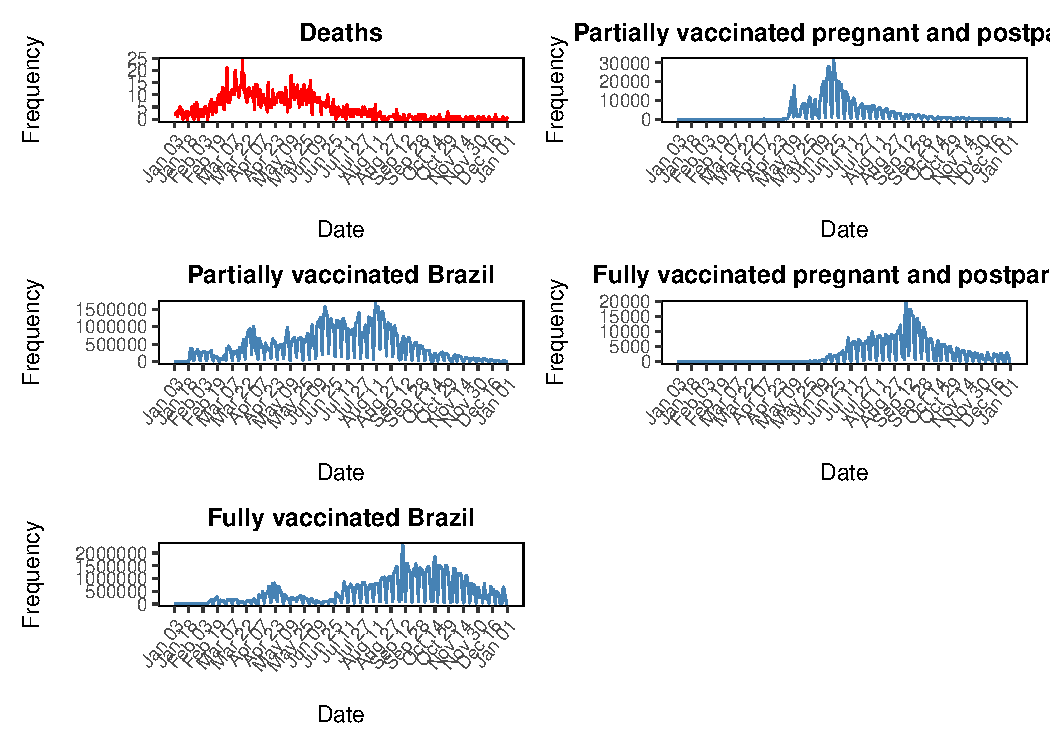
\includegraphics[width=\linewidth]{IF_results_ENG_files/figure-latex/unnamed-chunk-31-1} \end{center}

\textbf{Figure 23A}: graphs of all time series.

\begin{Shaded}
\begin{Highlighting}[]
\NormalTok{p1 }\OtherTok{\textless{}{-}} \FunctionTok{ggplot}\NormalTok{(series[start\_vac}\SpecialCharTok{:}\NormalTok{end\_vac,], }
             \FunctionTok{aes}\NormalTok{(}\AttributeTok{x =}\NormalTok{ date, }\AttributeTok{y =}\NormalTok{ deaths)) }\SpecialCharTok{+} 
  \FunctionTok{geom\_line}\NormalTok{(}\AttributeTok{color =} \StringTok{"red"}\NormalTok{) }\SpecialCharTok{+} 
  \FunctionTok{theme\_bw}\NormalTok{() }\SpecialCharTok{+} 
  \FunctionTok{scale\_x\_date}\NormalTok{(}\AttributeTok{breaks =} \FunctionTok{seq}\NormalTok{(}\FunctionTok{min}\NormalTok{(series[start\_vac}\SpecialCharTok{:}\NormalTok{end\_vac,]}\SpecialCharTok{$}\NormalTok{date),}
                            \FunctionTok{max}\NormalTok{(series[start\_vac}\SpecialCharTok{:}\NormalTok{end\_vac,]}\SpecialCharTok{$}\NormalTok{date), }
                            \AttributeTok{length =} \DecValTok{24}\NormalTok{),}
               \AttributeTok{date\_labels =} \StringTok{"\%b \%d"}\NormalTok{) }\SpecialCharTok{+}
  \FunctionTok{labs}\NormalTok{(}\AttributeTok{x =} \StringTok{"}\SpecialCharTok{\textbackslash{}n}\StringTok{Date"}\NormalTok{, }
       \AttributeTok{y =} \StringTok{"Frequency}\SpecialCharTok{\textbackslash{}n}\StringTok{"}\NormalTok{, }
       \AttributeTok{title =} \StringTok{"Deaths"}\NormalTok{) }\SpecialCharTok{+}
  \FunctionTok{theme}\NormalTok{(}\AttributeTok{axis.text.x =} \FunctionTok{element\_text}\NormalTok{(}\AttributeTok{angle =} \DecValTok{50}\NormalTok{,}
                                   \AttributeTok{hjust =} \DecValTok{1}\NormalTok{),}
        \AttributeTok{panel.background =} \FunctionTok{element\_rect}\NormalTok{(}\AttributeTok{fill =} \StringTok{"white"}\NormalTok{, }\AttributeTok{colour =} \ConstantTok{NA}\NormalTok{),}
        \AttributeTok{panel.border     =} \FunctionTok{element\_rect}\NormalTok{(}\AttributeTok{fill =} \ConstantTok{NA}\NormalTok{, }
                                        \AttributeTok{colour =} \StringTok{"black"}\NormalTok{, }
                                        \AttributeTok{linewidth =} \FloatTok{0.5}\NormalTok{),}
        \AttributeTok{panel.grid.major =} \FunctionTok{element\_blank}\NormalTok{(),}
        \AttributeTok{panel.grid.minor =} \FunctionTok{element\_blank}\NormalTok{(),}
        \AttributeTok{plot.title =} \FunctionTok{element\_text}\NormalTok{(}\AttributeTok{hjust =} \FloatTok{0.5}\NormalTok{,}
                                  \AttributeTok{size =} \DecValTok{12}\NormalTok{,}
                                  \AttributeTok{face =} \StringTok{"bold"}\NormalTok{))}

\NormalTok{p2 }\OtherTok{\textless{}{-}} \FunctionTok{ggplot}\NormalTok{(series[start\_vac}\SpecialCharTok{:}\NormalTok{end\_vac,], }
             \FunctionTok{aes}\NormalTok{(}\AttributeTok{x =}\NormalTok{ date, }\AttributeTok{y =}\NormalTok{ first\_dose.GES)) }\SpecialCharTok{+} 
  \FunctionTok{geom\_line}\NormalTok{(}\AttributeTok{color =} \StringTok{"steelblue"}\NormalTok{) }\SpecialCharTok{+} 
  \FunctionTok{theme\_bw}\NormalTok{() }\SpecialCharTok{+} 
  \FunctionTok{scale\_x\_date}\NormalTok{(}\AttributeTok{breaks =} \FunctionTok{seq}\NormalTok{(}\FunctionTok{min}\NormalTok{(series[start\_vac}\SpecialCharTok{:}\NormalTok{end\_vac,]}\SpecialCharTok{$}\NormalTok{date),}
                            \FunctionTok{max}\NormalTok{(series[start\_vac}\SpecialCharTok{:}\NormalTok{end\_vac,]}\SpecialCharTok{$}\NormalTok{date), }
                            \AttributeTok{length =} \DecValTok{24}\NormalTok{),}
               \AttributeTok{date\_labels =} \StringTok{"\%b \%d"}\NormalTok{) }\SpecialCharTok{+}
  \FunctionTok{labs}\NormalTok{(}\AttributeTok{x =} \StringTok{"}\SpecialCharTok{\textbackslash{}n}\StringTok{Date"}\NormalTok{, }
       \AttributeTok{y =} \StringTok{"Frequency}\SpecialCharTok{\textbackslash{}n}\StringTok{"}\NormalTok{, }
       \AttributeTok{title =} \StringTok{"Partially vaccinated pregnant and postpartum"}\NormalTok{) }\SpecialCharTok{+}
  \FunctionTok{theme}\NormalTok{(}\AttributeTok{axis.text.x =} \FunctionTok{element\_text}\NormalTok{(}\AttributeTok{angle =} \DecValTok{50}\NormalTok{,}
                                   \AttributeTok{hjust =} \DecValTok{1}\NormalTok{),}
        \AttributeTok{panel.background =} \FunctionTok{element\_rect}\NormalTok{(}\AttributeTok{fill =} \StringTok{"white"}\NormalTok{, }\AttributeTok{colour =} \ConstantTok{NA}\NormalTok{),}
        \AttributeTok{panel.border     =} \FunctionTok{element\_rect}\NormalTok{(}\AttributeTok{fill =} \ConstantTok{NA}\NormalTok{, }
                                        \AttributeTok{colour =} \StringTok{"black"}\NormalTok{, }
                                        \AttributeTok{linewidth =} \FloatTok{0.5}\NormalTok{),}
        \AttributeTok{panel.grid.major =} \FunctionTok{element\_blank}\NormalTok{(),}
        \AttributeTok{panel.grid.minor =} \FunctionTok{element\_blank}\NormalTok{(),}
        \AttributeTok{plot.title =} \FunctionTok{element\_text}\NormalTok{(}\AttributeTok{hjust =} \FloatTok{0.5}\NormalTok{,}
                                  \AttributeTok{size =} \DecValTok{12}\NormalTok{,}
                                  \AttributeTok{face =} \StringTok{"bold"}\NormalTok{))}

\NormalTok{p3 }\OtherTok{\textless{}{-}} \FunctionTok{ggplot}\NormalTok{(series[start\_vac}\SpecialCharTok{:}\NormalTok{end\_vac,], }
             \FunctionTok{aes}\NormalTok{(}\AttributeTok{x =}\NormalTok{ date, }\AttributeTok{y =}\NormalTok{ first\_dose.BR)) }\SpecialCharTok{+} 
  \FunctionTok{geom\_line}\NormalTok{(}\AttributeTok{color =} \StringTok{"steelblue"}\NormalTok{) }\SpecialCharTok{+} 
  \FunctionTok{theme\_bw}\NormalTok{() }\SpecialCharTok{+} 
  \FunctionTok{scale\_x\_date}\NormalTok{(}\AttributeTok{breaks =} \FunctionTok{seq}\NormalTok{(}\FunctionTok{min}\NormalTok{(series[start\_vac}\SpecialCharTok{:}\NormalTok{end\_vac,]}\SpecialCharTok{$}\NormalTok{date),}
                            \FunctionTok{max}\NormalTok{(series[start\_vac}\SpecialCharTok{:}\NormalTok{end\_vac,]}\SpecialCharTok{$}\NormalTok{date), }
                            \AttributeTok{length =} \DecValTok{24}\NormalTok{),}
               \AttributeTok{date\_labels =} \StringTok{"\%b \%d"}\NormalTok{) }\SpecialCharTok{+}
  \FunctionTok{labs}\NormalTok{(}\AttributeTok{x =} \StringTok{"}\SpecialCharTok{\textbackslash{}n}\StringTok{Date"}\NormalTok{, }
       \AttributeTok{y =} \StringTok{"Frequency}\SpecialCharTok{\textbackslash{}n}\StringTok{"}\NormalTok{, }
       \AttributeTok{title =} \StringTok{"Partially vaccinated Brazil"}\NormalTok{) }\SpecialCharTok{+}
  \FunctionTok{theme}\NormalTok{(}\AttributeTok{axis.text.x =} \FunctionTok{element\_text}\NormalTok{(}\AttributeTok{angle =} \DecValTok{50}\NormalTok{,}
                                   \AttributeTok{hjust =} \DecValTok{1}\NormalTok{),}
        \AttributeTok{panel.background =} \FunctionTok{element\_rect}\NormalTok{(}\AttributeTok{fill =} \StringTok{"white"}\NormalTok{, }\AttributeTok{colour =} \ConstantTok{NA}\NormalTok{),}
        \AttributeTok{panel.border     =} \FunctionTok{element\_rect}\NormalTok{(}\AttributeTok{fill =} \ConstantTok{NA}\NormalTok{, }
                                        \AttributeTok{colour =} \StringTok{"black"}\NormalTok{, }
                                        \AttributeTok{linewidth =} \FloatTok{0.5}\NormalTok{),}
        \AttributeTok{panel.grid.major =} \FunctionTok{element\_blank}\NormalTok{(),}
        \AttributeTok{panel.grid.minor =} \FunctionTok{element\_blank}\NormalTok{(),}
        \AttributeTok{plot.title =} \FunctionTok{element\_text}\NormalTok{(}\AttributeTok{hjust =} \FloatTok{0.5}\NormalTok{,}
                                  \AttributeTok{size =} \DecValTok{12}\NormalTok{,}
                                  \AttributeTok{face =} \StringTok{"bold"}\NormalTok{))}

\NormalTok{p4 }\OtherTok{\textless{}{-}} \FunctionTok{ggplot}\NormalTok{(series[start\_vac}\SpecialCharTok{:}\NormalTok{end\_vac,], }
             \FunctionTok{aes}\NormalTok{(}\AttributeTok{x =}\NormalTok{ date, }\AttributeTok{y =}\NormalTok{ immunized.GES)) }\SpecialCharTok{+} 
  \FunctionTok{geom\_line}\NormalTok{(}\AttributeTok{color =} \StringTok{"steelblue"}\NormalTok{) }\SpecialCharTok{+} 
  \FunctionTok{theme\_bw}\NormalTok{() }\SpecialCharTok{+} 
  \FunctionTok{scale\_x\_date}\NormalTok{(}\AttributeTok{breaks =} \FunctionTok{seq}\NormalTok{(}\FunctionTok{min}\NormalTok{(series[start\_vac}\SpecialCharTok{:}\NormalTok{end\_vac,]}\SpecialCharTok{$}\NormalTok{date),}
                            \FunctionTok{max}\NormalTok{(series[start\_vac}\SpecialCharTok{:}\NormalTok{end\_vac,]}\SpecialCharTok{$}\NormalTok{date), }
                            \AttributeTok{length =} \DecValTok{24}\NormalTok{),}
               \AttributeTok{date\_labels =} \StringTok{"\%b \%d"}\NormalTok{) }\SpecialCharTok{+}
  \FunctionTok{labs}\NormalTok{(}\AttributeTok{x =} \StringTok{"}\SpecialCharTok{\textbackslash{}n}\StringTok{Date"}\NormalTok{, }
       \AttributeTok{y =} \StringTok{"Frequency}\SpecialCharTok{\textbackslash{}n}\StringTok{"}\NormalTok{, }
       \AttributeTok{title =} \StringTok{"Fully vaccinated pregnant and postpartum"}\NormalTok{) }\SpecialCharTok{+}
  \FunctionTok{theme}\NormalTok{(}\AttributeTok{axis.text.x =} \FunctionTok{element\_text}\NormalTok{(}\AttributeTok{angle =} \DecValTok{50}\NormalTok{,}
                                   \AttributeTok{hjust =} \DecValTok{1}\NormalTok{),}
        \AttributeTok{panel.background =} \FunctionTok{element\_rect}\NormalTok{(}\AttributeTok{fill =} \StringTok{"white"}\NormalTok{, }\AttributeTok{colour =} \ConstantTok{NA}\NormalTok{),}
        \AttributeTok{panel.border     =} \FunctionTok{element\_rect}\NormalTok{(}\AttributeTok{fill =} \ConstantTok{NA}\NormalTok{, }
                                        \AttributeTok{colour =} \StringTok{"black"}\NormalTok{, }
                                        \AttributeTok{linewidth =} \FloatTok{0.5}\NormalTok{),}
        \AttributeTok{panel.grid.major =} \FunctionTok{element\_blank}\NormalTok{(),}
        \AttributeTok{panel.grid.minor =} \FunctionTok{element\_blank}\NormalTok{(),}
        \AttributeTok{plot.title =} \FunctionTok{element\_text}\NormalTok{(}\AttributeTok{hjust =} \FloatTok{0.5}\NormalTok{,}
                                  \AttributeTok{size =} \DecValTok{12}\NormalTok{,}
                                  \AttributeTok{face =} \StringTok{"bold"}\NormalTok{))}

\NormalTok{p5 }\OtherTok{\textless{}{-}} \FunctionTok{ggplot}\NormalTok{(series[start\_vac}\SpecialCharTok{:}\NormalTok{end\_vac,], }
             \FunctionTok{aes}\NormalTok{(}\AttributeTok{x =}\NormalTok{ date, }\AttributeTok{y =}\NormalTok{ immunized.BR)) }\SpecialCharTok{+} 
  \FunctionTok{geom\_line}\NormalTok{(}\AttributeTok{color =} \StringTok{"steelblue"}\NormalTok{) }\SpecialCharTok{+} 
  \FunctionTok{theme\_bw}\NormalTok{() }\SpecialCharTok{+} 
  \FunctionTok{scale\_x\_date}\NormalTok{(}\AttributeTok{breaks =} \FunctionTok{seq}\NormalTok{(}\FunctionTok{min}\NormalTok{(series[start\_vac}\SpecialCharTok{:}\NormalTok{end\_vac,]}\SpecialCharTok{$}\NormalTok{date),}
                            \FunctionTok{max}\NormalTok{(series[start\_vac}\SpecialCharTok{:}\NormalTok{end\_vac,]}\SpecialCharTok{$}\NormalTok{date), }
                            \AttributeTok{length =} \DecValTok{24}\NormalTok{),}
               \AttributeTok{date\_labels =} \StringTok{"\%b \%d"}\NormalTok{) }\SpecialCharTok{+}
  \FunctionTok{labs}\NormalTok{(}\AttributeTok{x =} \StringTok{"}\SpecialCharTok{\textbackslash{}n}\StringTok{Date"}\NormalTok{, }
       \AttributeTok{y =} \StringTok{"Frequency}\SpecialCharTok{\textbackslash{}n}\StringTok{"}\NormalTok{, }
       \AttributeTok{title =} \StringTok{"Fully vaccinated Brazil"}\NormalTok{) }\SpecialCharTok{+}
  \FunctionTok{theme}\NormalTok{(}\AttributeTok{axis.text.x =} \FunctionTok{element\_text}\NormalTok{(}\AttributeTok{angle =} \DecValTok{50}\NormalTok{,}
                                   \AttributeTok{hjust =} \DecValTok{1}\NormalTok{),}
        \AttributeTok{panel.background =} \FunctionTok{element\_rect}\NormalTok{(}\AttributeTok{fill =} \StringTok{"white"}\NormalTok{, }\AttributeTok{colour =} \ConstantTok{NA}\NormalTok{),}
        \AttributeTok{panel.border     =} \FunctionTok{element\_rect}\NormalTok{(}\AttributeTok{fill =} \ConstantTok{NA}\NormalTok{, }
                                        \AttributeTok{colour =} \StringTok{"black"}\NormalTok{, }
                                        \AttributeTok{linewidth =} \FloatTok{0.5}\NormalTok{),}
        \AttributeTok{panel.grid.major =} \FunctionTok{element\_blank}\NormalTok{(),}
        \AttributeTok{panel.grid.minor =} \FunctionTok{element\_blank}\NormalTok{(),}
        \AttributeTok{plot.title =} \FunctionTok{element\_text}\NormalTok{(}\AttributeTok{hjust =} \FloatTok{0.5}\NormalTok{,}
                                  \AttributeTok{size =} \DecValTok{12}\NormalTok{,}
                                  \AttributeTok{face =} \StringTok{"bold"}\NormalTok{))}

\NormalTok{design }\OtherTok{\textless{}{-}} \StringTok{"}
\StringTok{  12}
\StringTok{  34}
\StringTok{  5\#}
\StringTok{"}

\NormalTok{p1 }\SpecialCharTok{+}\NormalTok{ p2 }\SpecialCharTok{+}\NormalTok{ p3 }\SpecialCharTok{+}\NormalTok{ p4 }\SpecialCharTok{+}\NormalTok{ p5 }\SpecialCharTok{+} \FunctionTok{plot\_layout}\NormalTok{(}\AttributeTok{design =}\NormalTok{ design)}
\end{Highlighting}
\end{Shaded}

\begin{center}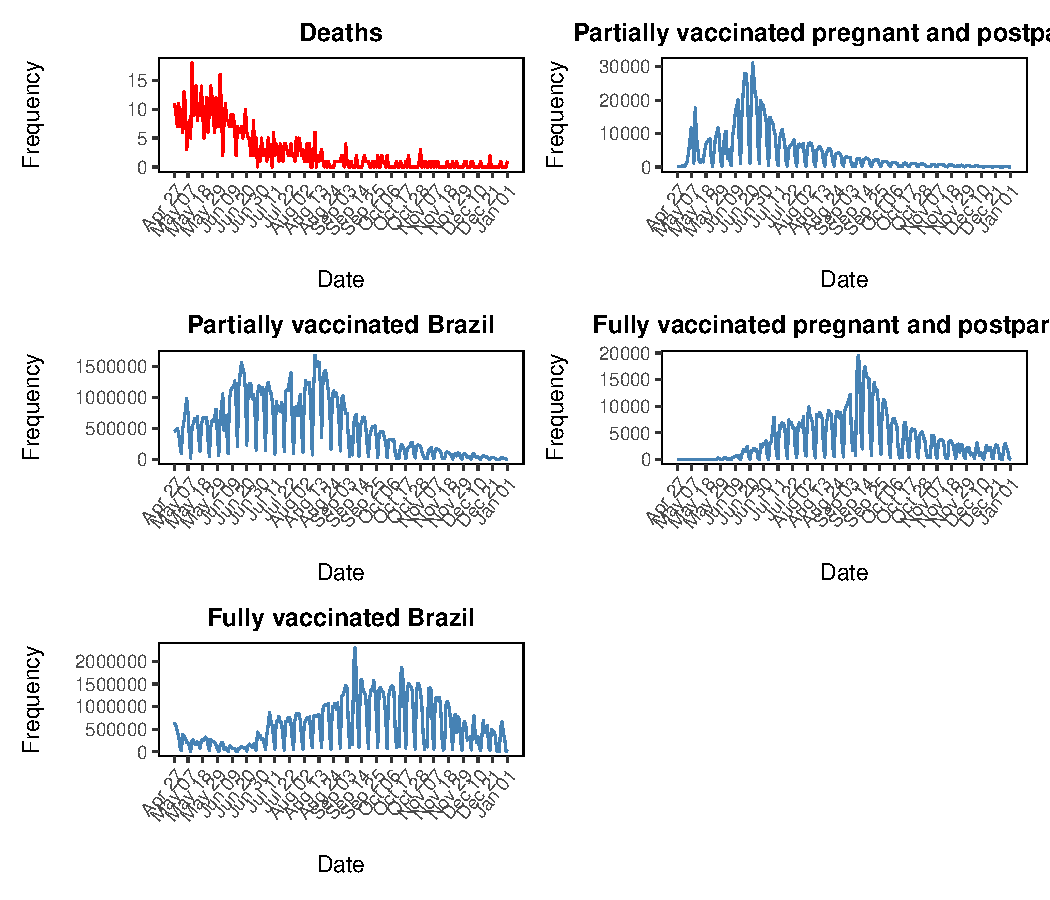
\includegraphics[width=\linewidth]{IF_results_ENG_files/figure-latex/unnamed-chunk-32-1} \end{center}

\textbf{Figure 23B}: graphs of all time series starting on April 27,
2021.

For the following analyses, we need all the time series in Figure 23B to
be stationary. Thus, the entire procedure performed during the
univariate analysis of the series will be considered.

\begin{Shaded}
\begin{Highlighting}[]
\NormalTok{series\_vac }\OtherTok{\textless{}{-}}\NormalTok{ series[start\_vac}\SpecialCharTok{:}\NormalTok{end\_vac,]}
\NormalTok{series\_vac[,}\StringTok{\textquotesingle{}deaths\textquotesingle{}}\NormalTok{] }\OtherTok{\textless{}{-}}\NormalTok{ series\_vac[,}\StringTok{\textquotesingle{}deaths\textquotesingle{}}\NormalTok{] }\SpecialCharTok{+} \FloatTok{3.}
\NormalTok{series\_vac[,}\StringTok{\textquotesingle{}first\_dose.GES\textquotesingle{}}\NormalTok{] }\OtherTok{\textless{}{-}}\NormalTok{ series\_vac[,}\StringTok{\textquotesingle{}first\_dose.GES\textquotesingle{}}\NormalTok{] }\SpecialCharTok{+} \FloatTok{4000.}
\NormalTok{series\_vac[,}\StringTok{\textquotesingle{}immunized.GES\textquotesingle{}}\NormalTok{] }\OtherTok{\textless{}{-}}\NormalTok{ series\_vac[,}\StringTok{\textquotesingle{}immunized.GES\textquotesingle{}}\NormalTok{] }\SpecialCharTok{+} \FloatTok{3500.}

\NormalTok{lseries }\OtherTok{\textless{}{-}} \FunctionTok{log}\NormalTok{(series\_vac[,}\SpecialCharTok{{-}}\DecValTok{1}\NormalTok{])}

\NormalTok{df.diff  }\OtherTok{\textless{}{-}}\NormalTok{  base}\SpecialCharTok{::}\FunctionTok{diff}\NormalTok{(}\FunctionTok{as.matrix}\NormalTok{(lseries), }\AttributeTok{lag =} \DecValTok{1}\NormalTok{)}
\NormalTok{df.diff0  }\OtherTok{\textless{}{-}}\NormalTok{  base}\SpecialCharTok{::}\FunctionTok{diff}\NormalTok{(df.diff[,}\SpecialCharTok{{-}}\DecValTok{1}\NormalTok{],}\AttributeTok{lag =} \DecValTok{7}\NormalTok{)}
\NormalTok{df.diff3 }\OtherTok{\textless{}{-}} \FunctionTok{cbind}\NormalTok{(df.diff[}\DecValTok{8}\SpecialCharTok{:}\DecValTok{249}\NormalTok{,}\DecValTok{1}\NormalTok{], df.diff0)}
\FunctionTok{colnames}\NormalTok{(df.diff3) }\OtherTok{\textless{}{-}} \FunctionTok{c}\NormalTok{(}\StringTok{"deaths"}\NormalTok{,}
                        \StringTok{"first\_dose.BR"}\NormalTok{,}
                        \StringTok{"immunized.BR"}\NormalTok{,}
                        \StringTok{"first\_dose.GES"}\NormalTok{,}
                        \StringTok{"immunized.GES"}\NormalTok{)}
\end{Highlighting}
\end{Shaded}

The analysis of the impact between the vaccination series and the series
of deaths of pregnant and postpartum women will be performed using
impulse response functions(IRF). This analysis consists of using
vaccination series to create structural shocks in the deaths series so
that we can visualize the impact over time. An initial impulse is
performed, and then, through graphs we visualize the intensity and
distance over time that this impact is maintained. Furthermore,
confidence intervals are constructed for such functions, so that they
are considered as statistical tests and not just graphs with suggestive
capabilities.

To build impulse response functions, we must first build a vector
autoregressive model or VAR. Earlier, we discussed autoregressive
components, and talked about how these components are related to models
where the covariates are the response variable itself, however, lagged.
This type of model is called an autoregressive model or AR model. VAR
models are nothing more than the multivariate version of the AR models.

\subsection{Model}\label{model}

The first step in modeling VAR models is to identify the lag of the
autoregressive component, and then, use it to build the model.

\begin{Shaded}
\begin{Highlighting}[]
\CommentTok{\# identifies the autoregressive lag}
\FunctionTok{VARselect}\NormalTok{(df.diff3,}
          \AttributeTok{lag.max =} \DecValTok{7}\NormalTok{, }
          \AttributeTok{type =} \StringTok{\textquotesingle{}const\textquotesingle{}}\NormalTok{,}
          \AttributeTok{season =} \DecValTok{7}\NormalTok{,}
          \AttributeTok{exogen =} \ConstantTok{NULL}\NormalTok{)}\SpecialCharTok{$}\NormalTok{selection}
\end{Highlighting}
\end{Shaded}

\begin{verbatim}
## AIC(n)  HQ(n)  SC(n) FPE(n) 
##      7      2      1      7
\end{verbatim}

\begin{Shaded}
\begin{Highlighting}[]
\CommentTok{\# HQ(n) was chosen so as not to penalize too much nor too little}
\CommentTok{\# Using lag = 2 to build a VAR model}
\NormalTok{var1 }\OtherTok{\textless{}{-}}\NormalTok{  vars}\SpecialCharTok{::}\FunctionTok{VAR}\NormalTok{(df.diff3, }
                   \AttributeTok{p =} \DecValTok{2}\NormalTok{,}
                   \AttributeTok{type =} \StringTok{\textquotesingle{}none\textquotesingle{}}\NormalTok{,}
                   \AttributeTok{season =} \ConstantTok{NULL}\NormalTok{,}
                   \AttributeTok{exogen =} \ConstantTok{NULL}\NormalTok{)}
\end{Highlighting}
\end{Shaded}

Once this is done, we need to do a diagnostic analysis of the model.
This step is important so we can be confident that the model is meeting
the theoretical concepts.

\subsection{Diagnostics}\label{diagnostics}

First, we verify the serial autocorrelation of the model residuals with
the Multivariate Portmanteau Test. For this test, the null hypothesis is
that the residuals are not autocorrelated, which is desired in models
with the objective of obtaining predictions. Although, it is not our
objective to obtain predictions, the application of this test is part of
the good practices of multivariate analysis in time series. It is worth
remembering that the Multivariate Portmanteau Test is an asymptotic
test.

\begin{Shaded}
\begin{Highlighting}[]
\NormalTok{(model.serial  }\OtherTok{\textless{}{-}}\NormalTok{ vars}\SpecialCharTok{::}\FunctionTok{serial.test}\NormalTok{(var1))}
\end{Highlighting}
\end{Shaded}

\begin{verbatim}
## 
##  Portmanteau Test (asymptotic)
## 
## data:  Residuals of VAR object var1
## Chi-squared = 451.32, df = 350, p-value = 0.0002025
\end{verbatim}

At the 5\% significance level, the test indicates that there is some
degree of autocorrelation in the residuals.

In univariate analysis, residuals of a good predictive model ideally
need to be white noise. Being white noise means that the variables of
the random process of the time series are independent and identically
distributed with zero mean. In multivariate analysis, what is usually
done is to analyze the stability of the residuals of the series, in
order to identify possible structural breaks through tests known as
CUSUM.

\begin{Shaded}
\begin{Highlighting}[]
\NormalTok{Stability1 }\OtherTok{\textless{}{-}} \FunctionTok{stability}\NormalTok{(var1, }\AttributeTok{type =} \StringTok{"OLS{-}CUSUM"}\NormalTok{)}
\FunctionTok{plot}\NormalTok{(Stability1)}
\end{Highlighting}
\end{Shaded}

\begin{center}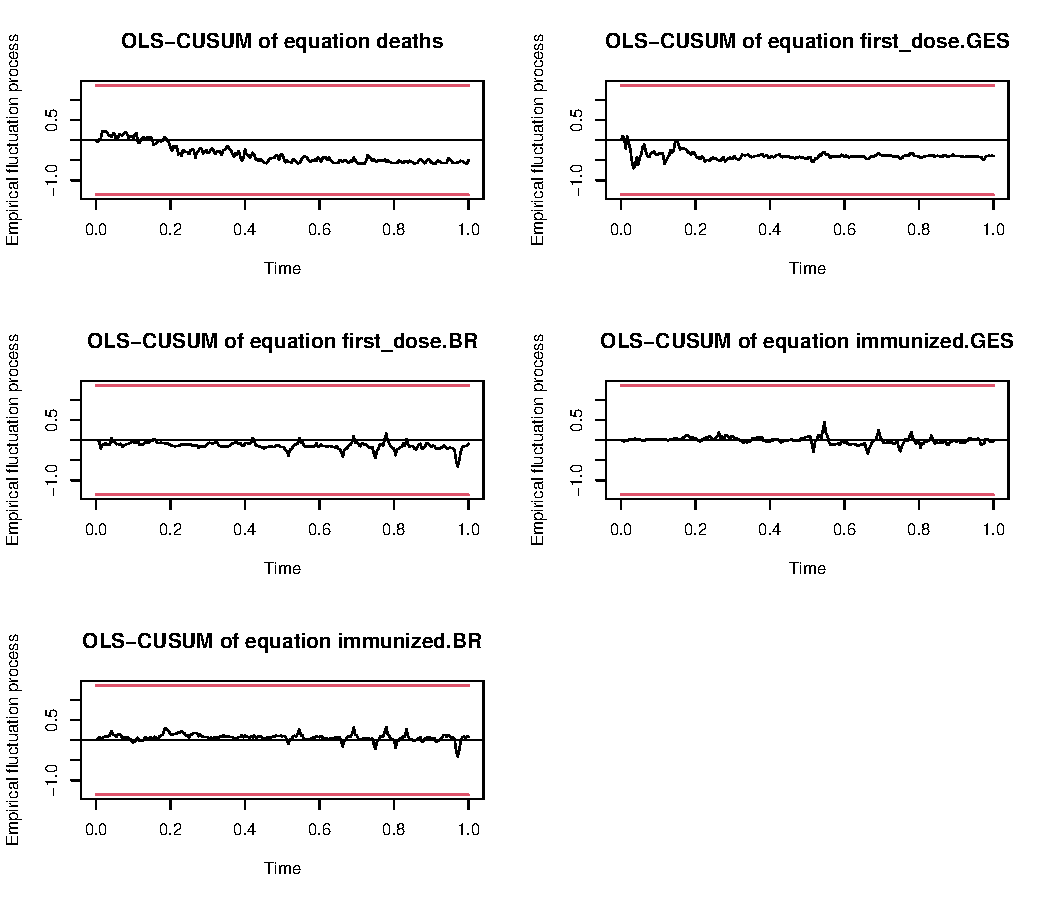
\includegraphics[width=\linewidth]{IF_results_ENG_files/figure-latex/unnamed-chunk-36-1} \end{center}

\textbf{Figure 25}: structural stability test of residuals with 95\%
confidence bands.

In Figure 24, we can see that there is no structural irregularity since
no residual curve exceeds the confidence bands.

Another point that we must check is the normality of the residuals.
Since we are in a multivariate problem, we want to test whether the
residuals follow a Gaussian or a multivariate normal distribution. When
we refer only as normal distribution, we imply that it is a univariate
distribution, which is not our case, so there is an importance in making
this distinction. Although it is an important step, it will not be a
requirement for the construction of impulse response functions, since
their confidence intervals will be built using bootstrap.

\begin{Shaded}
\begin{Highlighting}[]
\FunctionTok{normality.test}\NormalTok{(var1, }\AttributeTok{multivariate.only =} \ConstantTok{TRUE}\NormalTok{)}
\end{Highlighting}
\end{Shaded}

\begin{verbatim}
## $JB
## 
##  JB-Test (multivariate)
## 
## data:  Residuals of VAR object var1
## Chi-squared = 599.85, df = 10, p-value < 2.2e-16
## 
## 
## $Skewness
## 
##  Skewness only (multivariate)
## 
## data:  Residuals of VAR object var1
## Chi-squared = 16.175, df = 5, p-value = 0.006363
## 
## 
## $Kurtosis
## 
##  Kurtosis only (multivariate)
## 
## data:  Residuals of VAR object var1
## Chi-squared = 583.68, df = 5, p-value < 2.2e-16
\end{verbatim}

The normality test applied is called Jarque-Bera, which is a common test
to be applied in time series. The test points with a 5\% significance
level that the residuals do not follow a Gaussian distribution.

\subsection{Granger Causality}\label{granger-causality}

An interesting tool in time series is the Granger Causality Test.
Consider \(X\) and \(Y\) two time series, we say that \(X\) Granger
causes \(Y\) if the lagged values of \(X\) contribute significantly to
determining the present values of \(Y\), regardless of past values of
\(Y\) . In other words, past values of \(X\) are relevant to predicting
\(Y\). With this, we are able to get a sense of whether the past values
of the vaccination series had any influence on the values of the series
of deaths that we observed.

The Granger Causality Test will be applied in a multivariate way, so
that it will tell us if the series we are putting as a cause is Granger
causing the values of the other series in the model. The null hypothesis
of the test is that the series we are treating as the cause does not
Granger-cause the other series (within a single system, not
individually). In practice, If the null hypothesis is rejected, the test
does not say exactly whether the series we are putting as a cause,
Granger causes a specific series.

\begin{Shaded}
\begin{Highlighting}[]
\CommentTok{\# First dose BR as a cause}
\NormalTok{c1 }\OtherTok{\textless{}{-}} \FunctionTok{causality}\NormalTok{(var1, }\AttributeTok{cause =} \StringTok{"first\_dose.BR"}\NormalTok{)}
\NormalTok{c1}\SpecialCharTok{$}\NormalTok{Granger}
\end{Highlighting}
\end{Shaded}

\begin{verbatim}
## 
##  Granger causality H0: first_dose.BR do not Granger-cause deaths
##  immunized.BR first_dose.GES immunized.GES
## 
## data:  VAR object var1
## F-Test = 3.795, df1 = 8, df2 = 1150, p-value = 0.0002076
\end{verbatim}

\begin{Shaded}
\begin{Highlighting}[]
\CommentTok{\# Immunized BR as a cause}
\NormalTok{c2 }\OtherTok{\textless{}{-}} \FunctionTok{causality}\NormalTok{(var1, }\AttributeTok{cause =} \StringTok{"immunized.BR"}\NormalTok{)}
\NormalTok{c2}\SpecialCharTok{$}\NormalTok{Granger}
\end{Highlighting}
\end{Shaded}

\begin{verbatim}
## 
##  Granger causality H0: immunized.BR do not Granger-cause deaths
##  first_dose.BR first_dose.GES immunized.GES
## 
## data:  VAR object var1
## F-Test = 0.92248, df1 = 8, df2 = 1150, p-value = 0.4967
\end{verbatim}

\begin{Shaded}
\begin{Highlighting}[]
\CommentTok{\# First dose pregnant women as a cause}
\NormalTok{c3 }\OtherTok{\textless{}{-}} \FunctionTok{causality}\NormalTok{(var1, }\AttributeTok{cause =} \StringTok{"first\_dose.GES"}\NormalTok{)}
\NormalTok{c3}\SpecialCharTok{$}\NormalTok{Granger}
\end{Highlighting}
\end{Shaded}

\begin{verbatim}
## 
##  Granger causality H0: first_dose.GES do not Granger-cause deaths
##  first_dose.BR immunized.BR immunized.GES
## 
## data:  VAR object var1
## F-Test = 2.0541, df1 = 8, df2 = 1150, p-value = 0.03752
\end{verbatim}

\begin{Shaded}
\begin{Highlighting}[]
\CommentTok{\# Immunized pregnant women as a cause}
\NormalTok{c4 }\OtherTok{\textless{}{-}} \FunctionTok{causality}\NormalTok{(var1, }\AttributeTok{cause =} \StringTok{"immunized.GES"}\NormalTok{)}
\NormalTok{c4}\SpecialCharTok{$}\NormalTok{Granger}
\end{Highlighting}
\end{Shaded}

\begin{verbatim}
## 
##  Granger causality H0: immunized.GES do not Granger-cause deaths
##  first_dose.BR immunized.BR first_dose.GES
## 
## data:  VAR object var1
## F-Test = 2.1054, df1 = 8, df2 = 1150, p-value = 0.03266
\end{verbatim}

The Granger Causality Tests applied above indicate that among the 4
vaccination series we are studying, only the series of the immunized
Brazilian population does not Granger causes the observed values of the
other series, including the series of deaths. The test points out that
the other series of vaccinations have some causal Granger effect, but
does not specify in which series.

\subsection{Impulse response
functions(IRF)}\label{impulse-response-functionsirf}

In order to be able to assess more clearly the possible impact of
vaccination series on deaths, we will now build impulse response graphs.
We have 4 graphs where each one will have a series of vaccinations that
will serve as an impulse to carry out the structural shock, and in all
of them we will visualize the response in the deaths of pregnant and
postpartum women.

\begin{Shaded}
\begin{Highlighting}[]
\NormalTok{nahead }\OtherTok{\textless{}{-}} \DecValTok{14}
\NormalTok{runs }\OtherTok{\textless{}{-}} \DecValTok{100}
\NormalTok{orto\_irf }\OtherTok{\textless{}{-}} \ConstantTok{TRUE}
\CommentTok{\# impulse response functions}
\NormalTok{feir1 }\OtherTok{\textless{}{-}} \FunctionTok{irf}\NormalTok{(var1,}
             \AttributeTok{impulse =} \StringTok{"first\_dose.BR"}\NormalTok{,}
             \AttributeTok{response =} \FunctionTok{c}\NormalTok{(}\StringTok{"deaths"}\NormalTok{),}
             \AttributeTok{n.ahead =}\NormalTok{ nahead,}
             \AttributeTok{ortho =}\NormalTok{ orto\_irf,}
             \AttributeTok{runs =}\NormalTok{ runs,}
             \AttributeTok{cumulative =} \ConstantTok{TRUE}\NormalTok{,}
             \AttributeTok{boot =} \ConstantTok{TRUE}\NormalTok{, }
             \AttributeTok{ci =} \FloatTok{0.95}\NormalTok{)}

\NormalTok{feir2 }\OtherTok{\textless{}{-}} \FunctionTok{irf}\NormalTok{(var1,}
             \AttributeTok{impulse =} \StringTok{"immunized.BR"}\NormalTok{,}
             \AttributeTok{response =} \FunctionTok{c}\NormalTok{(}\StringTok{"deaths"}\NormalTok{),}
             \AttributeTok{n.ahead =}\NormalTok{ nahead,}
             \AttributeTok{ortho =}\NormalTok{ orto\_irf,}
             \AttributeTok{runs =}\NormalTok{ runs,}
             \AttributeTok{cumulative =} \ConstantTok{TRUE}\NormalTok{,}
             \AttributeTok{boot =} \ConstantTok{TRUE}\NormalTok{,}
             \AttributeTok{ic =} \FloatTok{0.95}\NormalTok{,}
             \AttributeTok{plot.type =} \StringTok{"multiple"}\NormalTok{)}

\NormalTok{feir3 }\OtherTok{\textless{}{-}} \FunctionTok{irf}\NormalTok{(var1,}
             \AttributeTok{impulse =} \StringTok{"first\_dose.GES"}\NormalTok{,}
             \AttributeTok{response =}\FunctionTok{c}\NormalTok{(}\StringTok{"deaths"}\NormalTok{),}
             \AttributeTok{n.ahead =}\NormalTok{ nahead,}
             \AttributeTok{ortho =}\NormalTok{ orto\_irf,}
             \AttributeTok{runs =}\NormalTok{ runs,}
             \AttributeTok{cumulative =} \ConstantTok{TRUE}\NormalTok{,}
             \AttributeTok{boot =} \ConstantTok{TRUE}\NormalTok{,}
             \AttributeTok{ic =} \FloatTok{0.95}\NormalTok{)}

\NormalTok{feir4 }\OtherTok{\textless{}{-}} \FunctionTok{irf}\NormalTok{(var1,}
             \AttributeTok{impulse =} \StringTok{"immunized.GES"}\NormalTok{,}
             \AttributeTok{response =} \FunctionTok{c}\NormalTok{(}\StringTok{"deaths"}\NormalTok{),}
             \AttributeTok{n.ahead =}\NormalTok{ nahead,}
             \AttributeTok{ortho =}\NormalTok{ orto\_irf,}
             \AttributeTok{runs =}\NormalTok{ runs,}
             \AttributeTok{cumulative =} \ConstantTok{TRUE}\NormalTok{,}
             \AttributeTok{boot =} \ConstantTok{TRUE}\NormalTok{,}
             \AttributeTok{ic =} \FloatTok{0.95}\NormalTok{)}

\CommentTok{\# extract\_varirf() extracts IRF estimates so we can use them freely}
\CommentTok{\# https://raw.githubusercontent.com/anguyen1210/var{-}tools/master/R/extract\_varirf.R}

\CommentTok{\# Orthogonal Impulse Response from partially vaccinated Brazil (cumulative)}
\NormalTok{feir1\_varirf }\OtherTok{\textless{}{-}} \FunctionTok{extract\_varirf}\NormalTok{(feir1)}
\NormalTok{plot1 }\OtherTok{\textless{}{-}}\NormalTok{ feir1\_varirf }\SpecialCharTok{\%\textgreater{}\%} 
  \FunctionTok{ggplot}\NormalTok{(}\FunctionTok{aes}\NormalTok{(}\AttributeTok{x =}\NormalTok{ period, }
             \AttributeTok{y =}\NormalTok{ irf\_first\_dose.br\_deaths, }
             \AttributeTok{ymin =}\NormalTok{ lower\_first\_dose.br\_deaths, }
             \AttributeTok{ymax =}\NormalTok{ upper\_first\_dose.br\_deaths)) }\SpecialCharTok{+}
  \FunctionTok{geom\_hline}\NormalTok{(}\AttributeTok{yintercept =} \DecValTok{0}\NormalTok{, }\AttributeTok{color =} \StringTok{"red"}\NormalTok{) }\SpecialCharTok{+}
  \FunctionTok{geom\_ribbon}\NormalTok{(}\AttributeTok{fill =} \ConstantTok{NA}\NormalTok{, }
              \AttributeTok{color =} \StringTok{"red"}\NormalTok{,}
              \AttributeTok{linetype =} \StringTok{"dashed"}\NormalTok{) }\SpecialCharTok{+}
  \FunctionTok{geom\_line}\NormalTok{() }\SpecialCharTok{+}
  \FunctionTok{theme\_bw}\NormalTok{() }\SpecialCharTok{+}
  \FunctionTok{ggtitle}\NormalTok{(}\StringTok{"Orthogonal IRF from partially vaccinated Brazil (cumulative)"}\NormalTok{)}\SpecialCharTok{+}
  \FunctionTok{ylab}\NormalTok{(}\StringTok{"Deaths"}\NormalTok{)}\SpecialCharTok{+}
  \FunctionTok{xlab}\NormalTok{(}\StringTok{"}\SpecialCharTok{\textbackslash{}n}\StringTok{95\% Bootstrap CI, 100 runs"}\NormalTok{) }\SpecialCharTok{+} 
  \FunctionTok{scale\_x\_continuous}\NormalTok{(}\AttributeTok{breaks =} \DecValTok{0}\SpecialCharTok{:}\NormalTok{nahead) }\SpecialCharTok{+}
  \FunctionTok{coord\_cartesian}\NormalTok{(}\AttributeTok{ylim =} \FunctionTok{c}\NormalTok{(}\SpecialCharTok{{-}} \FloatTok{0.07}\NormalTok{, }\FloatTok{0.06}\NormalTok{)) }\SpecialCharTok{+}
  \FunctionTok{theme}\NormalTok{(}\AttributeTok{panel.grid.minor =} \FunctionTok{element\_line}\NormalTok{(}\AttributeTok{color =} \StringTok{\textquotesingle{}white\textquotesingle{}}\NormalTok{),}
        \AttributeTok{panel.grid.major =} \FunctionTok{element\_line}\NormalTok{(}\AttributeTok{color =} \StringTok{\textquotesingle{}white\textquotesingle{}}\NormalTok{),}
        \AttributeTok{plot.title =} \FunctionTok{element\_text}\NormalTok{(}\AttributeTok{size =} \FloatTok{7.7}\NormalTok{),}
        \AttributeTok{axis.text =} \FunctionTok{element\_text}\NormalTok{(}\AttributeTok{size =} \DecValTok{7}\NormalTok{))}

\CommentTok{\# Orthogonal Impulse Response from Fully vaccinated Brazil (cumulative)}
\NormalTok{feir2\_varirf }\OtherTok{\textless{}{-}} \FunctionTok{extract\_varirf}\NormalTok{(feir2)}
\NormalTok{plot2 }\OtherTok{\textless{}{-}}\NormalTok{ feir2\_varirf }\SpecialCharTok{\%\textgreater{}\%} 
  \FunctionTok{ggplot}\NormalTok{(}\FunctionTok{aes}\NormalTok{(}\AttributeTok{x =}\NormalTok{ period, }
             \AttributeTok{y =}\NormalTok{ irf\_immunized.br\_deaths, }
             \AttributeTok{ymin =}\NormalTok{ lower\_immunized.br\_deaths, }
             \AttributeTok{ymax =}\NormalTok{ upper\_immunized.br\_deaths)) }\SpecialCharTok{+}
  \FunctionTok{geom\_hline}\NormalTok{(}\AttributeTok{yintercept =} \DecValTok{0}\NormalTok{, }\AttributeTok{color =} \StringTok{"red"}\NormalTok{) }\SpecialCharTok{+}
  \FunctionTok{geom\_ribbon}\NormalTok{(}\AttributeTok{fill =} \ConstantTok{NA}\NormalTok{, }
              \AttributeTok{color =} \StringTok{"red"}\NormalTok{,}
              \AttributeTok{linetype =} \StringTok{"dashed"}\NormalTok{) }\SpecialCharTok{+}
  \FunctionTok{geom\_line}\NormalTok{() }\SpecialCharTok{+}
  \FunctionTok{theme\_bw}\NormalTok{() }\SpecialCharTok{+}
  \FunctionTok{ggtitle}\NormalTok{(}\StringTok{"Orthogonal IRF from fully vaccinated Brazil (cumulative)"}\NormalTok{)}\SpecialCharTok{+}
  \FunctionTok{ylab}\NormalTok{(}\StringTok{"Deaths"}\NormalTok{)}\SpecialCharTok{+}
  \FunctionTok{xlab}\NormalTok{(}\StringTok{"}\SpecialCharTok{\textbackslash{}n}\StringTok{95\% Bootstrap CI, 100 runs"}\NormalTok{) }\SpecialCharTok{+} 
  \FunctionTok{scale\_x\_continuous}\NormalTok{(}\AttributeTok{breaks =} \DecValTok{0}\SpecialCharTok{:}\NormalTok{nahead) }\SpecialCharTok{+}
  \FunctionTok{coord\_cartesian}\NormalTok{(}\AttributeTok{ylim =} \FunctionTok{c}\NormalTok{(}\SpecialCharTok{{-}} \FloatTok{0.07}\NormalTok{, }\FloatTok{0.06}\NormalTok{)) }\SpecialCharTok{+}
  \FunctionTok{theme}\NormalTok{(}\AttributeTok{panel.grid.minor =} \FunctionTok{element\_line}\NormalTok{(}\AttributeTok{color =} \StringTok{\textquotesingle{}white\textquotesingle{}}\NormalTok{),}
        \AttributeTok{panel.grid.major =} \FunctionTok{element\_line}\NormalTok{(}\AttributeTok{color =} \StringTok{\textquotesingle{}white\textquotesingle{}}\NormalTok{),}
        \AttributeTok{plot.title =} \FunctionTok{element\_text}\NormalTok{(}\AttributeTok{size =} \FloatTok{7.7}\NormalTok{),}
        \AttributeTok{axis.text =} \FunctionTok{element\_text}\NormalTok{(}\AttributeTok{size =} \DecValTok{7}\NormalTok{))}

\CommentTok{\# Orthogonal Impulse Response from Partially vaccinated pregnant and postpartum (cumulative)}
\NormalTok{feir3\_varirf }\OtherTok{\textless{}{-}} \FunctionTok{extract\_varirf}\NormalTok{(feir3)}
\NormalTok{plot3 }\OtherTok{\textless{}{-}}\NormalTok{ feir3\_varirf }\SpecialCharTok{\%\textgreater{}\%} 
  \FunctionTok{ggplot}\NormalTok{(}\FunctionTok{aes}\NormalTok{(}\AttributeTok{x =}\NormalTok{ period, }
             \AttributeTok{y =}\NormalTok{ irf\_first\_dose.ges\_deaths, }
             \AttributeTok{ymin =}\NormalTok{ lower\_first\_dose.ges\_deaths, }
             \AttributeTok{ymax =}\NormalTok{ upper\_first\_dose.ges\_deaths)) }\SpecialCharTok{+}
  \FunctionTok{geom\_hline}\NormalTok{(}\AttributeTok{yintercept =} \DecValTok{0}\NormalTok{, }\AttributeTok{color =} \StringTok{"red"}\NormalTok{) }\SpecialCharTok{+}
  \FunctionTok{geom\_ribbon}\NormalTok{(}\AttributeTok{fill =} \ConstantTok{NA}\NormalTok{, }
              \AttributeTok{color =} \StringTok{"red"}\NormalTok{,}
              \AttributeTok{linetype =} \StringTok{"dashed"}\NormalTok{) }\SpecialCharTok{+}
  \FunctionTok{geom\_line}\NormalTok{() }\SpecialCharTok{+}
  \FunctionTok{theme\_bw}\NormalTok{() }\SpecialCharTok{+}
  \FunctionTok{ggtitle}\NormalTok{(}\StringTok{"Orthogonal IRF from partially vaccinated pregnant and postpartum (cumulative)"}\NormalTok{)}\SpecialCharTok{+}
  \FunctionTok{ylab}\NormalTok{(}\StringTok{"Deaths"}\NormalTok{)}\SpecialCharTok{+}
  \FunctionTok{xlab}\NormalTok{(}\StringTok{"}\SpecialCharTok{\textbackslash{}n}\StringTok{95\% Bootstrap CI, 100 runs"}\NormalTok{) }\SpecialCharTok{+} 
  \FunctionTok{scale\_x\_continuous}\NormalTok{(}\AttributeTok{breaks =} \DecValTok{0}\SpecialCharTok{:}\NormalTok{nahead) }\SpecialCharTok{+}
  \FunctionTok{coord\_cartesian}\NormalTok{(}\AttributeTok{ylim =} \FunctionTok{c}\NormalTok{(}\SpecialCharTok{{-}} \FloatTok{0.07}\NormalTok{, }\FloatTok{0.06}\NormalTok{)) }\SpecialCharTok{+}
  \FunctionTok{theme}\NormalTok{(}\AttributeTok{panel.grid.minor =} \FunctionTok{element\_line}\NormalTok{(}\AttributeTok{color =} \StringTok{\textquotesingle{}white\textquotesingle{}}\NormalTok{),}
        \AttributeTok{panel.grid.major =} \FunctionTok{element\_line}\NormalTok{(}\AttributeTok{color =} \StringTok{\textquotesingle{}white\textquotesingle{}}\NormalTok{),}
        \AttributeTok{plot.title =} \FunctionTok{element\_text}\NormalTok{(}\AttributeTok{size =} \FloatTok{7.7}\NormalTok{),}
        \AttributeTok{axis.text =} \FunctionTok{element\_text}\NormalTok{(}\AttributeTok{size =} \DecValTok{7}\NormalTok{))}

\CommentTok{\# Orthogonal Impulse Response from Fully vaccinated pregnant and postpartum (cumulative)}
\NormalTok{feir4\_varirf }\OtherTok{\textless{}{-}} \FunctionTok{extract\_varirf}\NormalTok{(feir4)}
\NormalTok{plot4 }\OtherTok{\textless{}{-}}\NormalTok{ feir4\_varirf }\SpecialCharTok{\%\textgreater{}\%} 
  \FunctionTok{ggplot}\NormalTok{(}\FunctionTok{aes}\NormalTok{(}\AttributeTok{x =}\NormalTok{ period, }
             \AttributeTok{y =}\NormalTok{ irf\_immunized.ges\_deaths, }
             \AttributeTok{ymin =}\NormalTok{ lower\_immunized.ges\_deaths, }
             \AttributeTok{ymax =}\NormalTok{ upper\_immunized.ges\_deaths)) }\SpecialCharTok{+}
  \FunctionTok{geom\_hline}\NormalTok{(}\AttributeTok{yintercept =} \DecValTok{0}\NormalTok{, }\AttributeTok{color =} \StringTok{"red"}\NormalTok{) }\SpecialCharTok{+}
  \FunctionTok{geom\_ribbon}\NormalTok{(}\AttributeTok{fill =} \ConstantTok{NA}\NormalTok{, }
              \AttributeTok{color =} \StringTok{"red"}\NormalTok{,}
              \AttributeTok{linetype =} \StringTok{"dashed"}\NormalTok{) }\SpecialCharTok{+}
  \FunctionTok{geom\_line}\NormalTok{() }\SpecialCharTok{+}
  \FunctionTok{theme\_bw}\NormalTok{() }\SpecialCharTok{+}
  \FunctionTok{ggtitle}\NormalTok{(}\StringTok{"Orthogonal IRF from fully vaccinated pregnant and postpartum (cumulative)"}\NormalTok{)}\SpecialCharTok{+}
  \FunctionTok{ylab}\NormalTok{(}\StringTok{"Deaths"}\NormalTok{)}\SpecialCharTok{+}
  \FunctionTok{xlab}\NormalTok{(}\StringTok{"}\SpecialCharTok{\textbackslash{}n}\StringTok{95\% Bootstrap CI, 100 runs"}\NormalTok{) }\SpecialCharTok{+} 
  \FunctionTok{scale\_x\_continuous}\NormalTok{(}\AttributeTok{breaks =} \DecValTok{0}\SpecialCharTok{:}\NormalTok{nahead) }\SpecialCharTok{+}
  \FunctionTok{coord\_cartesian}\NormalTok{(}\AttributeTok{ylim =} \FunctionTok{c}\NormalTok{(}\SpecialCharTok{{-}} \FloatTok{0.07}\NormalTok{, }\FloatTok{0.06}\NormalTok{)) }\SpecialCharTok{+}
  \FunctionTok{theme}\NormalTok{(}\AttributeTok{panel.grid.minor =} \FunctionTok{element\_line}\NormalTok{(}\AttributeTok{color =} \StringTok{\textquotesingle{}white\textquotesingle{}}\NormalTok{),}
        \AttributeTok{panel.grid.major =} \FunctionTok{element\_line}\NormalTok{(}\AttributeTok{color =} \StringTok{\textquotesingle{}white\textquotesingle{}}\NormalTok{),}
        \AttributeTok{plot.title =} \FunctionTok{element\_text}\NormalTok{(}\AttributeTok{size =} \FloatTok{7.7}\NormalTok{),}
        \AttributeTok{axis.text =} \FunctionTok{element\_text}\NormalTok{(}\AttributeTok{size =} \DecValTok{7}\NormalTok{))}

\NormalTok{(plot1 }\SpecialCharTok{|}\NormalTok{ plot2) }\SpecialCharTok{/}\NormalTok{ (plot3 }\SpecialCharTok{|}\NormalTok{ plot4)}
\end{Highlighting}
\end{Shaded}

\begin{center}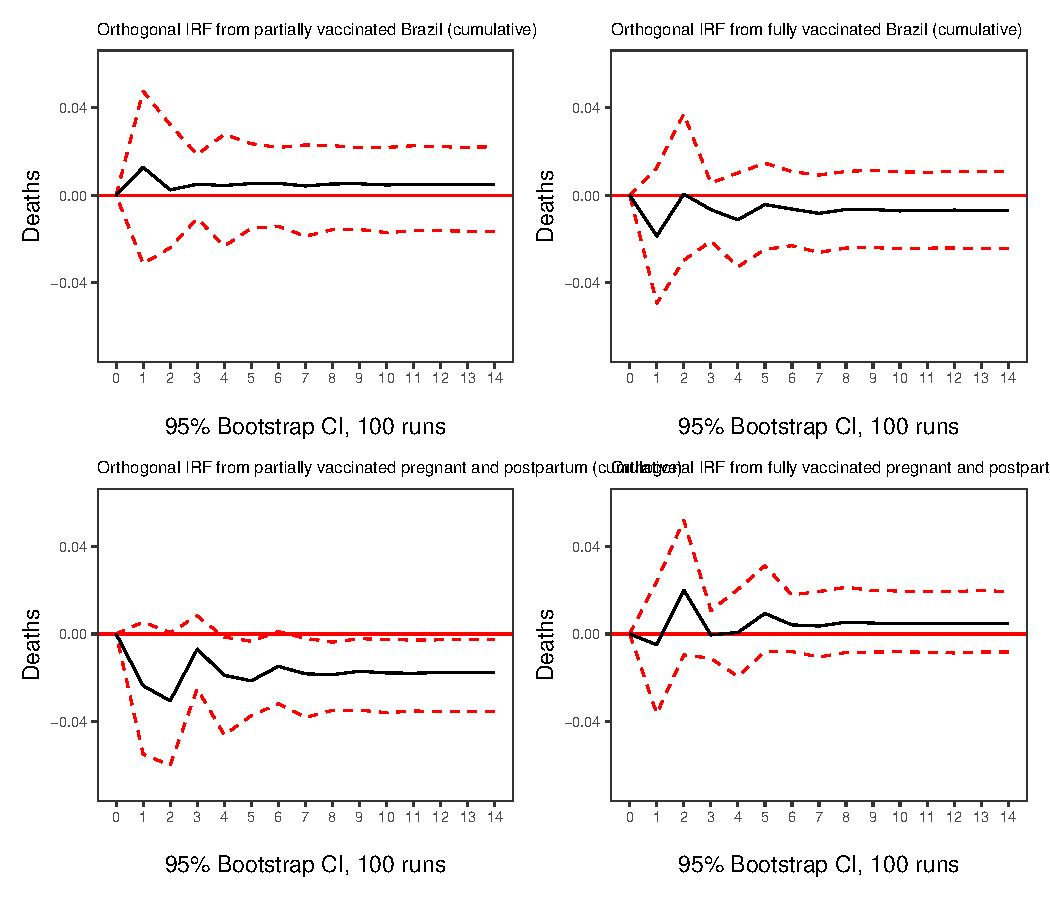
\includegraphics[width=\linewidth]{IF_results_ENG_files/figure-latex/unnamed-chunk-40-1} \end{center}

\textbf{Figure 26}: Orthogonal Impulse Response Functions (black line)
over 14 days for each vaccination series with 95\% confidence bands
(dashed red curves) calculated using bootstrap. The ``partially
vaccinated'' refer to the series of the first dose of the COVID-19
vaccine of their respective group (Brazil or pregnant and postpartum
women). The ``fully vaccinated'' refer to populations (Brazil or
pregnant and postpartum women) who took a second dose or booster, which
we have called immunized.

In Figure 25, we can visualize the impact of each vaccination series on
the deaths of pregnant and postpartum women. We can notice that, for all
the vaccination series we had an immediate impact on the series of
deaths, however, we see that the impact generated by the series of
vaccination with the first dose of the vaccine of the maternal
population (partially vaccinated pregnant and postpartum) was reasonably
greater than the others. Note that, after the initial ``jump'', the IRF
of the vaccination with the first dose series of the maternal population
remained the furthest away from zero over time. This shows that the
first dose of the vaccine against COVID-19 in pregnant and postpartum
women in Brazil, when compared to the vaccination of the general
population and the second dose or booster of the maternal population,
was the factor that, not only had the greatest immediate impact on the
fall of deaths in the month of May in 2021, as it was also the factor
that held back the downward behavior more intensely over time.

\end{document}
